\documentclass[12pt]{article}

%------------------------------------------%
%                Packages
%------------------------------------------%
%These are the packages that we will use in our latex document. 
\usepackage{clipboard}%For copy past text in different parts of document
\usepackage{amsmath, amssymb,mathrsfs} %For using math
\usepackage{color}
\usepackage{enumitem}
\usepackage{graphicx}
\usepackage{grffile}
\usepackage[utf8]{inputenx}% For proper input encoding
\usepackage{mathptmx}
\usepackage{pdflscape}
\usepackage{soul}
%\usepackage{libertine}% Linux Libertine, may favourite text font
\usepackage[euler-digits]{eulervm}% A pretty math font

%\usepackage{fontspec}
%\usepackage{unicode-math}

%\setmainfont{Linux Libertine O}

%\newcommand{\setlibertinemath}{%
% use Libertine for the letters
%\setmathfont[range=\mathit/{latin,Latin,num,Greek,greek}]{Linux Libertine O Italic}
%\setmathfont[range=\mathup/{latin,Latin,num,Greek,greek}]{Linux Libertine O}
%\setmathfont[range=\mathbfup/{latin,Latin,num,Greek,greek}]{Linux Libertine O Bold}
%\setmathfont[range={"2202}]{Linux Libertine O}% "02202 = \partial % doesn't work
%\setmathfont[range={"221E}]{Linux Libertine O}% "0221E = \infty
% etc. (list should be completed depending on needs)
%}



%%% ABSTRACT
\usepackage{abstract}
\renewcommand{\abstractname}{}    % clear the title
\renewcommand{\absnamepos}{empty} % originally center

%%% PAGE DIMENSIONS
\usepackage[margin=1in]{geometry} %For controlling the dimensions. Very useful for Posters, etc
% PAPER SIZE
\setlength\paperheight{11in}
\setlength\paperwidth{8.5in}
% MARGINS 
%\topmargin=-0.5in
\parskip=0pt
%\setlength\textwidth{135.5mm}
%\setlength\textheight{200mm}
%\setlength\topmargin{-10pt}
%\setlength\oddsidemargin{14mm}
%\setlength\evensidemargin{\oddsidemargin}
%\setlength\headheight{24pt}
%\setlength\headsep{14pt}
%\setlength\topskip{11.74pt}
%\setlength\maxdepth{.5\topskip}
%\setlength\footskip{15pt}

%%% HEADERS AND FOOTERS
\usepackage{fancyhdr}
%\pagestyle{plain} % options: empty , plain , fancy
%\renewcommand{\headrulewidth}{0pt} % customise the layout...
%\lhead{}\chead{}\rhead{}
%\lfoot{}\cfoot{\thepage}\rfoot{}

%%% SECTION TITLE APPEARANCE
%\usepackage{sectsty}
%%\sectionfont{\large}
%\sectionfont{\normalsize}
%\subsectionfont{\small}
%\paragraphfont{\small}
%\allsectionsfont{\mdseries\upshape 
%        \sectionrule{15pt}{0pt}{-5pt}{1pt} }
\usepackage{titlesec}
\titleformat*{\section}{\normalsize\bfseries}
\titleformat*{\subsection}{\small\bfseries}
\titleformat*{\subsubsection}{\small\bfseries}
\titleformat*{\paragraph}{\small\bfseries}
\titleformat*{\subparagraph}{\small\bfseries}
\titlespacing\section{0pt}{6pt plus 4pt minus 2pt}{0pt plus 2pt minus 2pt}
\titlespacing\subsection{0pt}{6pt plus 4pt minus 2pt}{0pt plus 2pt minus 2pt}
\titlespacing\subsubsection{0pt}{6pt plus 4pt minus 2pt}{0pt plus 2pt minus 2pt}
\titlespacing\paragraph{0pt}{6pt plus 4pt minus 2pt}{6pt plus 2pt minus 2pt}

%%% CITATIONS
\usepackage[authoryear]{natbib}	%Bibliography package. It handles citations and can easily change formats. This is done at the end of the document
\usepackage{multibib}
\newcites{App}{Appendix References}%  \citelatex, \nocitelatex, ...
\newcites{Ref}{References in Referee Replies}%  \citelatex, \nocitelatex, ...
\newcites{Main}{References}%  \citelatex, \nocitelatex, ...

\setcitestyle{aysep={}} 
%------------------------------------------%
%     Tables 
%------------------------------------------%
\usepackage{accents}
\usepackage{adjustbox} %Handles resizing of tables, figures, etc. Based off of page and/or line width/height 
\usepackage{bbm}
\usepackage{bm}
\usepackage{booktabs}% For Pretty tables
\usepackage{caption} %\captionsetup[figure]{justification=raggedright,singlelinecheck=off}
\captionsetup[table]{labelsep=period}
\captionsetup{labelsep=period}
\usepackage{chngpage} 
\usepackage{comment}
\usepackage{dcolumn}
%\usepackage{everypage}%For page numbers on rotated pages%Functionality added to latex
%\usepackage{float}
\usepackage[capposition=top]{floatrow}
\usepackage{morefloats}
\usepackage{multicol}
\usepackage{multirow}
\usepackage{placeins}% To Create Float Barriers so the tables will stay in their sections
\usepackage[list=true]{subcaption} %For having multiple figures within the same one. Figure 1, with part (a) and (b) %\setcounter{lofdepth}{2}
\usepackage{threeparttable}% For Notes below table
\usepackage{rotating}% To Rotate Table
\usepackage{setspace} %Single, Double Space, etc 
\usepackage{siunitx} %This aligns tables by their decimal and handles processing of the numbers within the tables
  \sisetup{
    detect-mode,
    group-digits      = false,
    input-symbols     = {( ) [ ] - +},
    table-align-text-post = false,
    input-signs             = ,
    %parse-numbers=false,
    %scientific-notation = true,
        %round-mode              = places,
        %round-precision         = 2,
    %input-ignore={,},
    input-decimal-markers={.},
    group-separator={,},
    %group-minimum-digits={4},
    %group-four-digits = true,
	separate-uncertainty=true,
	%zero-decimal-to-integer=true,
   } 
%------------------------------------------%
%     Formatting options 
%------------------------------------------%

\AtBeginDocument{
    \addtolength{\abovedisplayskip}{-1.0ex}
    \addtolength{\abovedisplayshortskip}{-1.0ex}
    \addtolength{\belowdisplayskip}{-1.0ex}
    \addtolength{\belowdisplayshortskip}{-1.0ex}
}
\setlength{\parskip}{\smallskipamount}%med
%\setlength{\parindent}{0pt}
\DeclareCaptionLabelFormat{blank}{}
\DeclareCaptionFormat{myformat}{
    \begin{varwidth}{\linewidth}
        \centering
        #1#2#3%
    \end{varwidth}
}
\usepackage{silence}
\WarningFilter*{latex}{Text page \thepage\space contains only floats}
\WarningFilter*{caption}{Ambiguous sub-caption}
\WarningFilter*{natbib}{Citation}
\WarningFilter{natbib}{Citation}

%------------------------------------------%
%     Hyper Ref 
%------------------------------------------%
%\usepackage{silence}
%\WarningFilter{hyperref}{You have enabled option `breaklinks'.}
\usepackage[unicode=true,pdfusetitle,bookmarks=true,bookmarksnumbered=false,bookmarksopen=false,breaklinks=true,pdfborder={0 0 1},backref=false,colorlinks=true,citecolor=black,allcolors=black,hyperfootnotes=true]{hyperref}
%\usepackage[unicode=true,pdfusetitle,bookmarks=true,bookmarksnumbered=false,bookmarksopen=false,breaklinks=true,pdfborder={0 0 1},backref=false,colorlinks=true,citecolor=black,hyperfootnotes=true]{hyperref}
\def\UrlBreaks{\do\/\do-\do.\do=\do_\do?\do\&\do\%\do\a\do\b\do\c\do\d\do\e\do\f\do\g\do\h\do\i\do\j\do\k\do\l\do\m\do\n\do\o\do\p\do\q\do\r\do\s\do\t\do\u\do\v\do\w\do\x\do\y\do\z\do\A\do\B\do\C\do\D\do\E\do\F\do\G\do\H\do\I\do\J\do\K\do\L\do\M\do\N\do\O\do\P\do\Q\do\R\do\S\do\T\do\U\do\V\do\W\do\X\do\Y\do\Z\do\0\do\1\do\2\do\3\do\4\do\5\do\6\do\7\do\8\do\9} 
%\usepackage[hyphenbreaks]{breakurl}
% hyperef does not work with beamer (as far as I know) so comment this out if you are using it. 
% Also leave the hyperfootnotes as false as when they are true they oddly clash with the caption or subcaption package.


%------------------------------------------%
%    Appendix
%------------------------------------------%
\usepackage[titletoc]{appendix}

%------------------------------------------%
%    To Do Notes
%------------------------------------------%

%\usepackage[colorinlistoftodos,prependcaption,textsize=tiny]{todonotes}
\usepackage{xcolor}
\usepackage{xargs}
%Use \todo to create a general todo item for anyone
%Something for Chris to do
%\newcommandx{\todochris}[2][1=]{\todo[linecolor=green,backgroundcolor=green!25,bordercolor=yellow,#1]{Chris: #2}}
%\newcommandx{\todokk}[2][1=]{\todo[linecolor=green,backgroundcolor=green!25,bordercolor=yellow,#1]{Chris: #2}}
%Something for Anthony to do
%\newcommandx{\todoanthony}[2][1=]{\todo[linecolor=green,backgroundcolor=green!25,bordercolor=yellow,#1]{Anthony: #2}}
% To just make a comment use this
%\newcommandx{\todocomment}[2][1=]{\todo[linecolor=yellow,backgroundcolor=yellow!25,bordercolor=cyan,#1]{Comment: #2}}
\renewcommand{\thefootnote}{\fnsymbol{footnote}}

\setlength{\marginparwidth}{2cm}
%\usepackage[colorinlistoftodos]{todonotes}
\usepackage{epigraph}
\setlength \epigraphwidth {\linewidth}
\setlength \epigraphrule {0pt}
\AtBeginDocument{\renewcommand {\epigraphflush}{center}}
\renewcommand {\sourceflush} {center}

%------------------------------------------%
%              Custom Commands
%------------------------------------------%
%These are the custom commands that I use in the latex document

\newcommand\iid{i.i.d.} %Makes iid a command
\newcommand\pN{\mathcal{N}} %Makes the natural numbers a command

\setcounter{MaxMatrixCols}{20}

\newtheorem{theorem}{Theorem}%[section]
\newtheorem{lemma}[theorem]{Lemma}
\newtheorem{proposition}[theorem]{Proposition}
\newtheorem{corollary}[theorem]{Corollary}
\newtheorem{assumption}[theorem]{Assumption}
\newenvironment{proof}{\paragraph{Proof:}}{\hfill$\square$ \\} %This fixes the problem with dynamic tables for some reason

%For Page Numbers while rotated
%\newlength{\hfoot}
%\newlength{\vfoot}
%\AddEverypageHook{\ifdim\textwidth=\linewidth\relax
%\else\setlength{\hfoot}{-\topmargin}%
%\addtolength{\hfoot}{-\headheight}%
%\addtolength{\hfoot}{-\headsep}%
%\addtolength{\hfoot}{-.5\linewidth}%
%\ifodd\value{page}\setlength{\vfoot}{\oddsidemargin}%
%\else\setlength{\vfoot}{\evensidemargin}\fi%
%\addtolength{\vfoot}{\textheight}%
%\addtolength{\vfoot}{\footskip}%
%\raisebox{\hfoot}[0pt][0pt]{\rlap{\hspace{\vfoot}\rotatebox[origin=cB]{90}{\thepage}}}\fi}
%http://tex.stackexchange.com/questions/209685/landscape-mode-and-page-numbering

%For figure notes
\newcommand{\Ftext}[1]{%
    \begin{minipage}[b]{1.0\linewidth}
        \vspace{2mm}
        \begin{flushleft}
            \subcaption*{#1}
        \end{flushleft}
    \end{minipage}
 }
\newcommand{\Fnote}[1]{\Ftext{\text{Notes:~}~#1}}
\newcommand{\FnoteScript}[1]{\Ftext{\text{\scriptsize{Notes:}~}~#1}}
\newcommand{\FnoteFoot}[1]{\Ftext{\text{\footnotesize{Notes:}~}~#1}}

%Math
\newcommand{\ev}[1]{\mathop{\mathbb E\,} \left[#1\right]}
\newcommand{\indep}{\perp \!\!\! \perp}
\newcommand{\var}{\operatorname{var}}
\newcommand{\cov}{\operatorname{cov}}

%------------------------------------------%
%      Matter Related to Table Creation
%------------------------------------------%
%This helps with custom automatic tables. It uses latex  functions
%http://www.jwe.cc/2012/03/stata-latex-tables-estout/
%http://repec.org/bocode/e/estout/estout.html

% *****************************************************************
% Estout related things
% *****************************************************************

% Added due to changes in TexLive 2022 breaking code
%https://www.overleaf.com/blog/tex-live-2022-now-available
%https://tex.stackexchange.com/questions/567985/problems-with-inputtable-tex-hline-after-2020-fall-latex-release
\makeatletter
%%primitive input in tabular
\AddToHook{env/tabular/begin}{\let\estinput=\@@input}
\makeatother
%\let\estinput=\@@input % define a new input command so that we can still flatten the document

\newcommand{\estwide}[3]{
    \vspace{.25ex}{
      \textsymbols% Note the added command here
      \begin{tabular*}
      {\textwidth}{@{\hskip\tabcolsep\extracolsep\fill}l*{#2}{#3}}
      \toprule
      \estinput #1 
      \bottomrule
      \addlinespace[.75ex]
      \end{tabular*}
      }
    } 

\newcommand{\estauto}[3]{
    \vspace{.25ex}{
      \textsymbols% Note the added command here
      \begin{tabular}{l*{#2}{#3}}
      \toprule
      \estinput #1 
      \bottomrule
      \addlinespace[.75ex]
      \end{tabular}
      }
    }

% Allow line breaks with \\ in specialcells
\newcommand{\specialcell}[2][c]{%
    \begin{tabular}[#1]{@{}c@{}}#2\end{tabular}
}
\DeclareUnicodeCharacter{00A0}{ }
% *****************************************************************
% Custom subcaptions
% *****************************************************************
% Note/Source/Text after Tables
% The new approach using threeparttables to generate notes that are the exact width of the table.
\newcommand{\Figtext}[1]{%
  \begin{tablenotes}[para,flushleft]
  %\hspace{6pt}
  %\hangindent=1.75em
  #1
  \end{tablenotes}
  }
\newcommand{\Fignote}[1]{\Figtext{\text{Notes:~}~#1}}
\newcommand{\Figsource}[1]{\Figtext{\text{Source:~}~#1}}
\newcommand{\Starnote}{\Figtext{Point estimates marked ***, **, and * are statistically significant at the 1, 5, and 10 percent levels, respectively.}}% Add significance note with \starnote
% If you are using hyper-ref (recommended), this command must go after all 
% other package inclusions (from the hyperref package documentation).
% The purpose of hyperref is to make the PDF created extensively
% cross-referenced.

\usepackage{ifthen}
\newboolean{stars_on}
\setboolean{stars_on}{false} % or {false}
\ifthenelse{\boolean{stars_on}}
{%
  % Text to include when stars_on is true
  \newcommand{\sym}[1]{\rlap{#1}}
  \newcommand{\nlsym}[1]{\rlap{\append{}{*}{#1}}}
  \newcommand{\pvaluenote}{* p $<$ 0.1, ** p $<$ 0.05, *** p $<$ 0.01. }
}
{%
  % Text to include when stars_on is false
  \newcommand{\sym}[1]{\rlap{~}}
  \newcommand{\nlsym}[1]{\rlap{\append{}{~}{#1}}}
  \newcommand{\pvaluenote}{}

}
 %Allows for fancy stars in tables that also works in beamer
% %Allows for fancy stars in tables that also works in beamer

% Create a function that works for the non-linear symbols
%\newcommand{\nlsym}[1]{\rlap{\append{}{*}{#1}}} %Allows for fancy stars in tables that also works in beamer
 %Allows for fancy stars in tables that also works in beamer

% Character substitution that prints brackets and the minus symbol in text mode. Thanks to David Carlisle
\def\yyy{%
  \bgroup\uccode`\~\expandafter`\string-%
  \uppercase{\egroup\edef~{\noexpand\text{\llap{\textendash}\relax}}}%
  \mathcode\expandafter`\string-"8000 }

\def\xxxl#1{%
\bgroup\uccode`\~\expandafter`\string#1%
\uppercase{\egroup\edef~{\noexpand\text{\noexpand\llap{\string#1}}}}%
\mathcode\expandafter`\string#1"8000 }

\def\xxxr#1{%
\bgroup\uccode`\~\expandafter`\string#1%
\uppercase{\egroup\edef~{\noexpand\text{\noexpand\rlap{\string#1}}}}%
\mathcode\expandafter`\string#1"8000 }

\def\textsymbols{\xxxl[\xxxr]\xxxl(\xxxr)\yyy}


%Protects against odd minus sign errors within the tables
\catcode`_11
\protected\def \c__siunitx_minus_tl {$-$}
\catcode`_ 8 

%-----------Tables-------------%
% This Section is needed to make the tables work with amsmath. But because of the \( being open and having no match, Sublime Text thinks that everything after it (all text) is in math mode and hence changes the text color. This annoys me so the only ``solution'' is to just place this preamble here. It seems to work still. 
\makeatletter 
\edef\originalbmathcode{%
    \noexpand\mathchardef\noexpand\@tempa\the\mathcode`\(\relax} %\)

\def\resetMathstrut@{%
  \setbox\z@\hbox{%
    \originalbmathcode

    \def\@tempb##1"##2##3{\the\textfont"##3\char"}%
    \expandafter\@tempb\meaning\@tempa \relax
  }%
  \ht\Mathstrutbox@\ht\z@ \dp\Mathstrutbox@\dp\z@
}
\makeatother %./tables.tex:25: LaTeX Error: Bad math environment delimiter. [\)]
\usepackage{xparse}

\ExplSyntaxOn
\DeclareExpandableDocumentCommand{\append}{mmm}
 {
  #1\prg_replicate:nn{#3}{#2}
 }
\ExplSyntaxOff

\doublespacing

%------------------------------------------%
% Check if figures are all mentioned in text
%------------------------------------------%
%\usepackage{refcheck}

\begin{document}
%------------------------------------------%
%     Title Page
%------------------------------------------%
    \newgeometry{top = 1in, bottom = 0.75in, right = 1in, left = 1in, footskip = 0.0in}
\begin{titlepage}
    \begin{center}
        \renewcommand{\thefootnote}{\fnsymbol{footnote}}
        \textbf{
        \noindent\LARGE
        \title
         ~The Gift of a Lifetime: The Hospital, Modern Medicine, and Mortality \footnote{{We thank Brian Beach, Brandyn Churchill, Jane Greve, Maggie Jones, Carl Kitchens, Peter Nencka, Greg Niemesh, and seminar/conference participants at the Atlanta-Athens Health Economists Research Conference, the Danish Society for Economic and Society History and Scandinavian Society of Economic and Social History annual meeting, the Essen Health Conference, the National Bureau of Economic Research (NBER) Health Economics Fall Meeting, the NBER Summer Institute Development of American Economy and Children's sessions, Duke University, Emory University, Indiana University, The Insper Institute of Education and Research, Lund University, Miami University, The Ohio State University Departments of Economics and Human Sciences, and the University of Copenhagen for helpful comments and feedback. We are grateful to Patrick Carlin and Mallory Dreyer for research assistance and Hardish Bindra at Paradigm Data Services. We would like to especially thank John Parman for sharing the North Carolina death certificate data. Thomasson acknowledges support from the Julian Lange Professorship. Wray appreciates financial support from the Japan Society for the Promotion of Science (KAKENHI Young Scientists B Grant Number J160100115), research funds from the Hitotsubashi Institute for Advanced Study (HIAS) at Hitotsubashi University, and an Arthur Cole Grant from the Economic History Association.}}
        }

        \vspace{.25cm}
        %\vspace{.4cm}
        {\large{\begin{tabular}{c c c}
{Alex Hollingsworth} &&  {Krzysztof Karbownik}  \vspace{-.4cm}\\
The Ohio State University and NBER && Emory University and NBER \\

{Melissa A. Thomasson} && {Anthony Wray}  \vspace{-.4cm} \\
Miami University and NBER && University of Southern Denmark   \\
\end{tabular}}}\\
        \vspace{.25cm}
        {\large\today}\

       \vspace{-.25cm}


    \end{center}

    \begin{abstract}
    \begin{normalsize}
    \begin{singlespace}
    \noindent
   % 100 words
    We explore how access to modern hospitals and medicine affects mortality by leveraging efforts of The Duke Endowment to modernize hospitals in the early-twentieth century. 
    The Endowment helped communities build and expand hospitals, obtain state-of-the-art medical technology, attract qualified medical personnel, and refine management practices. 
    We find that Duke support increased the size and quality of the medical sector, fostering growth in not-for-profit hospitals and high-quality physicians. 
    Duke funding reduced both infant mortality -- with larger effects for Black infants than White infants -- and long-run mortality. 
    Finally, we find that communities aided by Duke benefited more from medical innovations.

    \end{singlespace}
    \end{normalsize}
    \end{abstract}
               \vspace{-.5cm}

    \noindent\textbf{JEL Codes:} I14, J13, N32
    %\vspace{.4cm}
    \begin{singlespace}
    \noindent\textbf{Keywords:} modern medicine, hospitals, mortality, infant health, hospital funding, physician labor supply, medical innovation, health care complementarities, charitable giving
    \end{singlespace}
    \setcounter{footnote}{0}


\end{titlepage}
\restoregeometry
\newpage

%------------------------------------------%
%                Main text
%------------------------------------------%
 \FloatBarrier
 \renewcommand{\thefootnote}{\arabic{footnote}}

\setlength{\floatsep}{10pt}
\setlength{\textfloatsep}{0pt}
 %------------------------------------------%
%      Introduction
%------------------------------------------%

\onehalfspacing
%\section{Introduction} \label{sec:intro}

%%%%%%%%%%%%%%%%%%%%%%%%%%%%%%%%%%%%%%%%%%%%%%%%%%%%%%%%%%%%%%%%%%%%%%%
%                            Hook.                                    %
%%%%%%%%%%%%%%%%%%%%%%%%%%%%%%%%%%%%%%%%%%%%%%%%%%%%%%%%%%%%%%%%%%%%%%%

As medicine has advanced over the last century, spending on healthcare has risen to consume an ever-increasing share of resources. 
In 1900, healthcare represented only 2\% of US gross domestic product \citepMain{Craig2006}. 
By 2020, this share soared to 20\%, with spending on hospital care alone accounting for 6\% of US economic activity \citepMain{cms_nhe_2022}. 
This past century has also marked the rise of modern medicine and hospitals, transforming the institution ``from places of dreaded impurity and exiled human wreckage into awesome citadels of science and bureaucratic order'' \citepMain{starrSocialTransformationAmerican2017}. 
Building on gains over the mid- to late-nineteenth century -- attributable to rising incomes and better nutrition -- health has improved dramatically over the twentieth century, with infant mortality rates falling by 95\% and life expectancy at birth rising by 45\% \citepMain{costa2015Health1750On}. 
A large body of work has explored the drivers and the timing of this health transition. 
One claim from this literature is that modern medicine -- with the exception of sulfa drugs -- did not begin to materially affect health and mortality until after the 1950s \citepMain{cutlerYourMoneyYour2005}.
Despite this viewpoint, little is known about the origins of the modern hospital or the contribution of medical care in improving health in the first half of the twentieth century.



%%%%%%%%%%%%%%%%%%%%%%%%%%%%%%%%%%%%%%%%%%%%%%%%%%%%%%%%%%%%%%%%%%%%%%%
%                            Question.                                %
%%%%%%%%%%%%%%%%%%%%%%%%%%%%%%%%%%%%%%%%%%%%%%%%%%%%%%%%%%%%%%%%%%%%%%%

We seek to understand the role of funding for formal health care in improving health outcomes.
Did financial resources help to expand hospitals and attract higher-quality physicians with modern medical training? 
Did these improvements to medical care contribute to declining mortality during infancy and in the long run?
Given the many racial inequities in society and in health, were these effects similar or different by race?
And finally, did the modernization of hospitals allow for more productive use of new medical technologies?

%%%%%%%%%%%%%%%%%%%%%%%%%%%%%%%%%%%%%%%%%%%%%%%%%%%%%%%%%%%%%%%%%%%%%%%
%                  Empirical Approach.                                %
%%%%%%%%%%%%%%%%%%%%%%%%%%%%%%%%%%%%%%%%%%%%%%%%%%%%%%%%%%%%%%%%%%%%%%%

We leverage a combination of novel data and a unique quasi-experiment: a large-scale hospital modernization program introduced by The Duke Endowment in North Carolina during the first half of the twentieth century.
Beginning in 1927, The Duke Endowment funded capital projects to upgrade hospitals, thereby expanding access to modern medicine and hospital care across the Carolinas. 
It did so by placing a particular emphasis on rural and Black residents -- an uncommon approach in the Jim Crow-Era South.
The Endowment assisted hospitals in expanding and improving existing facilities, obtaining state-of-the art medical technology, and elevating their management practices.
In some communities, the Endowment helped to build new hospitals or to convert existing facilities to non-profits.
These modernization efforts were explicitly designed to attract higher-quality physicians to the Carolinas  \citepMain{duke1934,durdin1998}. 
By the end of 1942, the Endowment had appropriated over \$3.3 million (\$53 million in 2017 dollars) for hospital expansion and modernization in North Carolina, an investment that significantly improved access to medical facilities and the quality of the medical infrastructure, thereby propelling the practice of medicine in supported communities towards the modern era.\footnote{While The Duke Endowment operates in both North and South Carolina, we focus our analysis on North Carolina due to data availability as we discuss in Section ~\ref{sec:data}.}

Our main empirical approach is a difference-in-differences design that exploits quasi-random variation in Duke support, comparing counties that received a funding commitment from the Endowment to counties without such a commitment, and cohorts born before the initial commitment to those born after the introduction of Duke support.
In this effort, we construct a novel data set that combines information from hand-collected archival records, annual reports of The Duke Endowment, individual death certificates, physician directories, and a variety of other sources.
We opt for an extensive margin, intent-to-treat specification as our preferred model because treatment was not solely monetary.
To convert an appropriation into a payment, the Endowment typically required hospitals to undertake additional steps, such as changing accounting and record keeping practices; ensuring that surgeries were conducted by licensed physicians; allowing de facto inspections by Endowment employees; or forging community partnerships.
An intent-to-treat analysis captures the full effect of this multifaceted treatment, allowing for Duke support to both impact health before a single dollar was received and facilitate changes that improved health even in hospitals that never received a payment.

%%%%%%%%%%%%%%%%%%%%%%%%%%%%%%%%%%%%%%%%%%%%%%%%%%%%%%%%%%%%%%%%%%%%%%%
%                         Findings.                                %
%%%%%%%%%%%%%%%%%%%%%%%%%%%%%%%%%%%%%%%%%%%%%%%%%%%%%%%%%%%%%%%%%%%%%%%

We find that the efforts by Duke to modernize hospitals between 1927 and 1942 caused increases in hospital capacity and the quality of physicians. 
Duke support increased the number of hospital beds per 1,000 births in not-for-profit hospitals that were eligible for funding by 70.1\%, while causing a decline in ineligible for-profit beds of 61.4\%. 
Moreover, supported communities saw an increase in the number of high-quality physicians per 1,000 births of 60.2\% and a decrease in the number of poorly-trained physicians of 5.5\%, thereby advancing the average state of medical knowledge in locations supported by Duke. 

These first-stage effects and mechanisms help explain our core result that Duke financial support for the modernization of hospitals improved health, causing a 7.5\% reduction in the infant mortality rate. 
Treatment effect estimates for Black infants (13.6\%) are about three times as large as those for White infants (4.7\%). 
Those exposed to Duke support around the time of birth also enjoyed lasting health effects, as their long-run mortality rates (between the ages 56 and 64) declined by 9.0\%. 
Finally, we document that Duke-supported hospitals were able to use new medicines more effectively, suggesting a complementarity between high-quality hospitals and new medical innovations.

%%%%%%%%%%%%%%%%%%%%%%%%%%%%%%%%%%%%%%%%%%%%%%%%%%%%%%%%%%%%%%%%%%%%%%%
%                        Robustness.                                %   
%%%%%%%%%%%%%%%%%%%%%%%%%%%%%%%%%%%%%%%%%%%%%%%%%%%%%%%%%%%%%%%%%%%%%%%

Our findings are robust.
Point estimates and statistical significance are not materially affected by the choice of estimator, specification, transformation of the dependent variable, or sample decisions.
Our findings are also insensitive to the use of recent techniques that are robust to treatment effect heterogeneity and staggered treatment adoption in a difference-in-differences setting.
We further demonstrate that our results are not driven by the two primary threats to identification, differential pre-trends and selection into treatment. 
Across a number of event study specifications, outcomes in treated and control counties follow parallel trends prior to treatment. 
Using mortality data from other Southern states, we further confirm that the results are not driven by selection into treatment, by spillovers, or by the reallocation of medical expertise and investments within the Carolinas. 

%%%%%%%%%%%%%%%%%%%%%%%%%%%%%%%%%%%%%%%%%%%%%%%%%%%%%%%%%%%%%%%%%%%%%%%
%                  Cost-benefit analysis.                           %
%%%%%%%%%%%%%%%%%%%%%%%%%%%%%%%%%%%%%%%%%%%%%%%%%%%%%%%%%%%%%%%%%%%%%%%

The program was cost effective.
Considering only infant mortality from 1927 to 1942, one life was saved for every \$17,092 (2017 dollars) paid to hospitals, a cost significantly lower than any reasonable estimate for a Value of Statistical Life (VSL). 
The intervention was also particularly effective in reducing Black infant mortality, resulting in a mortality rate decrease much larger than the estimated decrease for White infants (a reduction of 15.1 vs.\ 3.1 deaths per 1,000 births) and narrowing the Black-White infant mortality gap by one-quarter. 
This new evidence that access to high-quality medical care and infrastructure disproportionately reduced Black mortality rates adds to previous work on the Black-White infant mortality gap, some of which finds that it has no relationship with increased healthcare access  \citepMain{collinsDecliningContributionSocioeconomic2004, elderRacialEthnicInfant2016,ACR2021,andersonWaterPurificationEfforts2021}.\footnote{The Duke Endowment's Indenture of Trust, written in the 1920s, explicitly stated that hospital access should be provided for \emph{both} Black and White individuals. Although Duke-supported hospitals remained segregated and care may not have been equal across race within the same hospital, the Endowment extended hospital access to Black residents in ways that were far from cosmetic. Before the Endowment's bi-racial mandate, many Black residents had no access to  hospital care, while afterwards ``all or practically all of the 65 hospital construction projects that the Endowment assisted during its first decade contained accommodations for both races'' \citepMain{durdin1998}.} 

%%%%%%%%%%%%%%%%%%%%%%%%%%%%%%%%%%%%%%%%%%%%%%%%%%%%%%%%%%%%%%%%%%%%%%%
%                         Value added (contribution).               %
%%%%%%%%%%%%%%%%%%%%%%%%%%%%%%%%%%%%%%%%%%%%%%%%%%%%%%%%%%%%%%%%%%%%%%%

This paper makes contributions to several literatures.
First, our findings contribute to a series of articles investigating the drivers of the health improvements observed in the early- to mid-twentieth century.
Most prior work focuses on the role of public health efforts \citepMain[e.g.,][]{ACR2022} or the advent of sulfa drugs \citepMain[e.g.,][]{TT2008, Jayachandran2010}.
Studies that examine the effects of hospitals or medical care on mortality have primarily concentrated on later time periods \citepMain{cutlerYourMoneyYour2005}.
For example, \citetMain{figinskiHealthInsuranceHospital2020} show that a rural hospital construction program in Appalachia in the 1950s improved infant health. 
Our results indicate that even earlier improvements in hospital construction and modernization reduced mortality, likely by attracting better-educated physicians to the area. 
Thus our findings suggest that improvements in medical care may have played a greater role in reducing mortality in the first half of the twentieth century than has been acknowledged.

Second, we build on the broader literature examining the short- and long-run consequences of prenatal and infant health. 
We also complement studies examining the determinants of mortal- ity and longevity, in which a common theme is that early life circumstances matter for later-life health \citepMain{almondChildhoodCircumstancesAdult2018}. 
Despite this large literature, ours is the first study to leverage quasi-experimental variation to show both the short- and long-run mortality consequences of a large hospital-funding program, and to our knowledge it is the first to examine whether hospital improvements in this time period helped to ameliorate long-standing racial gaps in mortality. 
A unique feature of our work is that we do not solely focus on applying a well-established intervention to a different vulnerable population. Instead, we analyze a bold experiment aimed at modernizing medical care during a critical phase in its development. 

Third, we contribute to the health care literature by demonstrating that high-quality facilities can have complementary effects.  We show that improving facilities attracted physicians who graduated from better medical schools. 
Such an outcome was a clear goal of The Duke Endowment, as the first director of the Endowment's Hospital Section, Dr.\ Watson S. Rankin, stated that  ``[t]he modern hospital$\ldots$ had come to play an essential part not only in the practice of medicine but also in the distribution of medical personnel'' and that creating well-supported hospitals would be ``the main remedy for the shortage of doctors'' \citepMain{durdin1998}. 
Our findings support this view. 

An additional complementarity that we examine is the relationship between technological innovation and improvements in physical and human capital, as discussed in \citetMain{AG2019}.
Specifically, we analyze the effect of the introduction of sulfa drugs in 1937, which resulted in significant reductions in infectious disease mortality \citepMain{TT2008,Jayachandran2010, Lazuka2020}. 
We demonstrate that Duke's emphasis on improving healthcare infrastructure and the quality of the medical workforce enabled communities to better leverage sulfa drugs, highlighting that the diffusion of knowledge is necessary for the effective spread and use of medical technologies \citepMain{soaresDeterminantsMortalityReductions2007}. 
Our findings reveal that in communities with higher baseline infectious disease mortality rates, the impact of The Duke Endowment's support on infant mortality approximately \emph{tripled} following the advent of sulfa drugs.

Fourth, we contribute to literature on management style, standardization, and firm performance \citepMain{bloomMeasuringExplainingManagement2007}. 
A distinct aspect of Duke support is that it was a multifaceted bundle of treatments coupled with ample oversight that was not limited to a monetary component. 
In addition to providing funding for facilities and equipment, the Endowment altered core management practices and standardized hospital accounting procedures.\footnote{Summarizing a letter written by Graham Davis, one-time assistant director of the Endowment, \citetMain{durdin1998} notes that ``the money they received from the Endowment was probably not as valuable to [the assisted hospitals] as the free service they got from the staff'' in the form of consulting, oversight, management expertise, and assistance in converting to uniform record keeping, of whom Duke-supported facilities ``were the largest group in the nation employing.''}
It thereby ``exerted considerable influence over the direction of hospital care'' in supported communities \citepMain{gambleMakingPlaceOurselves1995}.
Thus, it is unlikely that monetary assistance alone would have had the same effect. It is possible that the Duke intervention was so successful \emph{because} these many changes served to reinforce one another.

Finally, our work connects with the literature examining the effects of charitable contributions on public health and welfare, including the hookworm eradication campaign sponsored by the Rockefeller Sanitary Commission \citepMain{Bleakley2007}, and the Rosenwald Rural Schools Initiative \citepMain{AM2011, ALM2014}.  
For many years, The Duke Endowment was the third largest charity in the US and it remains one of the largest charitable foundations in the world \citepMain{durdin1998}. 
Despite its size and success, to our knowledge, virtually no others (outside of historians documenting Endowment activities) have attempted to evaluate the effects of the many programs that it operated. 

%%%%%%%%%%%%%%%%%%%%%%%%%%%%%%%%%%%%%%%%%%%%%%%%%%%%%%%%%%%%%%%%%%%%%%%
%                       Modern policy implications                  %
%%%%%%%%%%%%%%%%%%%%%%%%%%%%%%%%%%%%%%%%%%%%%%%%%%%%%%%%%%%%%%%%%%%%%%%

We view our results as having three important modern policy implications.
First, the success of the Endowment’s efforts to support hospitals was so pronounced that it  ``served as both inspiration and model'' for the Hill-Burton Act of 1946 \citepMain{durdin1998}, a large program designed to stimulate hospital construction and access across the US \citepMain{Chungetal}. 
Second, its impact in providing access to the first high-quality medical care facility in a community highlights the importance of attracting physicians to practice in under-served communities and the potential costs of closing rural hospitals today, as removing the last high-quality healthcare option may have a symmetric negative impact \citepMain{Kozhimannil2018, Germack2019, Fischer2022}.  
Third, our findings are relevant to healthcare investments in developing countries where donations from both private foundations and governments represent a major source of health financing \citepMain{Yamey2019}. 


%%%%%%%%%%%%%%%%%%%%%%%%%%%%%%%%%%
%%%%% Historical Background %%%%%%
%%%%%%%%%%%%%%%%%%%%%%%%%%%%%%%%%%

\section{The Duke Endowment and Hospital Care in North Carolina} \label{sec:Duke}

On December 11, 1924, James Buchanan Duke established The Duke Endowment with initial funding of \$40 million (\$563 million in 2017 dollars) to improve the social and economic welfare of communities in North and South Carolina.
In the Indenture of Trust for the Endowment, Duke acknowledged the vital role of hospitals as ``indispensable institutions'' for ``prolonging human life,'' noting that ``[t]he advance in the science of medicine'' has made ``hospital facilities essential for obtaining the best results in the practice of medicine'' \citepMain{Duke1925}.
Duke directed that 25.6\% of the income from the invested Endowment funds to be apportioned to the modernization, maintenance, and construction of not-for-profit hospitals \citepMain[p. 10-11]{Duke1925}.
Duke died unexpectedly in October 1925. His will left the Endowment with an additional \$69 million (\$972 million in 2017 dollars), with 90\% of the annual income from this contribution specifically directed to hospitals in the Carolinas \citepMain[p. 26]{durdin1998}.\footnote{Separately in his will, Duke earmarked \$4 million (\$56 million in 2017 dollars) to ``build and equip a medical school, hospital, and nurses' home at Duke University'' \citepMain[p. 26]{durdin1998}.} 

Another one of Duke's stated objectives in improving hospital facilities was to attract more highly-qualified doctors. In its inaugural report, the Hospital Section noted, ``Hospitals hold and attract the better type of physicians$\ldots$ So it is that a local hospital builds up a profession, raises professional standards and serves to improve the practice of medicine not only for patients in the hospital but for patients in the whole county'' \citepMain[144-45]{Duke1925}. This objective was realized in North Carolina, where physician density increased between 1923 and 1940 from 26 to 56 per 1,000 population.
The share of births in hospitals likewise increased, rising between 1931 and 1942 from 8.9\% to 34.2\%, but remained low even compared to the average of Southern states (13.2 \% in 1931 and 42\% in 1942).

Following Duke's death and prior to disbursement of any funds from the Endowment, the foundation surveyed the healthcare landscape in the Carolinas with a focus on the quality, size, and density of hospitals, as well as the supply of physicians.
Armed with this knowledge, the foundation started appropriating funds in 1927 -- the first year we consider a county to have been treated.
Panel A of Figure~\ref{fig:compare-roll-out-imr-changes} presents the share of North Carolina counties that received Duke appropriations by a specific year.
No appropriations were made prior to 1927; however, by 1929, almost 30\% of counties had been promised financial support.
In subsequent years, the geographic spread slowed, with the share increasing by only an additional 20 percentage points between 1929 and 1942. 
At the time, the modal treated county-year had only one hospital. 
We present the spatial distribution of first appropriations by county and year in panel B of Figure~\ref{fig:compare-roll-out-imr-changes}.

Although Black residents composed 30\% of the population in the Carolinas in 1924, they had far more limited access to hospitals than White residents due to institutionalized racial segregation.
The Duke Endowment paid ``special attention'' to racial equality when making funding decisions, and may have helped to narrow long-standing racial disparities in access to health care. In the period we study, The Endowment directed the vast majority of its support in North Carolina-- 75.5\% of appropriations and 74.0\% of payments-- to hospitals that accepted patients of both races. White-only hospitals received 15.6\% of capital appropriations (16.7\% of payments), while Black-only hospitals received 8.9\% (9.3\% of payments).\footnote{While the Endowment paid ``special attention [to] the needs of blacks in white-run biracial and black-run hospitals'' \citepMain{thomasDeluxeJimCrow2011}, \citetMain{gambleBlackAutonomyWhite1997} notes that this ``support, came at a price... The assisted facilities would be `for blacks' but would be supervised by whites.''
\citetMain{gambleMakingPlaceOurselves1995} cites specific examples, including changes at Lincoln Hospital where The Duke Endowment ``limited the access of black physicians to the operating room and insisted that all their work be supervised by white surgeons'' and replaced the Black superintendent with a White manager against the will of the surrounding Black community.
\citetMain{gambleMakingPlaceOurselves1995} argues that this ``arrangement frequently denied black people a voice in determining the direction of institutions which served them'' and  ``reinforced a racial hierarchy within medicine.'' She concludes that The Duke Endowment ``contributed to the advancement and maintenance of a separate, and not equal, medical world for black physicians, nurses and patients.''}



%------------------------------------------%
%      Data
%------------------------------------------%
\section{Data} \label{sec:data}


\subsection{Hospital funding} \label{subsec:duke-data}

Our paper combines multiple hand-collected data sources into a county-by-year of birth panel.
Our measures of treatment are derived from data on appropriations and payments for capital projects reported in the \textit{Annual Reports of the Hospital Section} of The Duke Endowment (See
Online Appendix Figure~\ref{fig:data-source-images} for an image of the raw data from the 1940 annual report).
Each entry includes the name of the hospital, its location, as well as the dollar value of appropriations for capital expenditures, actual payments from the Endowment, and the purpose of the funding.
An appropriation for capital expenditures represents a signed commitment from The Duke Endowment to reimburse costs associated with the expansion or improvement of existing hospitals as well as the construction of new facilities. 
Overall, 89.2\% of appropriations were eventually paid. In most cases, the first payments on appropriations were delivered within two years (86.9\%) and only 10.8\% of appropriations never resulted in a payment (See Online Appendix Figure~\ref{fig:appropriation-to-payment}). 

Between 1927 to 1942, Duke approved appropriations for 130 projects at 65 hospitals in 48 counties, with 116 projects at 59 hospitals in 44 counties ultimately receiving funding by 1942. 
Appropriations are categorized by the ``purpose'' of a project. 
While these categories are not mutually exclusive (e.g., an addition could also include purchase of equipment), they are broadly informative of the types of activities funded by the Endowment. 
About 29.2\% of projects approved for appropriations were for additions to existing not-for-profit hospitals, while purchases of equipment and of existing facilities (changing a for-profit facility into a not-for-profit) represented 22.3\% and 10.0\% of approved projects, respectively. Finally, 26.2\% of approvals were for the construction of new hospital facilities and 14.6\% were for building homes for nurses (Online Appendix Table~\ref{tab:app-payment-summary}).


\subsection{Number of hospitals and hospital beds} \label{subsec:data-hospitals-beds}

Our analysis of hospital capacity is based on data from "Hospital Service in the United States," published in the \textit{Journal of the American Medical Association} \citepMain{AMA1942,Esteves2022NBERw30643}. These records include the count of hospitals and hospital beds in each county, and are available for 1920, 1925, and annually from 1927 onward. To supplement these data, we include newly digitized hospital listings from the biannual \textit{American medical directory} (AMD) \citepMain{AMD1942}. We obtain additional data on hospitals serving Black patients from \citeMain{pollitt2017african}. 
We focus our analysis specifically on general hospitals, excluding tuberculosis sanitariums and specialty hospitals, which were not the focus of Duke funding. 
General hospitals are classified based on their control type, with our main focus on not-for-profit  -- including those designated as church-run, non-profit, or public -- and proprietary (e.g., for-profit) hospitals. 
Not-for-profit status was a prerequisite for Duke support, and proprietary hospitals were required to convert to a non-proprietary status to access funding. 


\subsection{Number of physicians by race and quality}\label{subsec:data-physician-race-quality}

In our estimates of the physician labor market, we use biannual data from the AMD covering the period 1921-1942, encompassing the universe of licensed physicians practicing in North Carolina. 
An individual entry includes the physician's name, race, year of birth, place of practice, medical school, year of medical school graduation, and year of license (See Online Appendix Figure~\ref{fig:data-source-images} for an extract from the AMD). 
We aggregate these data to the county-by-AMD-wave level. 
Following \citetMain{moehlingMedicalEducationReforms2020}, we base physician quality on whether the medical school a physician graduated from required a 2-year undergraduate degree at the time of their admission. 
As medical school was typically a four-year program, we define a doctor as high quality if they graduated at least four years after the medical school they attended introduced a two-year degree requirement as an admission pre-requisite.\footnote{
\citetMain{moehlingMedicalEducationReforms2020} provide much greater discussion about reforms in US medical education. Even prior to the Flexner report in 1910, the American Medical Association recognized the need for sweeping changes in medical education. 
To be rated high-quality by the AMA, schools had to require two years of undergraduate coursework and thus we adopt the same delineation in our paper. 
} 
All other doctors are considered low quality. 


\subsection{Births and mortality} \label{subsec:nc-deaths}


We focus on infant mortality in our analysis because we can accurately gauge exposure to Duke funding during infancy based on information about place and year of birth reported in individual North Carolina death certificates. 
In the absence of information on place of residence at death, we cannot reliably assign exposure to Duke funding in the case of adult mortality. 
Likewise, without longitudinal information on place of residence, we cannot accurately assign cumulative exposure to Duke funding over the life cycle. 



\paragraph{Infant mortality:} 
We obtain information on place of birth from the universe of individual North Carolina death certificates between 1917 and 1963 \citepMain{CLP2014,CLP2016}, and construct a new measure of infant mortality by county of birth based on the aggregation of individual deaths to the county-by-year-of-birth level \citepMain{IPUMSUSA2015,USGS2019,IPUMSUSA2021}.\footnote{Data on deaths by place of \textit{residence} are not reported in the aggregate data until 1932 -- well into the rollout of Duke funding.
James M. Parrott, the Secretary and State Health Officer of North Carolina recognized the problem with reporting aggregate deaths by place of occurrence in the 1933 \textit{Annual Report of the Bureau of Vital Statistics}:
``Deaths have been allocated to the place of legal residence of the deceased before death. Prior to 1932, deaths had been recorded by place of occurrence only.
This gives a distorted rate for those counties that have medical centers within their borders and for the counties from which their patients are drawn'' \citepMain{NCBVS1933}.
Ideally, we would observe information on place of residence at the time of birth but to the best of our knowledge these data do not exist.
} 
We define infant death as occurring between the day of birth and one year of life, limiting our sample to deaths of individuals born in North Carolina because similar infant mortality data are not available for South Carolina.


\paragraph{Births:} We obtain annual data on births by county, year, and race from 1922 to 1948 from volumes of the \textit{Annual Report of the Bureau of Vital Statistics of the North Carolina State Board of Health} \citepMain{NCBVS1922}.
We use the number of births by year and county of occurrence to construct infant mortality rates and to use as weights in regressions with data at the county-by-year level.
Data on births are not available prior to 1922.\footnote{The annual reports were not published between 1917 and 1921.
We transcribed the data on births by place of occurrence from the North Carolina Bureau of Vital Statistics because publicly available data do not report births separately by race until 1959 \citepMain{baileyCountyLevelNatalityMortality2015}.
}
We combine these data with the count of infant deaths by county and year of birth to construct the infant mortality rate per 1,000 live births.

Panel C of Figure~\ref{fig:compare-roll-out-imr-changes} depicts North Carolina's infant mortality rate between 1922 and 1942 for both races, as well as separately for Black and White infants.
Until about 1927, the first year with an appropriation from The Duke Endowment, there are stable (if not slightly increasing) mortality rates that are approximately 50\% higher for Black as compared to White infants.
Starting in 1928, infant mortality for both races begins to decline steadily before dropping precipitously between 1932 and 1933.
This drop was not uniform across the state.
Panel D of Figure~\ref{fig:compare-roll-out-imr-changes} shows that between 1922 and 1942 some counties experienced declines in infant mortality of over 50\%, but there were other counties that saw non-trivial increases.

Our main analysis of infant mortality uses county-by-year of birth panel data from 1922 to 1942.
As explained above, 1922 is chosen as the first year since data on births by race are not provided for earlier years.
The choice of 1942 as the endpoint for the sample is motivated by a number of factors.
First, as Figure~\ref{fig:share-counties-treated-by-year} illustrates, the rollout of counties receiving Duke funding proceeded rapidly upon establishment of the Endowment while the post-1942 expansion (not depicted) saw relatively few additional counties gain access to funding.
Nevertheless, we also collected data on Duke Endowment funding for the period up to 1962 and, in Section~\ref{sec:robustness} we document that our infant mortality results are robust to extending the end year of the panel.
Second, by ending the sample in 1942, we limit any possible influence that World War II may have on the analysis.\footnote{
After the US entered World War II on December 8, 1941, Fort Bragg in North Carolina was one of the major military installations in the nation.
The war effort could have affected both fertility and the health of infants directly through programs targeted at spouses of conscripts such as the Emergency Maternal and Infant Care Program.
}
Finally, this choice facilitates consistency between the short-run and long-run analyses.


\paragraph{Long-run mortality:} We face two primary challenges in estimating the effect of Duke Endowment funding on long-run mortality.
First, given our focus on the 1922 to 1942 birth cohorts, we cannot observe every completed lifespan as some individuals born during these years are still alive.
Second, to the best of our knowledge, publicly available aggregate data on mortality for the cohorts of interest do not extend to the present day.
Thus, we turn to the public-use version of the Social Security Administration (SSA)'s Numerical Identification Files (Numident) from the National Archives and Records Administration (NARA) that contains records for every Social Security Number (SSN) assigned to individuals with a verified death, or who would have been over 110 years old by December 31, 2007 \citepMain{SSA2007}.\footnote{To the best of our knowledge, the NARA Numident is the only publicly available data source that can be used to study long-run mortality in our context. While the Life-M data include linked mortality and natality records for North Carolina, for our sample cohorts it has more limited coverage and only includes deaths up to 1994. 
}
The data include the exact dates of birth and death, and a place of birth text string.
Since place of birth is truncated at the 20th position, we use a crosswalk file that maps the text strings to a geocoded location and associated county of birth \citepMain{BSTT2015}.
We collapse the Numident at the county- and year-of-birth-by-follow-up-year level, inferring age at death as the difference between year of birth and year of death.
We link these data to exposure to Duke Endowment support at the birth-county by year-of-birth level.

Construction of the estimation sample for long-run mortality differs from the short-run analysis in two ways.
First, we consider the mortality rates across a range of ages, rather than just the first year of life.
This means that an observation is at the birth-year by county-of-birth by follow-up-year level, where 
a follow up year refers to the year in which we observe long-run mortality for each birth cohort.
Stated differently, each observation is the mortality rate by single year of age for a given birth-county and birth-year cohort \citepMain{SEER2022}.

For administrative reasons, the public-use Numident is incomplete prior to 1988 \citepMain{Goldstein-etal-2021}, which means that 1932 is the earliest year we are able to include in our long-run analysis.\footnote{Deaths at ages younger than 56 for the 1931 and earlier birth cohorts occurred prior to 1988, the earliest year that the public-use Numident is complete. 
Thus, any reported deaths from earlier cohorts would introduce survival bias.} Because we want to ensure that our analysis is not confounded by the effects of Medicare eligibility, we do not extend our sample beyond the 1941 birth cohort.\footnote{Changing life expectancy across time provides another justification for restricting the set of birth-year cohorts and follow-up ages. Life expectancy at birth does not surpass age 65 until after 1940 for White individuals and after 1970 for Black individuals \citepMain{haines_fertility_nodate,Arias2014,Arias2021}. See Online Appendix Figure~\ref{fig:llmr-cohorts-life-exp-by-race}.}
To avoid biasing our estimates due to differential survival probabilities by age, we use a balanced panel of follow up ages for each county-by-year birth cohort, which implies that all cohorts are observed exactly nine times at ages 56 to 64 during available follow up years (e.g., the 1932 cohort is observed from 1988 to 1996).
We discuss the econometric implications of these sample restrictions in Section~\ref{sec:lrm}.

\paragraph{Pneumonia mortality:} The North Carolina vital statistics annual reports also include data on pneumonia mortality by county and year.
We use this to construct the exposure shares for our analysis of sulfa innovation.
Specifically, we compute average pneumonia mortality per 100,000 in the population from 1922 to 1926 -- the five years prior to the initial rollout of Duke funding.
County population is obtained from the National Historical Geographic Information System (NHGIS) \citepMain{NHGIS2019}. 

%------------------------------------------%
%       Methods
%------------------------------------------%
\section{Methods} \label{sec:method}

We use a difference-in-differences research design with staggered treatment adoption to estimate the first-stage effects of hospital funding from The Duke Endowment on hospital capacity, and physician supply and quality. Additionally, we examine the impact of hospital modernization on infant and long-run mortality. We consider a county to be treated beginning in the first year that it received an appropriation for capital expenditures and all years thereafter.

\noindent \paragraph{First stage:} We first consider if Duke support had an effect on the medical sector. 
 We refer to these analyses as the first-stage throughout and we estimate them using a linear two-way fixed effects regression model. 
 We prefer a linear model for the first-stage since it more easily enables comparisons across different mutually exclusive groups (e.g., a comparison of the effect for the number of high-quality doctors vs. the effect for the number of low-quality doctors will also be informative for the total number of physicians). 
 Our first-stage effects are estimated using the following model: 

\vspace{-.25cm}
\begin{footnotesize}
\begin{singlespace}
\begin{equation}
    Y^{R}_{ct} = \beta_0 + \beta_1{1(t \geq \text{First appropriation year})_{ct}} + \zeta_c + \eta_t + \boldsymbol{\Theta} \mathbf{X_{ct}} + \epsilon_{ct} \label{eq:first-stage}
\end{equation}
\end{singlespace}
\end{footnotesize}

\noindent where $c$ indexes county and $t$ indexes year -- either the calendar year for hospitals or a wave of the \emph{American Medical Directory} (AMD) for physicians.\footnote{The AMD was published every second year from 1921, except for a three-year gap between 1931 and 1934.} For hospitals, our primary outcome of interest, $Y^{R}_{ct}$, is the number of hospital beds or hospitals in a county and calendar year. $R$ indexes the hospital type, which can be either not-for-profit (encompassing church-run and public hospitals), proprietary, or the combination of the two categories. For physicians, $Y^{R}_{ct}$ represents the total number of doctors, or is disaggregated  by quality (high vs. low) and race (Black vs. White). For the first stage, we also express the dependent variables as rates per 1,000 live births.\footnote{We use counts of births (which are published annually) to avoid potential issues found in other papers that use population estimates that are interpolated between decennial census years \citepMain{arthi2022MigrationMatters}.} 

The treatment variable is $1(t \geq \text{First appropriation year })_{ct}$, which takes the value of one for the first year that a county received an appropriation from The Duke Endowment and for all years thereafter.
The treatment effect of interest is $\beta_1$, which captures the change in the number of hospital beds, hospitals, or doctors of a particular type compared to the untreated counterfactual. 
This is an intent-to-treat effect, as capital appropriations from The Duke Endowment represented a commitment to provide financial resources that did not account for either the utilization (i.e., actual spending) or the allocation of funding (i.e., what the money was spent on).

A vector of control variables is denoted by $\mathbf{X}_{ct}$: the percent of the population that is illiterate, Black, other non-White race, or residing in urban areas; retail sales per capita, which helps to control for New Deal spending \citepMain{fishback_horrace_kantor_2005}; and an indicator for the presence of a county health department \citepMain{FerrellMead1936,HV2018,HV2021}.\footnote{
Another possible confounder may be the presence of health insurance coverage. 
However, over the years considered in our analysis very few Americans had any type of health insurance coverage, especially so in the early years of our sample. 
While state-level data are not available, national data show that only 9\% of the US population had coverage for hospital care in 1940 \citepMain{sourcebook}. 
During our sample period, this type of coverage (later known as Blue Cross) was sponsored by hospitals. In other words, the existence of hospitals in North Carolina was necessary for people to have access to Blue Cross. 
Furthermore, these hospital prepayment plans were slower to grow and enroll subscribers until states enacted enabling legislation that exempted them from insurance reserve requirements \citepMain{thomasson2002}. 
North Carolina did not enact such legislation until 1943, after our main sample ends.
}
In a balance test that follows the approach presented by \citetMain{peiPoorlyMeasuredConfounders2019}, we do not find a statistically significant relationship between changes in covariates and the treatment, easing concerns that selection or differential trends are driving our effects (See Online Appendix Table~\ref{tab:balance-table}).\footnote{The p-value on a joint F-test for significance in a regression of Duke support on the covariates is 0.192.} 
Most notably, Endowment support does not have an effect on our best measure of economic activity, retail sales per capita. 
This indicates that our findings are driven by changes in healthcare provision rather than  general economic improvement resulting from hospital modernization. Nevertheless, to enhance precision and reduce residual variation, we include the vector of control variables described above in our preferred specification. 
Finally, all specifications include county ($\zeta$) and calendar year or AMD wave ($\eta$) fixed effects.
We cluster the standard errors $(\varepsilon_{ct})$ by county to account for correlated errors within a county.
In our preferred specification, we weight observations by the number of births that occur in each county-year.

\noindent \paragraph{Event studies:} We also present event studies of the following form:
\vspace{-.25cm}
\begin{footnotesize}
\begin{singlespace}
\begin{eqnarray}
    Y^{R}_{ct} = \beta_0
        &+& \sum_{j=-p}^{-2}\beta_j 1(t - \mathrm{First \; appropriation \; year_{ct}} = j) \nonumber \\
        &+& \sum_{j=0}^{q}\beta_j 1(t - \mathrm{First \; appropriation \; year_{ct}} = j) + \zeta_c + \eta_t + \epsilon_{ct} \label{eq:event-study-first-stage}
\end{eqnarray}
\end{singlespace}
\end{footnotesize}
\noindent where $j$ indicates the time period relative to the first appropriation year.
The coefficients $\beta_{-p}$ to $\beta_{-2}$ capture trends prior to the start of the funding while coefficients $\beta_{0}$ to $\beta_{q}$ capture the effects of access to Duke Endowment resources.\footnote{The most extreme negative coefficient, $p$, in the event studies is 18 for hospitals and 9 for doctors, while the most extreme positive coefficient, $q$, is 15 for hospitals and 7 for doctors.} 
The omitted category is one year prior to the start of the treatment. 
Our event studies display the coefficients $\pm 6$ for hospitals or $\pm 5$ for physicians, and omit more extreme values which are nonetheless included in the estimation. 
We use county- and year-of-birth cohort size as weights and avoid additional controls for ease of interpretation and to follow recent recommendations in the literature \citepMain{RothSantAnnaBilinskiPoe2022}.
Standard errors $(\varepsilon_{ct})$ are clustered by county to account for correlated errors within a county.

\noindent \paragraph{Robust estimators:} In Figures~\ref{fig:hosp-beds} and \ref{fig:pooled-md}, we also implement a selection of the recent innovations that address the concerns that the linear two-way fixed effects regression model may be biased in the presence of staggered treatment timing or treatment effect heterogeneity \citepMain{GB2019,RothSantAnnaBilinskiPoe2022}: stacked regression \citepMain{Cengiz-etal-2019}, extended two-way fixed effects \citepMain{Wooldridge2021}, and the \citeMain{CS2021} estimator (see also Online Appendices~\ref{sec:hospitals-first-stage-robust} and \ref{sec:docs-first-stage-robust}).\footnote{
Our implementation of stacked regression creates treatment-timing group specific data sets that include counties first exposed to Duke Endowment funding in a particular year and ``clean control'' counties that are never treated in various estimation windows.
We stack these data sets and saturate the county- and year-of-birth fixed effects in our DiD regressions and event study specifications with indicators for each of the stacked data sets.}


\noindent \paragraph{Poisson estimation:} 
Our preferred estimation method for the analysis of infant and later-life mortality is Poisson pseudo-maximum likelihood \citepMain{CGZ2020}, under which coefficients of interest can be interpreted as semi-elasticities -- the percent change in the outcome due to Duke funding exposure around the time of birth.\footnote{Throughout the paper, ``Poisson'' refers to the Poisson pseudo-maximum likelihood estimation method, rather than the assumption that the dependent variable has a Poisson distribution.} 
We prefer Poisson estimation to OLS for the mortality analysis due to the presence of zeros in the dependent variable and because mortality risk  increases dramatically across the age ranges we examine. 
Dependent variables containing zeros are explicitly modeled and handled well by the Poisson \citepMain{SantosSilva2011}, avoiding the need to manipulate the data and introduce additional issues \citepMain{MullahyNorton2022NBERw30735,ChenRoth2023logs}.\footnote{Along a similar line, we do not use Poisson estimation for the first stage analysis because the first-stage sample includes counties that have no time variation in hospitals or physicians (e.g., an untreated county could always have 15 beds), the county fixed effect would cause a perfect prediction of this outcome, which would cause these observations to drop out of the estimation. 
In this case, we prefer the linear model for ease of interpretation due to the ability to retain these counties. The mortality treatment effect estimates are similar when estimated using a linear model.} 
Another feature of the Poisson is that it allows for a proportional analysis that ensures the comparability of estimates across groups with different baseline mortality risk. Thus we can easily conduct a joint estimation of the long-run mortality effects without needing to account for the wide spread in baseline mortality risk across the follow-up ages we study. 

\noindent \paragraph{Short-run mortality:} We estimate the following regression:

\vspace{-.25cm}
\begin{singlespace}
\begin{equation}
    Y^{R}_{ct} = exp(\alpha_0 + \alpha_1{1(t \geq \text{First appropriation year})_{ct}} + \zeta_c + \eta_t + \boldsymbol{\Theta} \mathbf{X_{ct}})\epsilon_{ct} \label{eq:short-run}
\end{equation}
\end{singlespace}
\noindent where $c$ indexes county of birth and $t$ indexes birth year.
Our primary outcome of interest $Y^{R}_{ct}$ is the county-by-birth year count of deaths or the infant mortality rate defined in Section~\ref{subsec:nc-deaths}. 
We consider both counts and rates as dependent variables to demonstrate that our construction of the denominator in the death rate does not drive our results. 
We also consider alternative definitions of the mortality variable, e.g., first-day infant mortality rate.
We superscript this variable with $R$ to indicate separate outcomes for Black and White persons or outcomes that pool together both racial groups.\footnote{Hispanic people are not included as a separate racial category in our data.
We do not have data on Native Americans, who constituted only 0.5\% of the North Carolina population at the time.} 
The treatment effect of interest is $exp(\alpha_1)-1$, which captures the percent change in infant mortality compared to the untreated counterfactual in our difference-in-differences framework. 
Given that the model is non-linear, the treatment effect is identified under the assumption of parallel trends in the log of the expected potential outcomes \citepMain{Lechner2011}. 
For the infant mortality analysis, we use a similar set of robust estimators as in the first-stage analysis, the differences being that we estimate stacked regression and extended two-way fixed effects by Poisson pseudo-maximum likelihood and log the dependent variable for \citeMain{CS2021}. 

In our preferred Poisson specification, we add $\mathbf{X}_{ct}$, a vector of control variables described above, and weight observations by the number of births that occur in each county-year.\footnote{
This method produces identical results to a model that uses the count of deaths as the outcome variable and includes an exposure variable equal to the number of births.
} 
Furthermore, all specifications include county-of-birth ($\zeta$) and year-of-birth ($\eta$) fixed effects.
We cluster the standard errors $(\varepsilon_{ct})$ by county of birth to account for correlated errors within a county.

We also present event studies of the following form:
\vspace{-.25cm}
\begin{small}
\begin{eqnarray}
    Y^{R}_{ct} = exp(\alpha_0
        &+& \sum_{j=-18}^{-2}\alpha_j 1(t - \mathrm{First \; appropriation \; year_{ct}} = j) \nonumber \\
        &+& \sum_{j=0}^{15}\alpha_j 1(t - \mathrm{First \; appropriation \; year_{ct}} = j) + \zeta_c + \eta_t)\epsilon_{ct} \label{eq:event-study}
\end{eqnarray}
\end{small}
\noindent where $j$ indicates the time period relative to the first appropriation year.
The coefficients $\alpha_{-18}$ to $\alpha_{-2}$ capture trends prior to the start of the funding while coefficients $\alpha_{0}$ to $\alpha_{15}$ capture the effects of access to Duke Endowment resources.
The omitted category is one year prior to the start of the treatment. 
Our event study plots omit the left-most coefficients for relative time periods $-$18 to $-$7, and the right-most coefficients for relative time periods 7 to 15. 
The dropoff in the number of treated counties by event time beyond $\pm 6$ motivates the choice of these cutoffs (See Online Appendix Figure~\ref{fig:treated-units-event-time}). 
We weight the estimates by county- and year-of-birth cohort size and do not include additional controls. 
Standard errors $(\varepsilon_{ct})$ are clustered by county of birth. 


%------------------------------------------%
%       Results
%------------------------------------------%
\section{Results} \label{sec:results}

\subsection{First stage: Hospitals} \label{subsec:first-stage}
\label{pg:hosp-first-stage}We first investigate the extent to which The Duke Endowment achieved James Buchanan Duke's vision to increase access to modern hospitals for the residents of North Carolina. 
We analyze the impact of support from The Duke Endowment on two key aspects of hospital capacity measured at the county-by-year level: total hospital beds and the number of hospitals. 
Given that The Duke Endowment explicitly restricted its funds to hospitals run on a not-for-profit basis, we separately analyze the effects for both proprietary (for-profit) and not-for-profit hospitals. 
This approach allows us to assess potential compositional changes in the hospital industry stemming from The Duke Endowment's support. 

Figure~\ref{fig:hosp-beds} plots trends in hospital bed capacity in counties that received capital appropriations from The Duke Endowment by 1942 in comparison to those that did not (top row), and for treated counties, the ratio of beds per year to the number of beds in the year prior to treatment (middle row). 
Beds in non-profit hospitals increased dramatically after the county received Duke funding, while beds in proprietary hospitals decreased, and the overall count increased as well. 

Table~\ref{tab:hospitals-first-stage} presents results based on Equation~\ref{eq:first-stage} for the effects of Duke financial support on hospital capacity. 
Our simplest analyses, displayed in columns 1 to 3, report the effects on counts of beds (Panel A) and hospitals (Panel B), while columns 4 to 6 show the effects on beds and hospitals per 1,000 births. 
Across all specifications, results indicate that The Duke Endowment increased hospital capacity. 
In our preferred specification (reported in column 6) that focuses on beds per 1,000 births and includes both weights and controls, we find that Duke support increased the number of beds by 25 per 1,000 births, or 49.7\% when calculated at the sample mean (See Online Appendix Tables~\ref{tab:summary-stats-mortality} and~\ref{tab:summary-stats-first-stage} for summary statistics). These increases were concentrated among beds in not-for-profit hospitals, which increased by 70.1\%, compared to a decrease in for-profit beds of 61.4\%. 
Event studies in Figure~\ref{fig:hosp-beds} validate these findings and generally confirm an absence of pre-trends. We extend these analyses to 1950 in Section~\ref{sec:extend-treatment} of the appendix and find that effects are persistent across the years included in this sample with a longer time frame as well. 

Support from The Duke Endowment also resulted in an increase in the number of hospitals in North Carolina. 
While less precisely estimated across all specifications than the effects on beds, results reported in Table~\ref{tab:hospitals-first-stage} suggest that Duke assistance resulted in an increase in not-for-profit hospitals by 0.33 per 1,000 births per treated county, or 36.3\%. 
In contrast, proprietary hospitals decreased by 42.4\%. 
At the extensive margin, only 40 of North Carolina's 100 counties had a general hospital in 1922. By 1942, 65 counties had at least one. 


\subsection{First stage: Physician labor market} \label{subsec:labor}

Next, we consider whether the effects of support from The Duke Endowment extended beyond hospitals and into the physician labor market.
Even though the funding was not directly tied to hiring physicians, those who ran the foundation believed that improving facilities would attract higher-quality doctors. 
The top row of Figure~\ref{fig:pooled-md} shows the number of pooled, high-quality, and low-quality physicians per 1,000 live births across treatment status and calendar time. 
It is clear from this figure that the number of high-quality physicians increased in \emph{both} treated and control counties and that the increase was greater in treated counties following the rollout of support from the Endowment. 
Similarly, the number of low-quality physicians decreased in both treated and control counties, with a somewhat greater decrease in treated counties.

Table~\ref{tab:mechanisms-doctors} presents the physician labor supply results. 
We document the effects on the number of doctors (columns 1 to 3) and doctors per 1,000 births (columns 4 to 6) measured at the county-by-AMD wave level for all physicians (Panel A), as well as for Black (Panel B) and White (Panel C) physicians. 
Within each panel, we also measure the effects of Duke support on high- and low-quality physicians. 
Column 1 represents the simplest specification, where weights and controls are not included and the dependent variable is the count of physicians. 
Our preferred specification in column 6 expressed as a rate includes weights and controls, and it is equivalent to the specification we later use to examine the impact of Duke support on the infant mortality rate. 

In the pooled sample, the results indicate that The Duke Endowment realized its goal of attracting better-qualified physicians to the hospitals it supported. 
Table~\ref{tab:mechanisms-doctors} shows a statistically significant positive effect of Duke Endowment support on the total labor supply of physicians in a county, and a shift in the composition of physicians – an increase in higher-quality physicians and a decrease in lower-quality ones. 
The results, reported in our preferred specification in column 6, suggest that the number of doctors per 1,000 live births increased nearly 11.1\%, with high-quality doctors increasing by 60.2\% and low-quality physicians decreasing by 5.5\%, although the latter is less precisely estimated. 
This change in physician composition likely had meaningful effects on the state of medical knowledge in an area. 
In our sample, ``higher quality'' physicians were licensed, on average, 21 years later than ``lower quality'' physicians. 
This means that for every low-quality physician replaced by a newer one, the state of medical knowledge advanced by more than two decades.
When estimating the impact of Duke support by the race of physician, we observe a 245.7\% increase in the number of high-quality Black physicians (2.3 per 1,000 births), and of high-quality White physicians by 28.0\% (2.8 per 1,000 births). 
Conversely, low-quality Black physicians decreased by 50.7\%, but the number of low-quality White physicians per 1,000 births was less affected.

We also explore alternative measures of physician quality, considering factors such as whether the physician's medical school ever received an A or A+ rating from the American Medical Association (AMA), its existence and approval status by the AMA in 1942, or if it had closed or been absorbed by another medical school between 1922 and 1942, and find similar results (See Online Appendix Tables~\ref{tab:doctors-robust-alt-quality-high} and \ref{tab:doctors-robust-alt-quality-low}). 
While most physicians were generalists in the early-twentieth century, we find that Duke funding led to an increase in surgeons and specialists, as defined by various measures of specialization, including AMA membership, fellow status, and society memberships (See Online Appendix Table~\ref{tab:doctors-more-het-quality}. 
We also find suggestive evidence from decennial US census data that Duke funding increased employment in the medical and hospital industry among nurses, attendants, and clerical workers (See Online Appendix Figure~\ref{fig:hosp-staff}). 
These figures provide evidence that skilled hospital employment, including the clerical workers needed to implement the uniform accounting and record keeping systems championed by The Duke Endowment, likely increased alongside Duke support.


\subsection{Infant mortality}\label{subsec:infant-mortality}

We begin by presenting raw infant morality data by calendar year and treatment status. 
The first row of Figure~\ref{fig:imr-raw-data-event-study} depicts infant mortality rates per 1,000 live births in North Carolina between 1922 and 1942 separately for counties that ever received Duke Endowment support by 1942 (solid pink line) and those that did not (dashed black line). 
We present results pooled across racial groups (column a) and separately for Black (column b) and White infants (column c). 
There are three descriptive patterns of interest in these figures.
First, before the initial appropriation was granted in 1927, the infant mortality rates trended in a similar way in both treated and untreated counties, suggesting that our identifying assumption of parallel trends is valid.
Second, the infant mortality rate is higher in the pre-Endowment period for eventually treated counties, which is consistent with the idea that the Endowment targeted worse off and underserved communities.
Third, after 1927, the infant mortality rate in treated counties converged to that of untreated counties, suggesting that the Endowment could have played a causal role in driving the observed data patterns.

The middle row of Figure~\ref{fig:imr-raw-data-event-study} plots average infant mortality for treated counties in event time. 
Pre-treatment data are displayed using a solid pink line and post-treatment data are plotted by a dashed pink line. 
The dashed black line shows a best-fit line estimated using only pre-treatment data. 
This trend is continued into the post-treatment period, providing a straightforward basis for comparisons of potential outcomes. 
These figures show a clear trend break following the first capital appropriation from the Endowment. 
In each figure, the deviation is substantial and negative, indicating that Duke support likely reduced infant mortality. 

Our difference-in-differences results from estimating Equation~\ref{eq:short-run}, reported in Table~\ref{tab:imr-did-poisson}, are consistent with these descriptive patterns. 
In columns 1 to 3, the dependent variable is the number of infant deaths and in columns 4 to 6 it is the infant mortality rate per 1,000 live births.
Each coefficient in panels A to C is estimated by Poisson pseudo-maximum likelihood and comes from a separate regression that includes county-of-birth and year-of-birth fixed effects.
Columns 1 and 4 present baseline two-way fixed effects models without weights or controls, columns 2 and 5 weight observations by the number of county-by-year births, and columns 3 and 6 include weights and the control variables described in Section~\ref{sec:method}.
Panel A presents pooled estimates while panels B and C estimate effects separately for Black and White infants, respectively.\footnote{
There are fewer observations in panels B and C because in 5 counties we do not observe Black births in all county-by-year cells.
We drop these counties from the analysis split by race but include them in the pooled analysis in panel A.
Pooled results are almost identical when run on the sample considered in panels B and C. We discuss the adjustments to birth or death counts in greater detail in Online Appendix~\ref{sec:data-appendix}.
}
In the last row, we present p-values for the difference in coefficients presented in panels B and C that are estimated using a model that is fully interacted with race.

We find that exposure to Duke Endowment support around the time of birth reduced infant mortality by 6.1\% to 8.1\% (panel A). The effects are larger for Black infants compared with White infants.
In our preferred specification (column 6), the estimated coefficients suggest that Duke support led to a 7.5\% reduction in overall infant mortality, a 13.6\% reduction in Black infant mortality, and a 4.7\% reduction in White infant mortality (p-value: 0.11).\footnote{The estimates from our preferred specification are among the most conservative across a range of models that we consider (see Figure~\ref{fig:spec-chart}). In many of these specifications, and across alternatives reported in Online Appendix~\ref{sec:infant-mortality-robust}, we find larger and more precisely estimated effects, including statistically significant effects for White infant mortality. See Section~\ref{sec:robustness} for further discussion.} 
The difference between the race-specific estimates is statistically significant (with a p-value of 0.02). 
The effects on pooled infant mortality are similar in size across project types: new hospitals, additions to hospitals, the purchase of equipment, and the purchase of existing facilities -- typically proprietary hospitals slated for conversion to a non-profit (see Online Appendix Figure~\ref{fig:het-effects-by-project-type}). 
While we find large effects for mortality on the day of birth, capturing the impact of healthcare provided before, during, and immediately after delivery, we also find effects on infant mortality from day 1 to 365 infant mortality. 
Thus, our results are not fully explained by healthcare provided at birth, suggesting that support from The Duke Endowment likely improved neonatal health care as well (See Online Appendix Table~\ref{tab:imr-did-poisson-by-timing}).\footnote{Our results are also insensitive to excluding deaths in the first week or in the first month of infancy. As we follow published infant mortality statistics in restricting attention to live births, we show in Online Appendix~\ref{sec:other-results} that potential measurement error in recording stillbirths does not drive our results for mortality on the day of birth.} 


The average treatment effects documented in Table~\ref{tab:imr-did-poisson} are further validated by event studies based on estimating Equation~\ref{eq:event-study}.
These results are presented in the bottom row of Figure~\ref{fig:imr-raw-data-event-study}.
In each case, before any funding was allocated to a county, there are no significant differences in infant mortality between treatment and control groups, supporting our assumption of parallel trends.
In contrast, in the post-treatment periods we do see marked declines in mortality starting from the second year after the initial appropriation.\footnote{In Online Appendix~\ref{sec:other-results} we further document effects on fertility measured by the number of births per 1,000 women (Table~\ref{tab:fertility}) and on maternal mortality (Table~\ref{tab:maternal-mortality}). 
Point estimates for fertility neither imply major changes in childbearing due to improved health care infrastructure, nor suggest a cohort-composition changes concern that one might have when interpreting our main specifications that use the number of births to create both the infant mortality rate and to weight observations. 
In any case, our specifications with death counts as an outcome are unaffected by concerns related to the number of births. 
On the other hand, in Table~\ref{tab:maternal-mortality} we find evidence that maternal mortality declined by roughly 20\% following a Duke capital appropriation. 
Unlike our infant mortality data, these data are not constructed from death certificates, but rather they are reported at the county-year level in North Carolina annual vital statistics reports. 
The data are only reported beginning in 1932, and thus the sample includes roughly half the number of observations as in the main specification. 
Due to the limited number of observations and lack of microdata, we cannot conduct the same battery of robustness test that we do for infant mortality. 
We view these results as supportive evidence that Duke funding improved health for other individuals than infants.}


\paragraph{Magnitudes:} As context for our estimates, we consider the overall changes in infant mortality over the study period.
The pooled infant mortality rate in North Carolina declined by 35.9\% (from 72.6 to 46.6 deaths per 1,000 live births) from the time period just before Duke's intervention (1922-1926) to the end of the study period (1938-1942). Similar reductions of 37.9\% and 34.8\% were observed for Black and White infant mortality, respectively.
Our treatment effect estimates imply that 21\% of the reduction in pooled infant mortality could be attributed to Duke support.
These back-of-the-envelope calculations differ considerably by race, as Duke support contributed to 35.9\% of the reduction in Black infant mortality but only 13.6\% of the reduction for White infants. 

We can also compare our effect sizes to other estimates in the literature, especially those examining a variety of health-related interventions from the US in the first half of the twentieth century.
For example, the Sheppard-Towner Act reduced infant mortality by up to 1.9 deaths per 1,000 births, explaining 21\% of the infant mortality rate decline from 1924 to 1929, with much of the aggregate effect driven by decreases in mortality among Black infants \citepMain{MT2014}. On the other hand, midwifery licensing reforms had a modest effect on average infant mortality and no detectable relationship with White infant mortality. For non-White infants, the coefficients were larger at 9.6\% and statistically significant \citepMain{ABCR2020}.

Our estimated effects are consistent in size with those observed in more recent healthcare interventions.
For example, \citetMain{GB2018} examined the impact of Medicaid introduction in the 1960s and finds that a 1 percentage point change in the initial Aid to Families with Dependent Children (AFDC) rate in a state resulted in a 1.4\% reduction in infant mortality, implying an ATT of about 30\% for non-White infants. Similarly, a 30 percentage point increase in Medicaid eligibility for pregnant women between 1979 and 1992 decreased infant mortality by 8.5\% \citepMain{currieSavingBabiesEfficacy1996}. 


\paragraph{Intensive margin:} Using data on the exact amount of money appropriated and disbursed by The Duke Endowment, we also investigate the intensive margin effects of financial support on infant mortality and conduct a cost-benefit analysis. 
We re-estimate Equation~\ref{eq:short-run} by substituting  cumulative appropriations or cumulative payments at the county-by-year level in place of a of a dummy treatment variable. 
The results of this analysis are presented in Table~\ref{tab:intensive-margin}.
Columns 1 and 2 show effects per \$1 million (2017 \$) of appropriations and payments, respectively, while column 3 shows the conversion rate between a dollar appropriated (i.e., a commitment to pay) and a dollar paid.
We find that almost 90\% of the promised appropriations were disbursed. 
When we consider the actual money spent by the foundation, we find reductions in the infant mortality rate in the range of 7.6\% (White infants) to 8.9\% (Black infants) per \$1 million. 

Based on the amount appropriated and spent, one life was saved for every \$19,110 appropriated or \$17,092 spent (in 2017 dollars), implying that the Endowment's intervention passes any cost-benefit analysis using a reasonable estimate for a VSL.\footnote{For example, \citeMain{AG2004} estimate VSL at \$2.8 million while in a review article \citeMain{Viscusi2018} finds a median VSL in US at \$10.3 million.} 
Most other papers in the literature lack the detailed cost data needed to provide similar estimates, with the notable exceptions of \citeMain{currieSavingBabiesEfficacy1996} and \citeMain{GB2018}, who find that an infant death could be averted at a cost of about \$1.8 million and \$171,000 (in 2017 dollars), respectively, suggesting that the investment in hospital infrastructure during the 1920s to 1940s might have been more cost-effective than Medicaid's introduction in the 1960s or its later expansions in the 1980s and 1990s. 


\subsection{Interaction with medical innovation}\label{subsec:interactions}

We now ask if the effects of Duke support were magnified (complements) or diminished (substitutes) by medical innovation in the form of sulfa drugs -- the first modern treatment that could effectively control and fight bacterial infections. 
To the extent that sulfa drugs reduce mortality \citepMain{Jayachandran2010}, we would expect the two inputs to be complements.
On the other hand, easy access to effective outpatient treatments such as antibiotics might lead to a shift in healthcare provision, rendering hospital access -- the primary goal of Duke support -- less important, thus leading to the two inputs being substitutes.

We first estimate a shift-share model of sulfa drugs on infant mortality. 
Since pneumonia was highly treatable with sulfa, we use baseline pneumonia mortality as the share factor. 
Specifically, the variable $\text{Pneumonia mortality}_{c}$ is the average county-level pneumonia mortality for the years 1922 to 1926. 
The shift factor is an indicator variable $\text{Post sulfa}_{t}$ that takes the value of 1 for the years 1937 and beyond when sulfa drugs were available. 
Results from this analysis suggest that sulfa drugs reduced pooled infant mortality by 5.2\% (see Online Appendix Table~\ref{tab:sulfa-shift-share-dd}). 
To assess whether the two inputs -- Duke support and sulfa drugs -- are complements, substitutes, or independent treatments, we interact our roll-out (Duke support) and shift-share (sulfa drugs) difference-in-differences designs and estimate the following equation:

\begin{singlespace}
\begin{small}
\vspace{-0.5cm}
\begin{eqnarray}
    Y^{R}_{ct}
    &=& exp(\gamma_0 + \gamma_1{1(t \geq \text{First appropriation year})_{ct}} \nonumber \\
    &+& \gamma_2{1(t \geq \text{First appropriation year})_{ct}} \times \text{Post sulfa}_{t} \nonumber \\
    &+& \gamma_3{1(t \geq \text{First appropriation year})_{ct}} \times \text{Pneumonia mortality}_{c} \nonumber \\
    &+& \gamma_4{\text{Pneumonia mortality}_{c} \times \text{Post sulfa}_{t}} \nonumber \\
    &+& \gamma_5{1(t \geq \text{First appropriation year})_{ct}} \times \text{Pneumonia mortality}_{c} \times \text{Post sulfa}_{t} \nonumber \\
    &+& \zeta_c + \eta_t + \boldsymbol{\Theta} \mathbf{X_{ct}})\epsilon_{ct} \label{eq:sulfa-interaction}
\end{eqnarray}
\end{small}
\end{singlespace}

\noindent where $Y^{R}_{ct}$, $\zeta_c$, $\eta_t$, $\mathbf{X_{ct}}$, and $1(t \geq \text{First appropriation year})_{ct}$ are defined as in Equation~\ref{eq:short-run}, while $\text{Pneumonia mortality}_{c}$ and $\text{Post sulfa}_{t}$ are defined as described above. 
The main parameter of interest in this equation is $\gamma_5$ which describes how the effects of receiving Duke funding change after sulfa drugs become available, accounting for variation in baseline pneumonia mortality across counties. 
The auxiliary parameters, $\gamma_1$ to $\gamma_4$ allow us to compute Duke funding effects separately for the pre- and post-sulfa periods (shift factor) and separately for counties with high- and low-pneumonia mortality (share factor).
We cluster the standard errors $(\varepsilon_{ct})$ by county of birth to account for correlated errors within a county.

Table~\ref{tab:main-sulfa-interaction} reports linear combinations of these coefficients for ease of interpretation. 
Panel A presents an estimate of the interaction between Duke funding and the introduction of sulfa drugs, comparing counties at the 25th percentile of baseline pneumonia mortality to those at the 75th percentile. Results indicate that gains from Duke support increased with the availability of medical innovation, and did so to a greater extent in counties with high baseline pneumonia mortality, implying that these two inputs are complements.
Our results are in line with \citeMain{AG2019}, who find compounding effects of clean water and sewerage infrastructure.

In panels B and C, we break down the interaction coefficient to examine the effects of Duke support separately in areas with high baseline pneumonia mortality and those without, as well as before and after the introduction of sulfa drugs. 

We observe no statistically significant effects of Duke funding in counties with low baseline pneumonia mortality, either before or after the introduction of sulfa drugs (rows 2 and 4 in Panel B). Furthermore, the difference in the Duke effect between the pre- and post-sulfa periods in these counties is small and statistically insignificant (row 2 of Panel C). 

However, in counties with high baseline pneumonia mortality, most of the estimated coefficients are statistically significant both before and after sulfa drugs become available (rows 1 and 3 of Panel B). Moreover, these estimated coefficients are larger in the post-period. 
This reflects the complementary nature of hospital modernization with medical innovation, which in this case may be explained by the fact that The Duke Endowment attracted highly-qualified physicians to the area who were better able to leverage the new technology. 

%------------------------------------------%
%       Long-run mortality
%------------------------------------------%

\section{Long-run mortality} \label{sec:lrm}

Given the broad literature suggesting that early-life interventions can have long-run impacts, we next examine if the health gains from Duke support translated into reductions in long-run mortality for those exposed to funding around the time of their birth. 
On one hand, if reductions in early-life mortality are positively associated with health capital, and by extension human capital and income, then we would also expect to find a decrease in mortality at older ages.
On the other hand, if vulnerable individuals induced by Duke funding to survive past the first year of life likewise survived past age 55, then we would expect to find null effects or even increases in long-run mortality.\footnote{All our long-run analyses are conditional on survival to at least age 56 for reasons described in Section~\ref{sec:data}.}

We implement the same difference-in-differences framework from Section~\ref{sec:results} based on a comparison of cohorts exposed to Duke financial support around the time of birth to those without such support to estimate effects on long-run mortality using the following equation:
\begin{singlespace}
\begin{equation}
    Y^{R}_{ctf} = exp(\beta_0 + \beta_1{1(t \geq \text{First appropriation year})_{ct}} + \zeta_c \cdot \nu_a + \eta_t \cdot \nu_a  +\boldsymbol{\Theta} \mathbf{X_{ctf}})\epsilon_{ctf} \label{eq:long-run}
\end{equation}
\end{singlespace}
\noindent which is similar to Equation~\ref{eq:short-run} except: (i) we stack birth county-by-year observations over follow-up ages $f$ and (ii) due to the incompleteness of the Numident prior to 1988 (as described in Section~\ref{sec:data}) we rely on the 1932 to 1941 birth cohorts, which can all be observed for nine follow up years between ages 56 and 64. 
$Y^{R}_{ctf}$ is the number of deaths for those born in county $c$ and in birth cohort $t$ and observed in follow-up year $f$.
All specifications include birth county by follow-up age ($\zeta_c \cdot \nu_a$) and birth year by follow-up age ($\eta_t \cdot \nu_a$) fixed effects, along with a vector of controls, $\mathbf{X_{ctf}}$.\footnote{
Since we observe each county-by-year of birth cohort at ages 56 to 64 during follow up, we allow baseline controls to flexibly vary with follow-up age.
These additional control variables are included in the vector $\mathbf{X_{ctf}}$.} 
We cluster standard errors at the birth county level and weight each observation by the number of births in each birth county-by-year cohort.

We present the long-run results in Table~\ref{tab:llmr-did-poisson}, structured similarly to Table~\ref{tab:imr-did-poisson}, but with the number of later-life deaths as the dependent variable.\footnote{We prefer to use death counts in this analysis since we do not have data on the surviving number of people from each county-year of birth cohort, which would be ideal for computing death rates. In Online Appendix Table~\ref{tab:llmr-did-poisson-add-rates}, we find that results are substantively unchanged when we use the death rate per 1,000 live births in each county-by-year of birth cohort as the outcome.}  
We present pooled estimates in panel A, with separate effects for Black and White adults shown in panels B and C, respectively.
These coefficients represent the impact of treatment around the time of birth on mortality between ages 56 and 64, conditional on survival to age 56. 
We find consistently negative and statistically significant coefficients. 
In our preferred specification (column 3), the average treatment effect is a 9.0\% reduction in long-run mortality.
This effect size is slightly larger than our preferred estimate from Table~\ref{tab:imr-did-poisson}, but it is sufficiently close for us to conclude that many of the health benefits gained during infancy appear to have persisted into adulthood. 
We present and discuss event study estimates corresponding to these results in Section~\ref{sec:later-life-mortality-es} of the Online Appendix. 

The long-run effects on Black and White mortality are similar across specifications, in contrast to the larger effects observed on Black infant mortality in Section~\ref{sec:results}. 
This difference may arise from the fact that some of the most vulnerable Black infants, whose survival beyond the first year of life could have been attributed to the intervention, did not live long enough to be included in our long-run sample, which is consistent with known disparities in life expectancy at birth between Black and White babies.\footnote{
For example, in 1900, Black and White life expectancy at birth was 33 and 48 years while by 2017 it increased to 61 and 69 years for these two groups, respectively \citepMain{CDC2017}.
Data for 1900 to 1950 is more scarce but \citeMain{Ewbank1987} suggests that near the end of our sample period in 1939 to 1940, life expectancy at birth in North Carolina for Black and White infants was 54 and 64 years, respectively.
}
Alternatively, the marginal effects of Duke support may simply not differ by race beyond age 55.


Our long-run results by race differ from \citeMain{GB2021}, who observed that early-age Medicaid eligibility reduced non-AIDS adult mortality before age 37 by 14.5\% for White individuals and 8.7\% for non-White individuals.\footnote{Interestingly, using the same variation, \citeMain{GB2018} finds reductions in infant and child mortality only for non-White children.} However, our pooled long-run estimates are similar in magnitude to the long-run impact of access to in-hospital deliveries \citepMain{FischerKarlssonProdromidis2021} and much larger than the effects of a nurse home visiting program \citepMain{Hjort2017}. 
We conclude that Duke support improved the long-run welfare of those treated around the time of birth. Yet, we are almost certainly understating the population-wide impact of Duke support on long-run mortality since it may have also benefited groups who only had access to it \emph{after} infancy and Duke access may have improved health at later ages for those who already access to Duke supported hospitals at birth. 

\paragraph{Permanence of effect:} 
While we find evidence of a long-term reduction in mortality for individuals treated at birth, a question remains: how enduring were the effects of Duke support on infant mortality and hospital capacity? In terms of potential outcomes, it is possible that treated areas could have eventually reached parity with untreated areas in the absence of the treatment, implying temporary effects of Duke support. 
Section~\ref{sec:extend-treatment} of the Online Appendix explores this issue by extending the sample until 1950 for the hospital sector analysis and 1962 for the infant mortality analysis. Our findings provide clear evidence that the effects of Duke support are persistent and do not diminish over time. Consequently, our results should be interpreted as a permanent changes in infant mortality and hospital capacity between treated and untreated counties.

%------------------------------------------%
%       Robustness
%------------------------------------------%
\section{Robustness Checks} \label{sec:robustness}

Point estimates and statistical significance are robust to the choice of estimator, specification, transformation of the dependent variable, choice of the control group, and other sample restrictions such as dropping small counties or changing the endpoints of the sample.\footnote{When treatment is staggered, DiD estimates place greater weight on treatment groups that are treated closer to the middle of the panel and may be sensitive to panel length.
Even though over half of the Duke rollout occurred within the first two years of program launch, the extended rollout period could potentially bias our estimates due to dynamic treatment effects that vary across treatment timing groups \citepMain{GB2019,BLW2021}.}  
We provide a visual overview of many of these checks for our infant mortality results in Figure~\ref{fig:spec-chart}. 

\paragraph{Robust estimators:} 
Our event studies in Figures~\ref{fig:hosp-beds} to~\ref{fig:imr-raw-data-event-study} are insensitive to the use of stacked regression \citepMain{Cengiz-etal-2019}, extended two-way fixed effects \citepMain{Wooldridge2021}, and the \citeMain{CS2021} estimators that are designed to address concerns about treatment effect heterogeneity and bias in a difference-in-differences setting with staggered treatment adoption. 
The results are similar across all of the estimators and, as before, we do not see evidence of pre-trends in our preferred specifications (see Online Appendix Tables~\ref{tab:hospitals-robust-alt-specs}, \ref{tab:doctors-robust-alt-specs}, and \ref{tab:infant-mortality-alt-specs} for static difference-in-differences estimates). 

The validity of our event studies is further supported by the \citeMain{GB2019} decomposition, which reveals that 2x2 DiD comparisons of treated versus untreated units receive the lion's share of the weight in the overall two-way fixed effects DiD estimate (see Online Appendix Table~\ref{tab:bacon-diagnostic} and Figure~\ref{fig:bacon-decomp-diagnostic}). 
Our main infant mortality results are also invariant to specifying the dependent variable in logs (Online Appendix Table~\ref{tab:infant-mortality-log-specs}), while stacked Poisson event studies are insensitive to adjusting the width of the event-time window from $\pm3$ to $\pm6$ and including control variables (Online Appendix Figure~\ref{fig:stacked-poisson-event-studies}), providing support for parallel pre-trends. 

The effects on White infant mortality are comparable to or larger than those estimated using our preferred specification (Table~\ref{tab:imr-did-poisson}), ranging from  -4.3\% to -18.4\% (Online Appendix Table~\ref{tab:infant-mortality-alt-specs}), and are generally statistically significant, which suggests that our preferred estimates may be especially conservative. 
At the same time, estimates for Black infants are always statistically significant and almost universally much larger than estimates for White infants. 


\paragraph{Using counties in other Southern states ineligible for Duke funding as controls:}

We address concerns about selection into treatment and spillover effects with a variety of analyses that add other non-Carolina Southern counties. 
For example, North Carolina counties in the control group may have been ill-prepared to take advantage of Duke funding or simply may not have had any not-for-profit hospitals that could be supported.
In addition, higher-quality physicians could have moved from control to treated counties or the state government could have redirected resources from counties that did not get Duke support to those that did (or vice versa). 
In the presence of such effects, our difference-in-differences estimates may overstate the benefits of the intervention. 
Thus, we define alternate sets of control-group counties that should not have been affected by any spillovers or selection. 

Up to the 1930s, infant mortality rates were relatively similar across ever-treated North Carolina counties and other Southern counties that were ineligible for Duke funding because they were outside of the Carolinas (See Online Appendix Figure~\ref{fig:nc-non-nc-imr-raw-data}).  
However, as Duke support expanded over the remainder of the decade, North Carolina experienced a large decline in infant mortality for both White and Black infants that was not observed in other Southern states. 
Our results are robust to alternative DiD (Online Appendix Table~\ref{tab:imr-llmr-long-run-sample-southern-states}) and event study (Online Appendix Figure~\ref{fig:event-study-clean-controls}) specifications that use these non-Carolina Southern counties as controls, although these estimates suggest much more similar effects by race. 

We also use propensity score matching to construct an alternative set of control counties from the Southern states and to conduct a placebo analysis. First, we only select controls counties from other Southern states that are observably similar to treated North Carolina counties. 
Naturally, these control counties are ineligible for Duke founding. 
These results are presented in Online Appendix Tables~\ref{tab:clean-controls-psm-10} to~\ref{tab:clean-controls-psm-50} and are similar to those in Online Appendix Table~\ref{tab:imr-llmr-long-run-sample-southern-states}. 
Second, our placebo exercise uses only  non-Carolina Southern counties that we divide into those that look the most and the least like our true treated counties. 
We then assign treatment to the former group and estimate our preferred infant mortality regressions. 
As expected, results presented in Online Appendix Table~\ref{tab:clean-control-counties-psm} yield small, inconsistently signed, and almost never statistically significant coefficients. 

\paragraph{Instrumental variables:} 
As another layer of evidence showing that our findings are not driven by selection, we consider a version of our intensive-margin treatment effects in an instrumental variables setting. 
The instrument interacts two exogenous sources of variation.
The first source is temporal and leverages the fact that as income from the Endowment's investments increased, so did the ability of the Endowment to appropriate and spend funds. 
The second source is cross-sectional and exploits the fact that North Carolina counties with a not-for-profit hospital at the time the Endowment was founded had an advantage over other counties because they were eligible for capital appropriations to improve existing hospitals. 

Compared to our preferred intensive margin results, the instrumental variables framework yields larger point estimates that are statistically significant at conventional levels (See Online Appendix Table~\ref{tab:intensive-margin-iv}). 
We report both \citetMain{andersonEstimationParameters1949} 95\% confidence sets and tF 95\% confidence intervals \citepMain{leeValidTRatioInference2022} for each IV estimate, demonstrating that the strength of our first stage is not an issue. 
Results suggest that for every one million dollars that The Duke Endowment appropriated in a county, the infant mortality rate declined between 14.6 and 17.4\%. 
For payments, the effect sizes are between 16.2 and 17.4\% per one million dollars.
If selection into treatment, targeting of funds, or trends in counties with not-for-profit hospitals were driving our results, we would expect the instrumental variable results to attenuate these treatment effect estimates (See Online Appendix~\ref{sec:iv-non-nc} for additional details). 
The finding of a larger, negative effect mitigates these concerns and provides additional evidence in favor of our overall argument.

\paragraph{Randomization inference:} Next, we explore whether the non-random selection of counties that received Duke support or the non-random timing of treatment may have distorted our main estimates for infant mortality. In Online Appendix Figure~\ref{fig:randomize-treatment}, we present the results from a randomization inference exercise based on the specification from column 5 of Table~\ref{tab:imr-did-poisson}). In this procedure, we randomly assign 48 North Carolina counties to the treatment path of the 48 counties that actually received treatment. As expected under the assumption of no selection bias, the average placebo estimate is symmetrical and centered around zero. 

We also use this exercise to construct two-sided randomization inference based p-values for our preferred point estimates.\footnote{
We do so by comparing the absolute value of each treatment effect estimate to the absolute value of pseudo-treatment effect estimates drawn from 10,000 different randomly drawn treatment assignments.
The p-value is the percent of random draws that are larger in absolute value than the estimated treatment effect.
}  
Our results remain statistically significant, indicating that they are not driven by spurious time trends in infant mortality across all counties or by spillovers across treated versus untreated counties in North Carolina.


\paragraph{Long-run mortality} Our long-run mortality results are unaffected if we collapse the data to the cohort-level and use cumulative mortality at ages 56 to 64 as the outcome rather than including separate observations for mortality at each follow-up age (Online Appendix Table~\ref{tab:llmr-did-poisson-robust-cumulative}). 
They are robust to including non-Carolina counties that were ineligible for Duke funding as controls (Online Appendix Table~\ref{tab:imr-llmr-long-run-sample-southern-states}) and adding South Carolina to the treatment group (Online Appendix Table~\ref{tab:llmr-add-sc-southern-states}).
     
%------------------------------------------%
%       Conclusion and Discussion
%------------------------------------------%
\section{Conclusions} \label{sec:conclusion}

The barriers that limit access to effective healthcare in the US today -- including a lack of healthcare providers and facilities in rural and impoverished areas, financial constraints, unequal access based on race and socioeconomic status, inadequate insurance coverage, and structural obstacles such as transportation difficulties -- are not unique to the modern era.
These challenges were equally prevalent almost 100 years ago in 1924, when James Buchanan Duke established The Duke Endowment with the intention of alleviating such burdens in the Carolinas.

In this paper, we leverage exogenous variation in support provided by the foundation -- including the building of new hospitals, expansions and upgrades of existing facilities, modernization of equipment, and improved managerial practices -- to study its consequences on infant and long-run mortality, with a particular focus on understanding racial disparities in health outcomes. 

Our findings reveal that The Duke Endowment's support had a substantial impact on the healthcare infrastructure of North Carolina. It led to an expansion in the number of not-for-profit hospitals and an increase in available beds. Furthermore, it significantly increased the number of practicing physicians in  treated counties, effectively replacing less-qualified doctors with highly-trained counterparts. Furthermore, we show that counties supported by Duke disproportionately benefited from the invention of sulfa drugs, providing some of the first causal evidence that hospital funding and medical innovation are complements rather than substitutes. 


As a result of healthcare infrastructure improvements facilitated by The Duke Endowment's support, infant mortality decreased by 7.5\%. This impact was more pronounced for Black infants, who experienced a 13.6\% reduction in mortality compared to 4.7\% decrease for White infants. These gains for Black infants succeeded in narrowing the pre-intervention racial gap in infant mortality by one-quarter. 
Furthermore, we provide evidence that the health benefits of support from The Duke Endowment persisted until at least modern retirement age for those exposed around the time of birth, reducing the average mortality between the ages 56 and 64 by 9.0\%. 


We calculate that each infant life was saved at a remarkably low cost of \$17,092 (2017 dollars). However, it is important to note that in today's context, where baseline health and healthcare access are considerably higher, a similar intervention would likely yield a smaller impact at a higher cost. Nevertheless, given the ongoing challenges in the provision of healthcare to rural areas, these results highlight the potential for investments in hospitals to still yield significant and cost-effective impacts.


Although the intervention we study occurred in the first-half of the twentieth century in the US, we view our findings as not only contributing to expanding basic knowledge about the development of US healthcare, but also to historical and contemporaneous public policy.
Despite the viewpoint that modern medicine did not materially affect health outcomes in the US until the 1950s, our results are \emph{proof of concept} that investments in for-the-times modern hospital infrastructure were indeed productive in both the short- and long-run.
Furthermore, what was considered a modern hospital in the US during the 1930s and 1940s pales in comparison to the currently available technology, but it may not be that dissimilar to what is offered in less-developed nations and especially in under-served and rural regions of these countries.
To the extent that our findings generalize to such settings, they may guide policymakers in improving infant and adult health in a cost-effective way.

The Duke Endowment's financial support for healthcare in the Carolinas also \emph{served as both inspiration and model} for the Hill-Burton Act of 1946 \citepMain{durdin1998}, which was a federal program that subsidized large-scale construction of hospitals in under-served locations throughout the US to ensure that each state had an average of 4.5 hospital beds per 1,000 residents.
Over the life of the program, the federal government spent over \$3.7 billion on that goal \citepMain{Chungetal}, but very little is known about its effects on health or human capital outcomes of individuals that it touched.
While Duke support was the exception rather than the norm during the first-half of the twentieth century, and thus likely could not have contributed to the aggregate trends in mortality, it appears plausible that a non-trivial fraction of the massive decline in infant mortality in the US between 1945 and 1975 (from 44 to 18 deaths per 1,000 live births) might be attributable to this intervention given that the Hill-Burton program was modelled on The Duke Endowment.
We view this as both a policy-relevant and promising agenda for future research, which could also inform questions about the scale-up of smaller \emph{trial programs} to the national level.

Finally, it is important to point out that we focus on a very specific research question and conduct analysis that is limited in part by data availability. 
Since we find large and positive health effects that persist in the long-run across the Carolinas, it is possible that other economic outcomes of the treated individuals, such as human capital or wages, also improved. 
Furthermore, since the support from The Duke Endowment was not targeted at pregnant women or infants, and because it induced permanent changes in access to modern hospitals in supported communities, it plausibly benefited other groups beyond those considered in this paper. This means that our estimates are likely to be a conservative lower bound for the total welfare improvements. 
We view the questions about the cumulative effects of the program, effects on other outcomes, and impacts on other age groups as important future extensions of this work.

%------------------------------------------%
%                References
%------------------------------------------%
 \newpage
\FloatBarrier
\setlength{\bibsep}{3pt}

\begin{spacing}{0}
\bibliographystyleMain{references/econ}
{\small\bibliographyMain{references/duke}{}}
\end{spacing}


%------------------------------------------%
%                Tables
%------------------------------------------%
\FloatBarrier
\newpage

% Table 1. Hospitals. First stage.
\newgeometry{top = 0.75in, bottom = 0.75in, right = 0.75in, left = 0.75in, footskip = 0.0in}
\section[Tables]{Tables\label{sec:Tables}}

\begin{table}[!ht]\centering
    \centering
    \caption{First-stage effects of Duke support on hospitals and beds: Extensive margin intent-to-treat estimates\label{tab:hospitals-first-stage}}
    \begin{adjustbox}{width=1.0\linewidth}
    \begin{threeparttable}
        \estauto{../analysis/output/main/table_1_county_level_hospitals.tex}{6}{S[table-format=2.4,table-column-width=22mm]}
        \Fignote{\pvaluenote
            Each coefficient comes from a separate two-way fixed effects regression. 
            In columns 1 to 3, the dependent variable is the number of hospital beds (Panel A) or the number of hospitals (Panel B) in a county and year. 
            Within Panel A, the dependent variable is the number of beds in hospitals of any type (top row); in non-profit, church-owned, or public hospitals (middle row); or in proprietary hospitals (bottom row). 
            Panel B presents the same classification across rows with the number of hospitals of each type as the dependent variable. 
            Columns 4 to 6 express the dependent variables as rates per 1,000 live births and follows the same structure as columns 1 to 3. 
            Each coefficient represents the change in the outcome variable due to receiving a capital appropriation from The Duke Endowment. 
            Control variables include \% illiterate, \% Black, \% other race, \% urban, retail sales per capita, and presence of a county health department.
            In columns 2 to 3 and 5 to 6 the weights are the number of births in a county and year.
            Standard errors are clustered at the county level.
        }
    \end{threeparttable}
\end{adjustbox}
\end{table}
\restoregeometry


% Table 2. Doctors. First stage.
\newpage 
\begin{table}[!ht]\centering
    \centering
    \caption{First-stage effects of Duke support on number of doctors: Extensive margin intent-to-treat estimates\label{tab:mechanisms-doctors}}
    \begin{adjustbox}{width=1.0\linewidth}
    \begin{threeparttable}
        \estauto{../analysis/output/main/table_2_county_level_doctors_2yr_as_quality.tex}{6}{S[table-format=2.4,table-column-width=26mm]}
        \Fignote{\pvaluenote 
            Each coefficient comes from a separate two-way fixed effects regression. 
            In columns 1 to 3, the dependent variable is the number of doctors (Panel A), the number of Black doctors (Panel B), or the number of White doctors (Panel C) in a county and publication year of the \emph{American Medical Directory} (AMD wave). 
            During the sample period, the AMD was published in 1921, 1923, 1925, 1927, 1929, 1931, 1934, 1936, 1938, 1940, and 1942. 
            Within each panel, the dependent variable is the number of doctors (top row); the number of high-quality doctors (middle row); or the number of low-quality doctors (bottom row). 
            A high-quality doctor is one who graduated from a medical school at least 4 years after it introduced a two-year college degree prerequisite for admission.
            All other doctors are considered low quality. 
            Columns 4 to 6 express the dependent variables as rates per 1,000 live births and follows the same structure as columns 1 to 3. 
            Each coefficient represents the change in the outcome variable due to receiving a capital appropriation from The Duke Endowment. 
            Control variables include \% illiterate, \% Black, \% other race, \% urban, retail sales per capita, and presence of a county health department. 
            In columns 2 to 3 and 5 to 6 the weights are the average number of births in each county for the years in the AMD wave.
            Panels B and C drop counties that ever have zero race-specific births between 1922 and 1942 for any AMD wave.          
            Standard errors are clustered at the county level.
        }
    \end{threeparttable}
\end{adjustbox}
\end{table}

% Table 3. Infant mortality. Extensive margin. 
\newpage
\newgeometry{top = 0.75in, bottom = 0.75in, right = 0.5in, left = 0.75in, footskip = 0.0in}
\begin{landscape}
\begin{table}[!ht]\centering
  \begin{adjustbox}{width=0.85\textwidth}
  \centering
    \begin{threeparttable}
      \caption{Effect of Duke support on infant deaths and infant mortality rate: Extensive margin intent-to-treat estimates}
     \estauto{../analysis/output/main/table_3_infant_mortality_poisson_extensive.tex}{6}{S[table-format=2.4,table-column-width=20mm, table-alignment = center]}
      \label{tab:imr-did-poisson}
      \Fignote{\pvaluenote
            Each coefficient comes from a separate Poisson pseudo maximum likelihood regression.
            In columns 1 to 3, the dependent variable is the number of infant deaths in a county and year. 
            In columns 4 to 6, it is the infant mortality rate per 1,000 live births.
            Each coefficient represents the percent reduction in infant mortality due to receiving a capital appropriation from The Duke Endowment.
            A coefficient of -10 would mean that infant mortality declines by 10\%.
            Coefficients reported in the table are transformed in the following way: $100\times (exp(\beta) - 1)$.
            Control variables include \% illiterate, \% Black, \% other race, \% urban, retail sales per capita, and presence of a county health department.
            In columns 2 to 3 and 5 to 6 the weights are the number of births in a county and year.
            Panels B and C drop counties that ever have zero race-specific births between 1922 and 1942.  
            The bottom row presents a p-value from the interaction of race with our treatment variable from a model that fully interacts all variables with race. 
            Standard errors are estimated using the delta method and are clustered at the county level.
        }
    \end{threeparttable}
   \end{adjustbox}
\end{table}
\end{landscape}
\restoregeometry

% Table 4. Infant mortality. Intensive margin.
\begin{table}[!ht]\centering
    \begin{adjustbox}{width=1.0\textwidth}
    \centering
      \begin{threeparttable}
        \caption{Effect of Duke support on infant mortality rate: Intensive margin estimates}
       \estauto{../analysis/output/main/table_4_infant_mortality_poisson_intensive.tex}{3}{S[table-format=2.4,table-column-width=25mm, table-alignment = center]}
        \label{tab:intensive-margin}
         \Fignote{\pvaluenote Estimates from econometric specifications based on column 6 of Table~\ref{tab:imr-did-poisson}.
         The first two columns test for an intensive margin effect, with the independent variable of interest being cumulative appropriations or cumulative payments to hospitals rather than a binary variable for ever having had an appropriation from The Duke Endowment.
		 The dependent variable in columns 1 and 2 is the infant mortality rate per 1,000 live births.
		 The third column looks at the relationship between cumulative appropriations and cumulative payments. 
        Panels B and C drop counties that ever have zero race-specific births between 1922 and 1942.  
		The bottom row presents a p-value from the interaction of race with our treatment variable from a model that fully interacts all variables with race. 
		 Standard errors are estimated using the delta method and are clustered at the county level.
		 }
      \end{threeparttable}
     \end{adjustbox}
\end{table}


% Table 5. Continuous Sulfa interaction DiD
\small{
\begin{table}[ht]\centering
    \begin{adjustbox}{width=0.82\textwidth}
    \centering
    \begin{threeparttable}
        \caption{Interaction of rollout of Duke support and discovery of sulfa drugs\label{tab:main-sulfa-interaction}}
        \estauto{../analysis/output/main/table_5_continuous_sulfa_interaction}{3}{S[table-format=2.4,table-column-width=23mm]}
        \Fignote{
          \pvaluenote
            Estimates in each column come from separate Poisson pseudo-maximum likelihood regressions. Each panel reports exponentiated linear combinations of coefficients from Equation~\ref{eq:sulfa-interaction}.
            Because we report exponentiated linear combinations of the underlying coefficients, linear combinations of this non-linear transform may not be equal to the reported coefficient due to Jensen's inequality (i.e., $exp(a + b) \le exp(a)  + exp(b)$).
            Column 2 drops the five counties that ever have zero Black births between 1922 and 1942.
            The dependent variable is the number of infant deaths per 1,000 live births in county $c$ and year $t$ birth cohort.
            Duke exposure is a binary variable that takes the value of one in all years starting in the first year that a county received a capital appropriation from the Endowment.
            Sulfa exposure (shift) is measured by an indicator that equals to one for all years from 1937 onward.
            The share factor is the average pneumonia mortality per 100,000 individuals in a county between 1922 and 1926. $\text{Pneumonia}_{IQR} (\eta_{.75}-\eta_{.25})$ denotes the difference between the 75th and 25th percentiles of baseline pneumonia mortality. 
		  All regressions include county and year fixed effects.
            Control variables include \% illiterate, \% Black, \% other race, \% urban, retail sales per capita, and presence of a county health department.
            Observations are weighted by the number of births in a county and year.
            Standard errors are estimated using the delta method and are clustered at the county level.
        }
    \end{threeparttable}
    \end{adjustbox}
\end{table}
}

% Table 6. Long-run mortality
\begin{table}[!ht]\centering
  \begin{adjustbox}{width=0.75\textwidth}
  \centering
    \begin{threeparttable}
      \caption{Effect of Duke support around time of birth on long-run mortality at ages 56 to 64}
     \estauto{../analysis/output/main/table_6_long_run_mortality_poisson.tex}{3}{S[table-format=2.2,table-column-width=20mm, table-alignment = center]}
      \label{tab:llmr-did-poisson}
      \Fignote{\pvaluenote
            Each coefficient comes from a separate Poisson pseudo maximum likelihood regression.
            The unit of observation is a birth county by birth year by follow-up age triplet.
            Birth cohorts are restricted to 1932 to 1941.
            Deaths are restricted to ages 56 to 64 and years 1988 to 2005.
            The dependent variable is the number of age-specific deaths.
            Each coefficient represents the percent reduction in long-run mortality due to receiving a capital appropriation from The Duke Endowment around the time of birth.
            A coefficient of -10 would mean that long-run mortality declines by 10\%.
            Coefficients reported in the table are transformed in the following way: $100\times (exp(\beta) - 1)$.
            Control variables in column 3 include flexible interactions of age fixed effects with \% illiterate, \% Black, \% other race, \% urban, retail sales per capita, and presence of a county health department.
            In columns 2 to 3, the weights are county-by-year birth cohort size.
            All specifications include county-of-birth fixed effects interacted with follow-up age fixed effects and year-of-birth fixed effects interacted with follow-up age fixed effects. 
            Panels B and C drop counties that ever have zero race-specific births between 1932 and 1941.  
            Observations differ across the two samples as observations are dropped that are perfectly separated by either county-of-birth by follow-up age fixed effects or year-of-birth by follow-up age fixed effects.
            The bottom row presents a p-value from the interaction of race with our treatment variable from a model that fully interacts all variables with race. 
		    Standard errors are estimated using the delta method and are clustered at the county level.
        }
    \end{threeparttable}
   \end{adjustbox}
\end{table}
%------------------------------------------%
%                Figures
%------------------------------------------%

% Figure 1 - Comparing Duke roll-out to changes in infant mortality
\FloatBarrier
\newpage
\newgeometry{top = 0.75in, bottom = 0.75in, right = 0.5in, left = 0.5in, footskip = 0.0in}
\begin{landscape}
\section[Figures]{Figures\label{sec:Figures}}
\begin{figure}[!ht]

    \caption[Rollout of Duke support and changes in infant mortality rate, 1922-1942]{Rollout of Duke support and changes in infant mortality rate, 1922-1942}
    \centering
    \begin{minipage}{.48\linewidth}
    \begin{subfigure}{\linewidth}
        \centering
        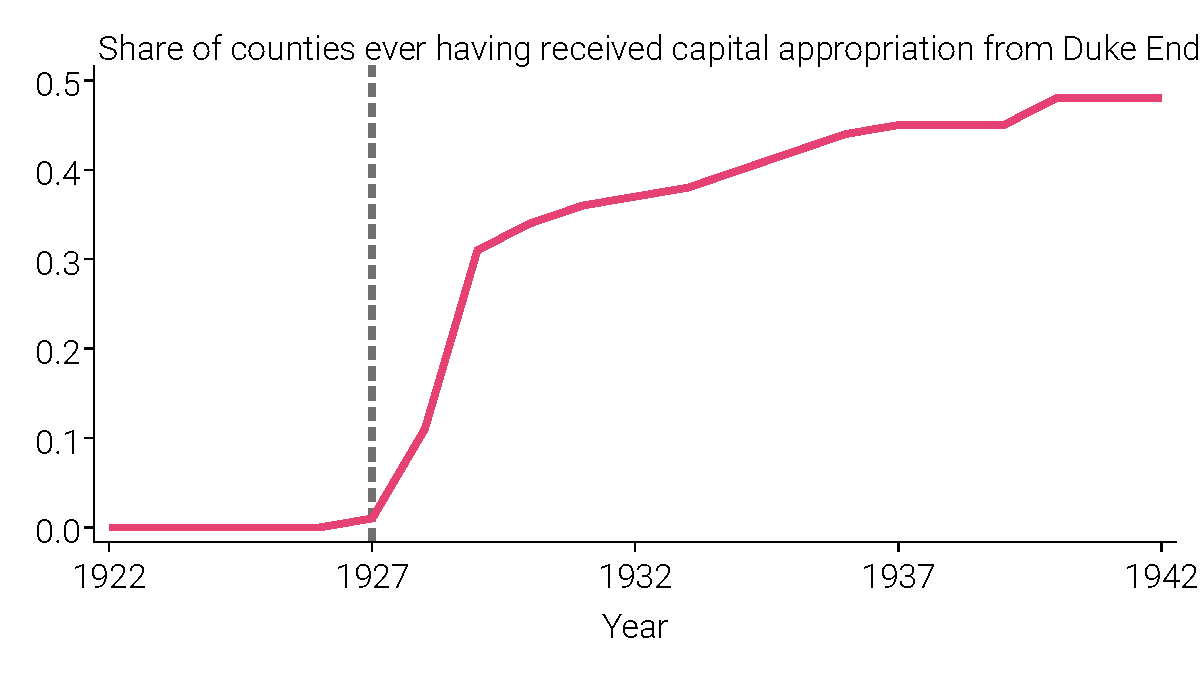
\includegraphics[width=0.8\linewidth]{../analysis/output/main/figure_1a_share_counties_treated.pdf}
        \caption[Share of counties treated by a given year]{Share of counties treated by a given year}
        \label{fig:share-counties-treated-by-year}
    \end{subfigure}
    \begin{subfigure}{\linewidth}
      \centering
      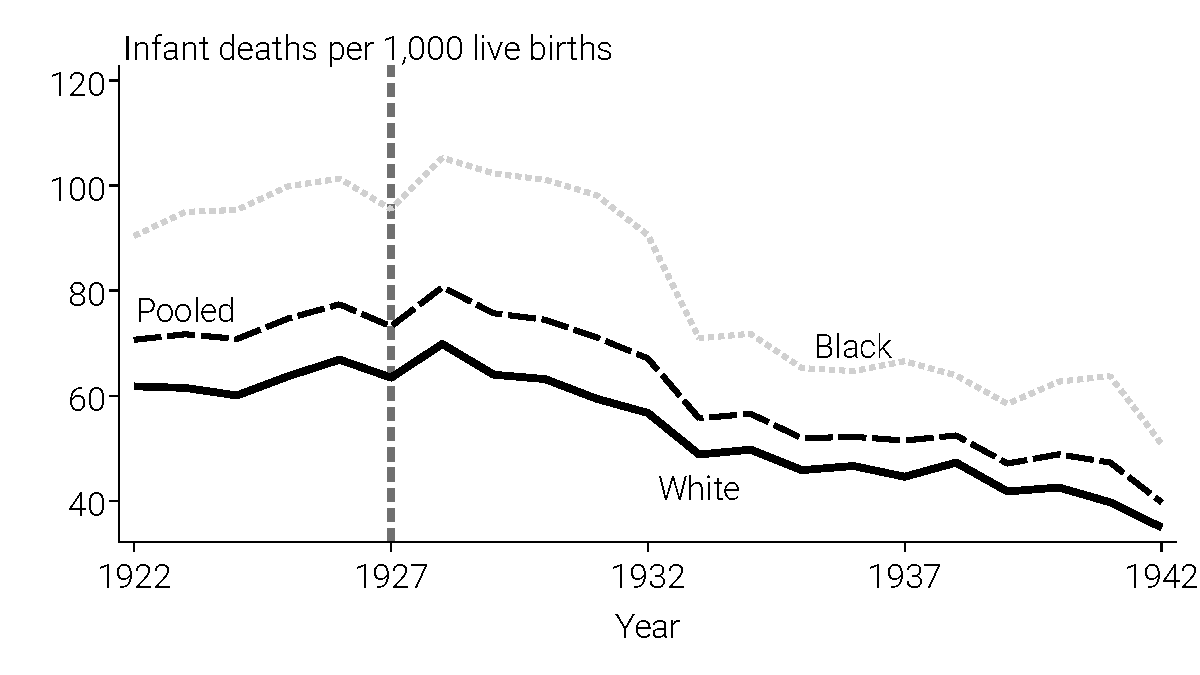
\includegraphics[width=0.8\linewidth]{../analysis/output/main/figure_1c_infant_morality_by_race_over_time.pdf}
      \caption[Infant mortality rate by year and race]{Infant mortality rate by year and race}
      \label{fig:plot-imr-race-year}
  \end{subfigure}

  \end{minipage}
  \begin{minipage}{.48\linewidth}

    \begin{subfigure}{\linewidth}
      \centering
      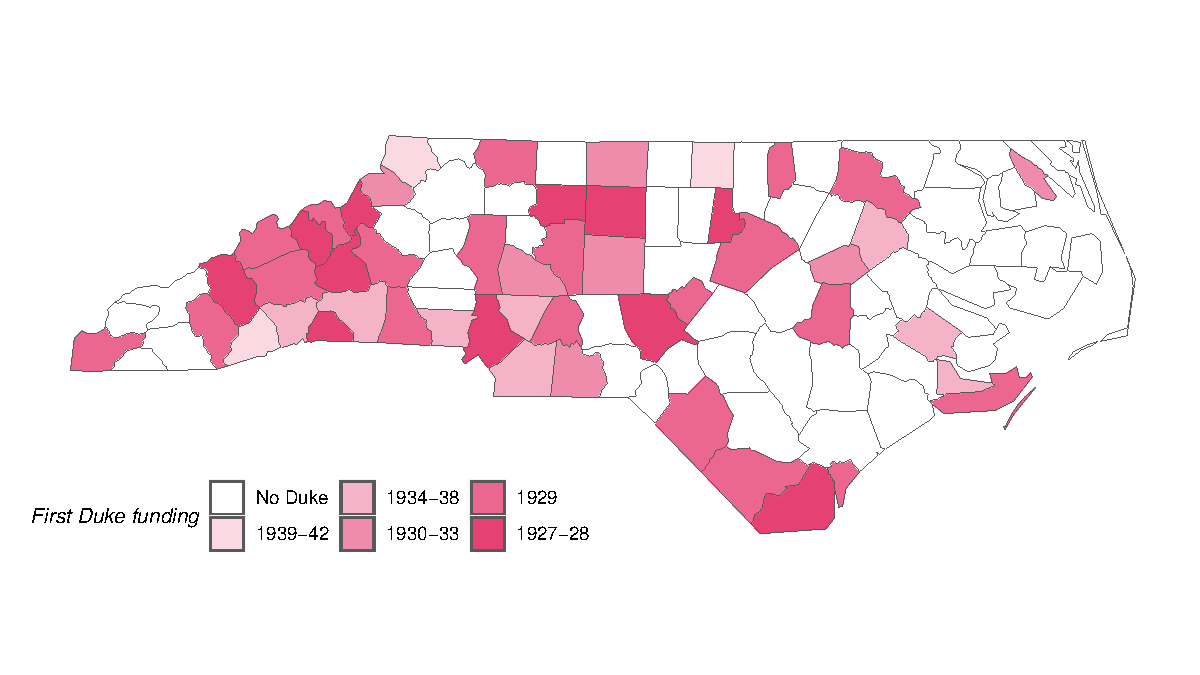
\includegraphics[width=0.72\linewidth]{../analysis/output/main/figure_1b_duke_map.pdf}
      \caption[Duration of exposure to Duke support by county]{Duration of exposure to Duke support by county}
      \label{fig:map-duke-duration}
  \end{subfigure}
    
    \begin{subfigure}{\linewidth}
        \centering
        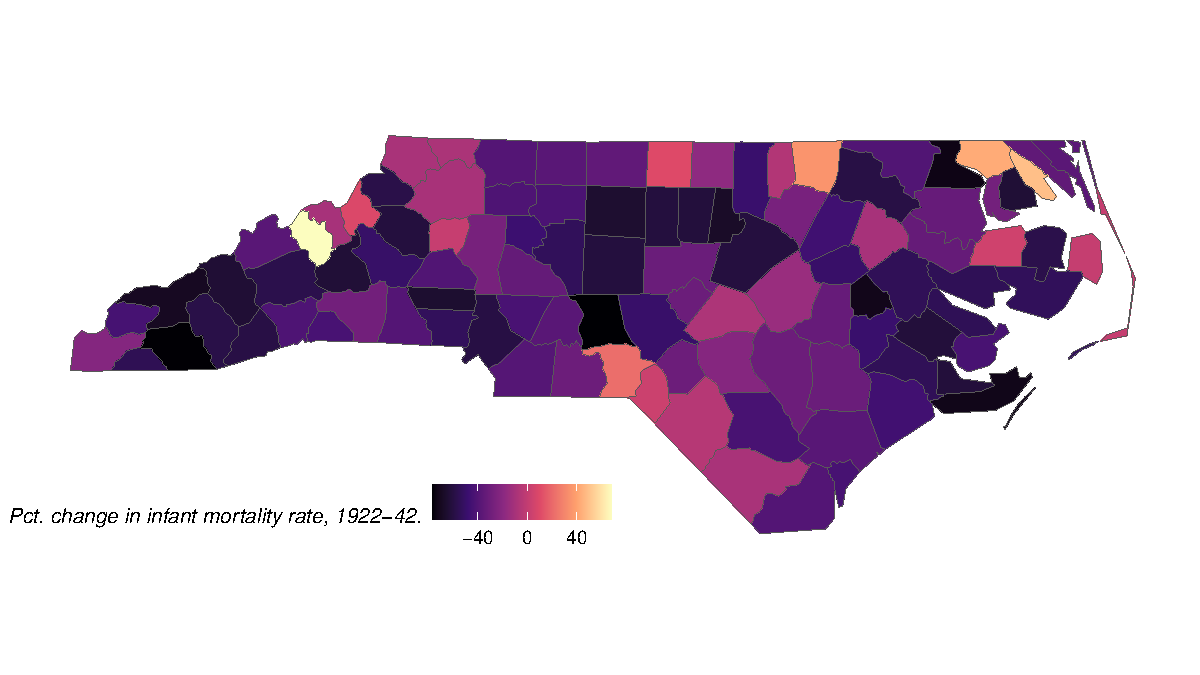
\includegraphics[width=0.72\linewidth]{../analysis/output/main/figure_1d_imr_map.pdf}
        \caption[Change in infant mortality rate, 1922-1942]{Change in infant mortality rate, 1922-1942}
        \label{fig:map-change-imr}
    \end{subfigure}
  \end{minipage}

    \label{fig:compare-roll-out-imr-changes}
    \FnoteScript{
        \scriptsize{
          Figure~\ref{fig:share-counties-treated-by-year} plots the fraction of ever-treated counties in North Carolina by calendar year.
        	Figure~\ref{fig:map-duke-duration} shows a map of county boundaries for the 100 counties in the state of North Carolina.
        	The color gradient provides a visualization of the time variation in the rollout of funding from The Duke Endowment.
        	Counties are assigned to one of five groups based on the initial year in which they received funding (dark to light red): 1927-28, 1929, 1930-33, 1934-38, 1939-42.
        	Darker counties were exposed to funding for a longer period of time.
        	Counties that did not receive funding from The Duke Endowment during the sample period from 1922 to 1942 are colored white.
        	Treatment is measured by appropriations for capital expenditures from The Duke Endowment.
        	Treatment timing is based on the \textit{Annual Report of the Hospital Section} for the years 1927 to 1942, published by The Duke Endowment.
        	Figure~\ref{fig:plot-imr-race-year} plots the average annual infant mortality rate per 1,000 live births in North Carolina between 1922 to 1942, weighted by county population, for Black infants (gray dotted line), White infants (solid black line), as well as Black and White infants pooled together (dashed black line).
          Figure~\ref{fig:map-change-imr} plots the percent change in the infant mortality rate per 1,000 live births in each North Carolina county between 1922 and 1942.
          Darker colors imply declines in infant mortality while brighter colors imply increases in infant mortality.
        }
    }
\end{figure}
\end{landscape}
\restoregeometry

% Figure 2 - Hospital beds first stage - Raw data + event study
\newgeometry{top = 0.5in, bottom = 0.5in, right = 0.5in, left = 0.5in, footskip = 0.0in}
\begin{landscape}
\begin{figure}
    \caption[Hospital beds by treatment status, ownership, and event time.]{Hospital beds at the county-level by treatment status, ownership, and event time.}
    \centering
    \begin{minipage}{\linewidth}
    \begin{subfigure}[b]{0.29\columnwidth}
        \centering
        \caption{{All general beds}}\label{fig:hosp-beds-all}
        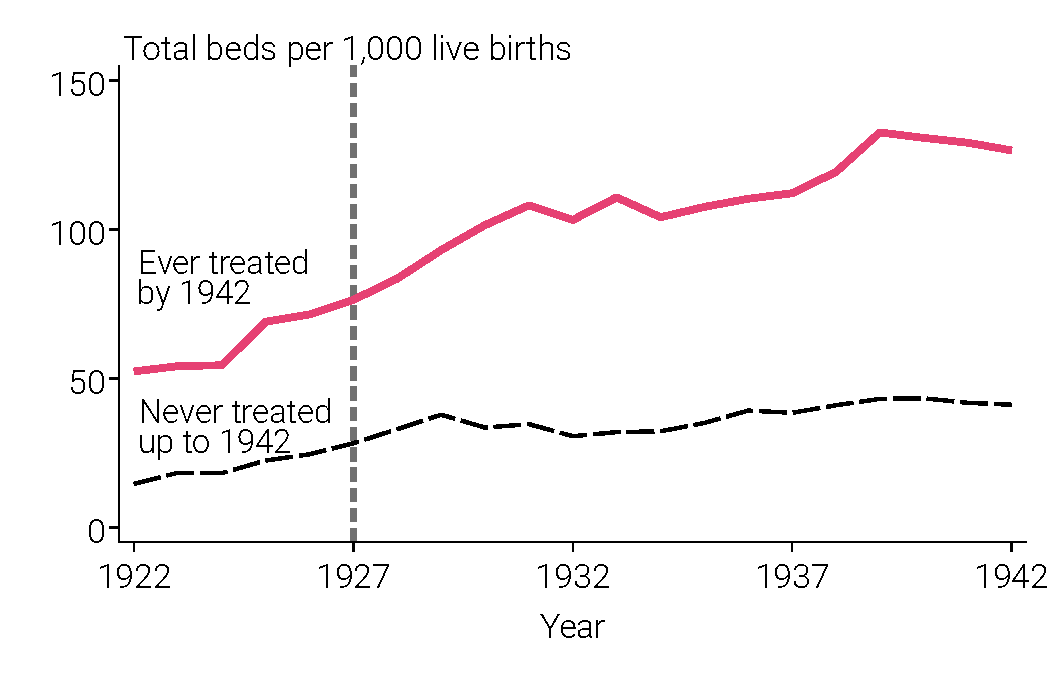
\includegraphics[width=\linewidth]{../analysis/output/main/figure_2a1_total_beds_by_year.pdf}
        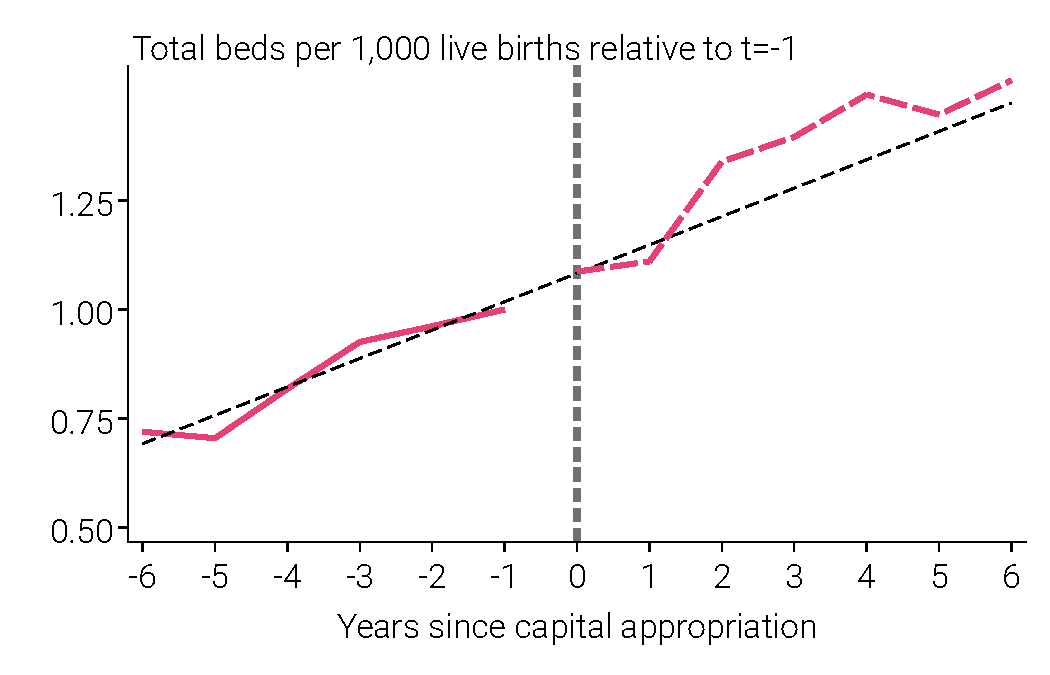
\includegraphics[width=\linewidth]{../analysis/output/main/figure_2a2_total_beds_by_event_time.pdf}
        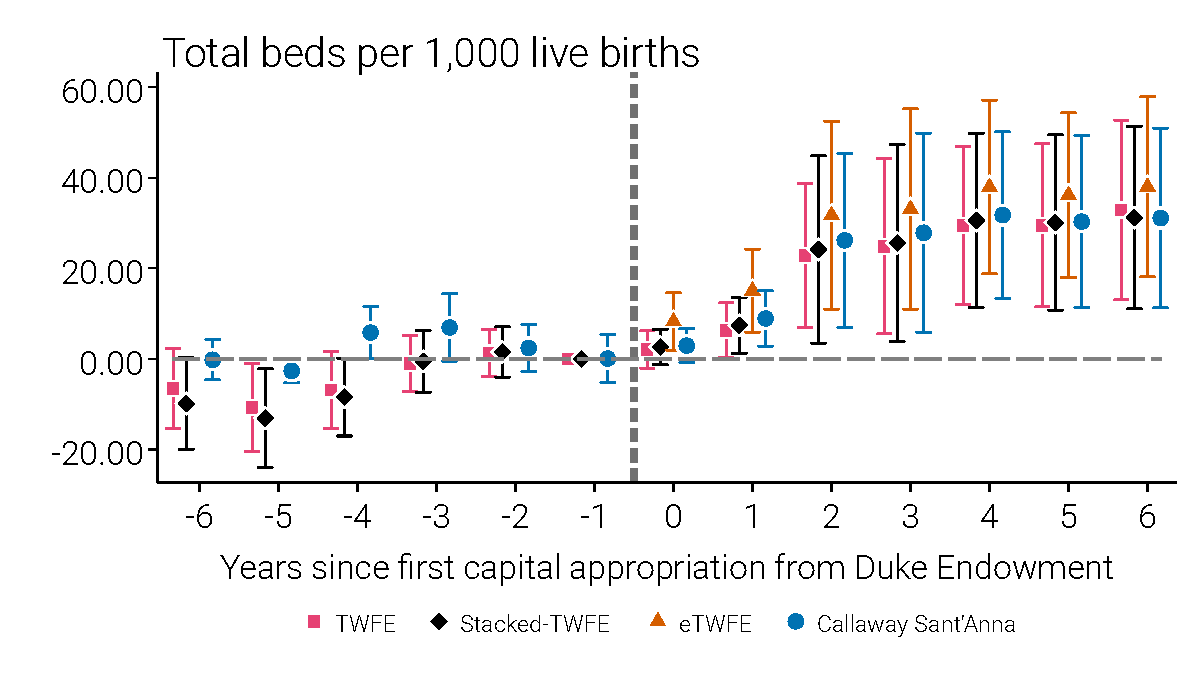
\includegraphics[width=\linewidth]{../analysis/output/main/figure_2a3_total_beds_first_stage.pdf}
    \end{subfigure}
    \hfill %%
    \begin{subfigure}[b]{0.29\textwidth}
        \centering
        \caption{{Non-profit/public/church general beds}}\label{fig:hosp-beds-likely}
        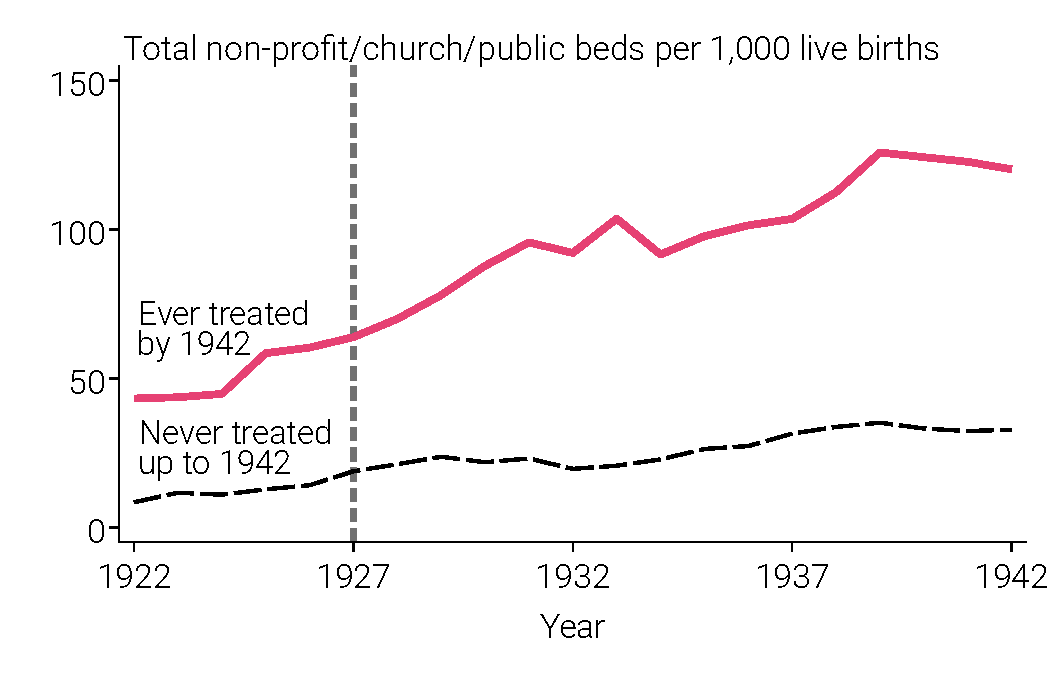
\includegraphics[width=\linewidth]{../analysis/output/main/figure_2b1_likely_beds_by_year.pdf}
        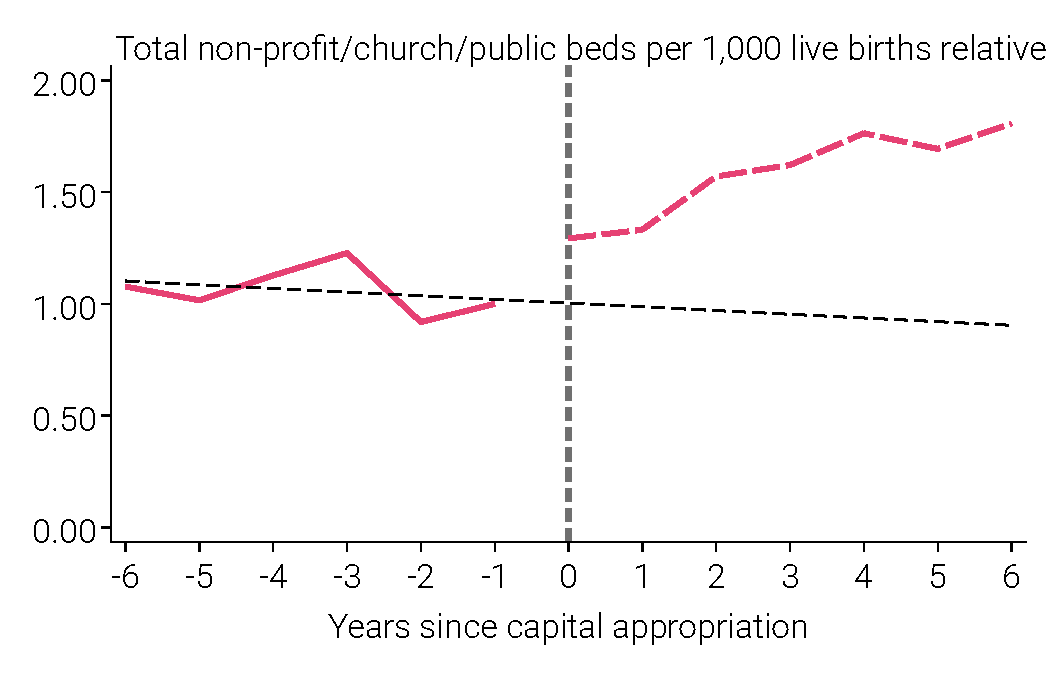
\includegraphics[width=\linewidth]{../analysis/output/main/figure_2b2_likely_beds_by_event_time.pdf}
        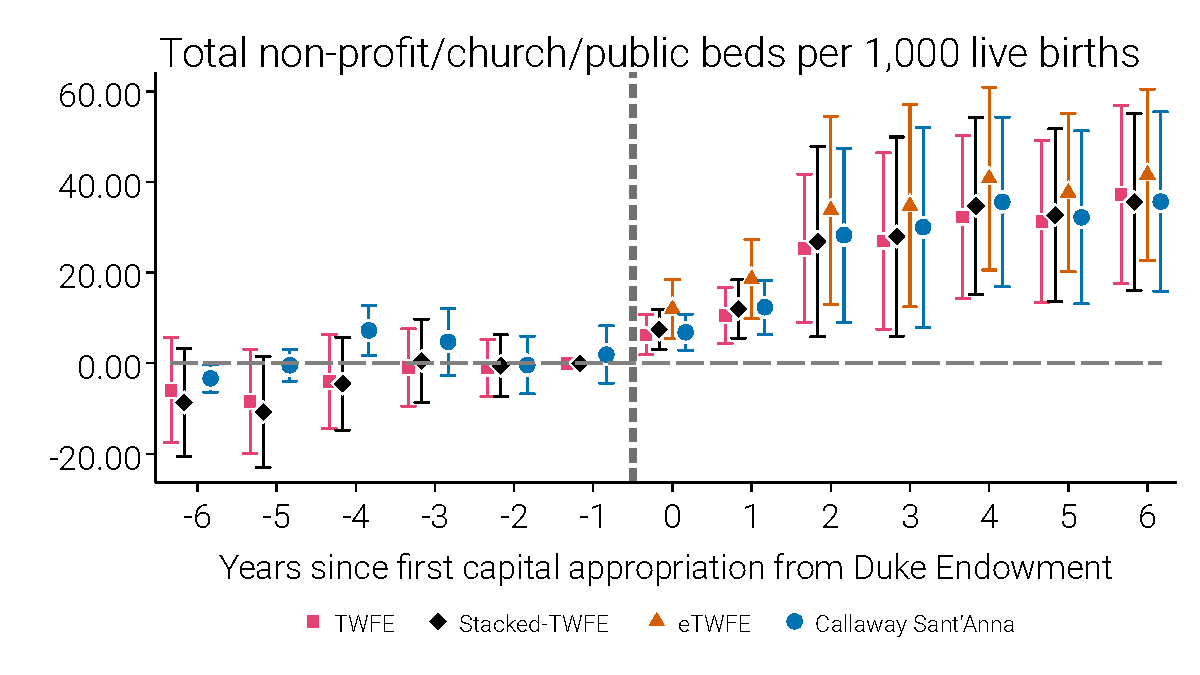
\includegraphics[width=\linewidth]{../analysis/output/main/figure_2b3_likely_beds_first_stage.pdf}
    \end{subfigure}
    \hfill %%
    \begin{subfigure}[b]{0.29\textwidth}
        \centering
        \caption{{Proprietary general beds}}\label{fig:hosp-beds-prop}
        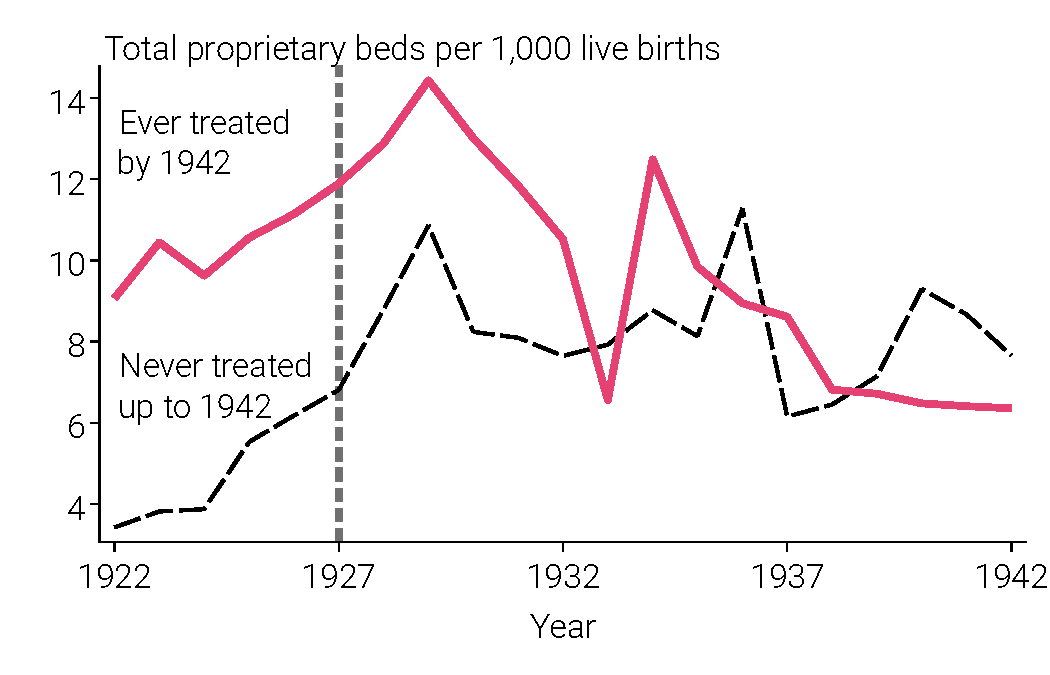
\includegraphics[width=\linewidth]{../analysis/output/main/figure_2c1_private_beds_by_year.pdf}
        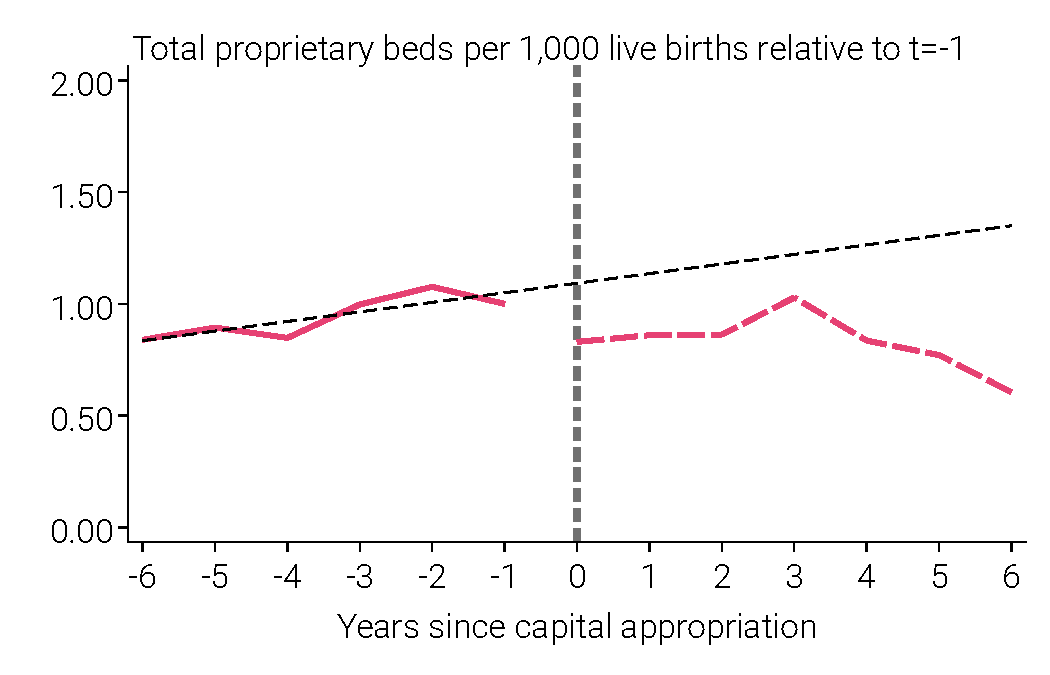
\includegraphics[width=\linewidth]{../analysis/output/main/figure_2c2_private_beds_by_event_time.pdf}
        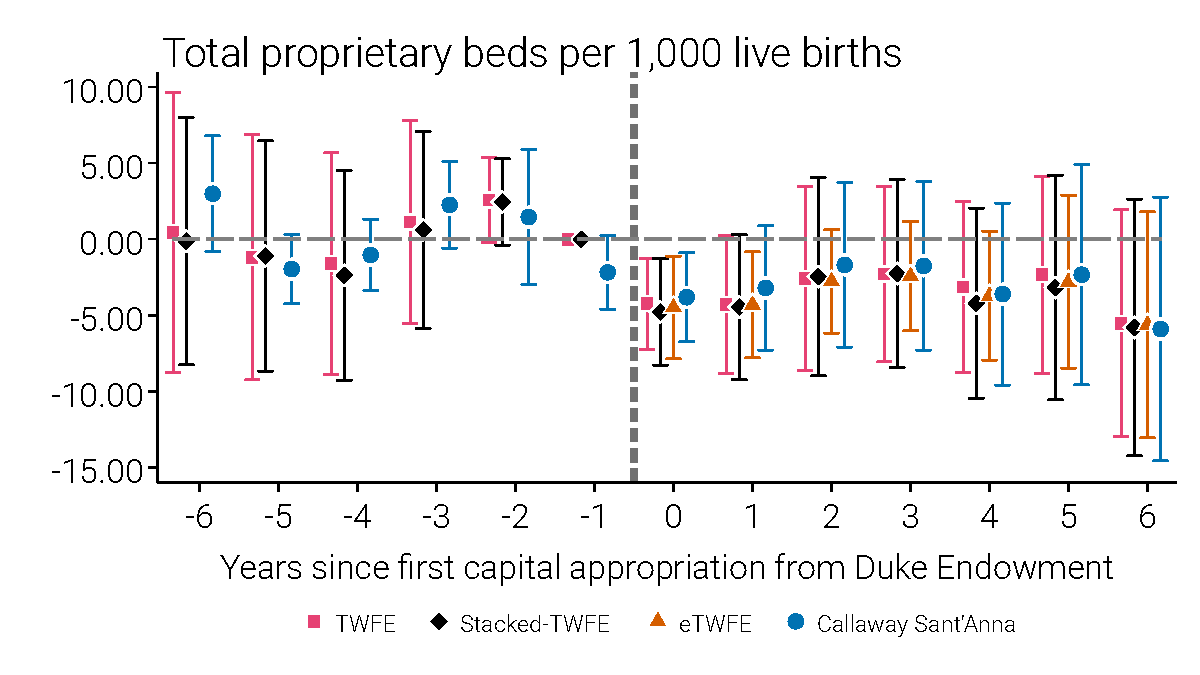
\includegraphics[width=\linewidth]{../analysis/output/main/figure_2c3_private_beds_first_stage.pdf}
    \end{subfigure}
    \end{minipage}
    \FnoteScript{
    \scriptsize{
        Column (a) plots results for the number of beds per 1,000 live births in all general hospital, column (b) plots the number of beds  per 1,000 live births in non-profit, public, or church-run general hospitals, and column (c) plots the number of beds  per 1,000 live births in proprietary general hospitals. 
        The top row of plots shows the average annual number of general hospital beds in a county by Duke treatment status.
        Counties ``Ever treated by 1942'' first received Duke funding during the sample period, between 1927 and 1942, while counties ``Never treated up to 1942'' did not.
	The middle row plots the number of general hospital beds relative to the year prior to treatment in counties treated by 1942. 
	The black dashed line is a best-fit line estimated using only pre-treatment data for treated counties.
	This trend is continued into post-treatment event time to serve as comparison to actual outcomes.
	The last row plots event study estimates of coefficient values and 95\% confidence intervals for the lead and lag indicator variables for relative time periods from $t = -6$ to $t = 6$ around the first year that a county received an appropriation for capital expenditures from The Duke Endowment.
        More extreme relative time periods are estimated but not shown in the figures. 
	The omitted category is -1 year before initial treatment.
        An observational unit is a county by year cell.
        Each plot shows four event study estimators: two-way fixed effects, stacked regression,  extended two-way fixed effects \citepMain{Wooldridge2021}, and \citeMain{CS2021}. 
        All regressions include county and year fixed effects.
	Regressions are weighted by county-by-year of birth cohort size.
	Standard errors are clustered by county.
    }
    }
    \label{fig:hosp-beds}
\end{figure}
\end{landscape}
\restoregeometry 


% Figure 3 - Doctors first stage - Raw data + event study
\newpage
\newgeometry{top = 0.5in, bottom = 0.5in, right = 0.5in, left = 0.5in, footskip = 0.0in}
\begin{landscape}
\begin{figure}
    \caption[Physician supply by treatment status, quality, and event time.]{Physician supply by treatment status, quality, and event time.}
    \centering
    \begin{minipage}{\linewidth}
    \begin{subfigure}[b]{0.27\columnwidth}
        \centering
        \caption{{Pooled doctors}}\label{fig:md-pool-all}
        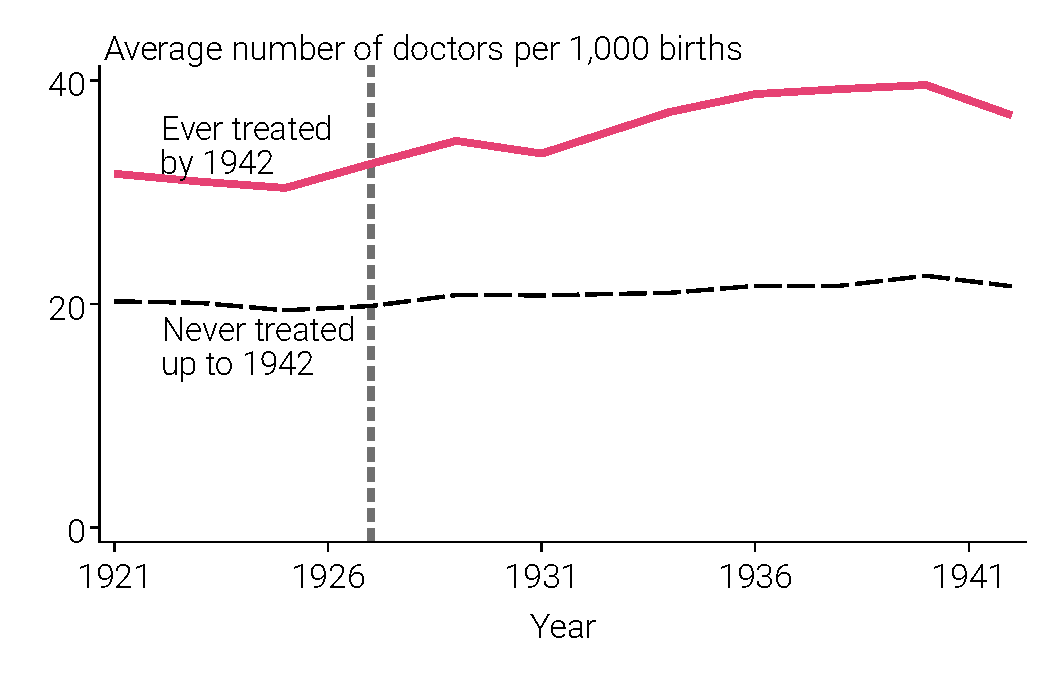
\includegraphics[width=\linewidth]{../analysis/output/main/figure_3a1_pooled_rMD_by_treat_status.pdf}
        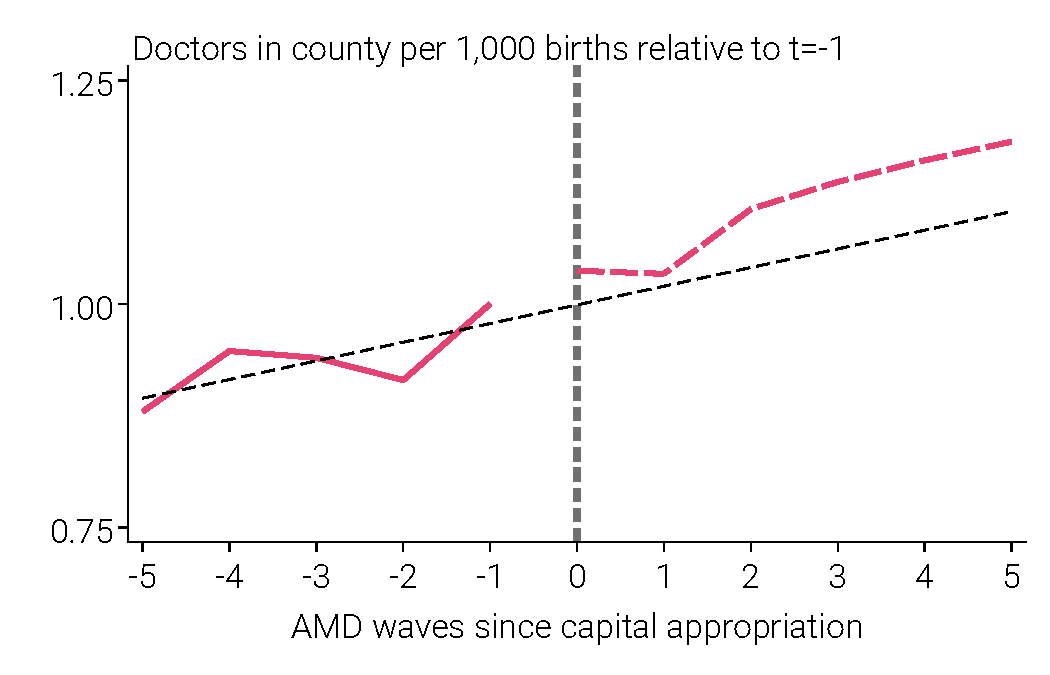
\includegraphics[width=\linewidth]{../analysis/output/main/figure_3a2_pooled_rMD_by_event_time.pdf}
        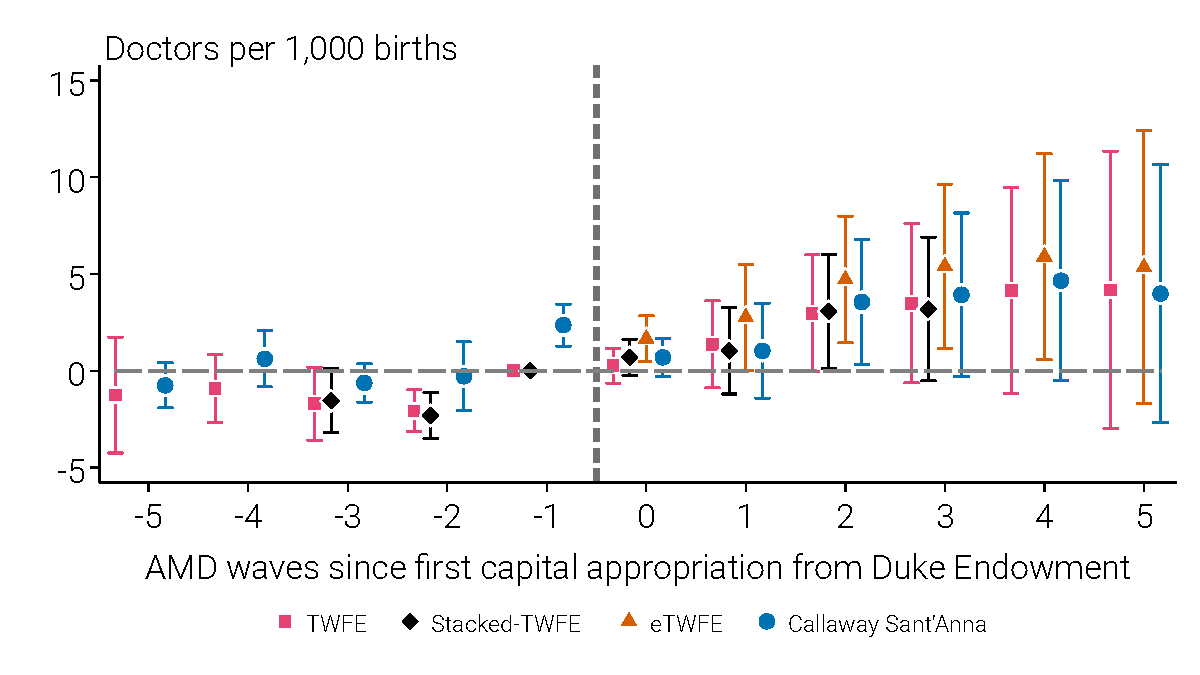
\includegraphics[width=\linewidth]{../analysis/output/main/figure_3a3_pooled_rMD_first_stage.pdf}
    \end{subfigure}
    \hfill %%
    \begin{subfigure}[b]{0.27\textwidth}
        \centering
        \caption{{Pooled high quality doctors}}\label{fig:md-pool-good}
        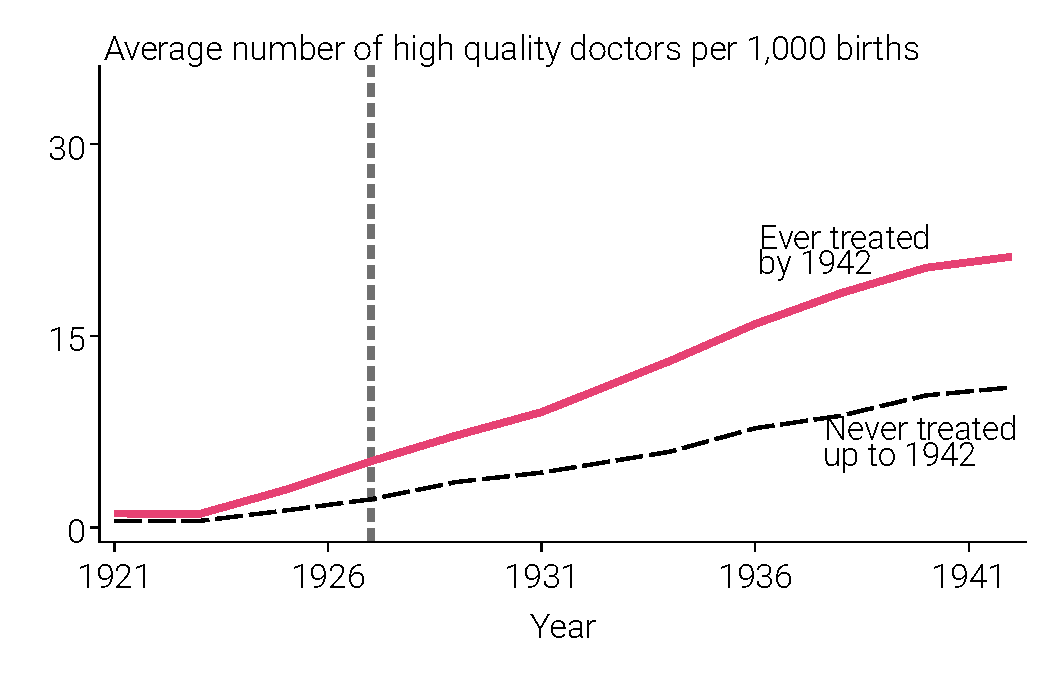
\includegraphics[width=\linewidth]{../analysis/output/main/figure_3b1_pooled_rMD_good_by_treat_status.pdf}
        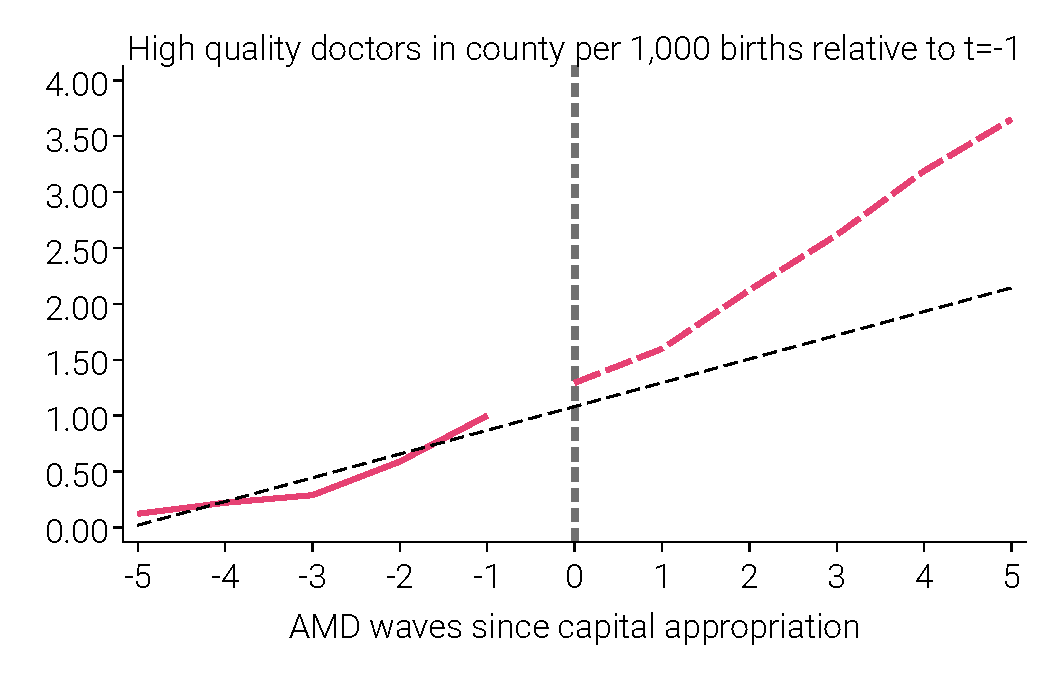
\includegraphics[width=\linewidth]{../analysis/output/main/figure_3b2_pooled_rMD_good_by_event_time.pdf}
        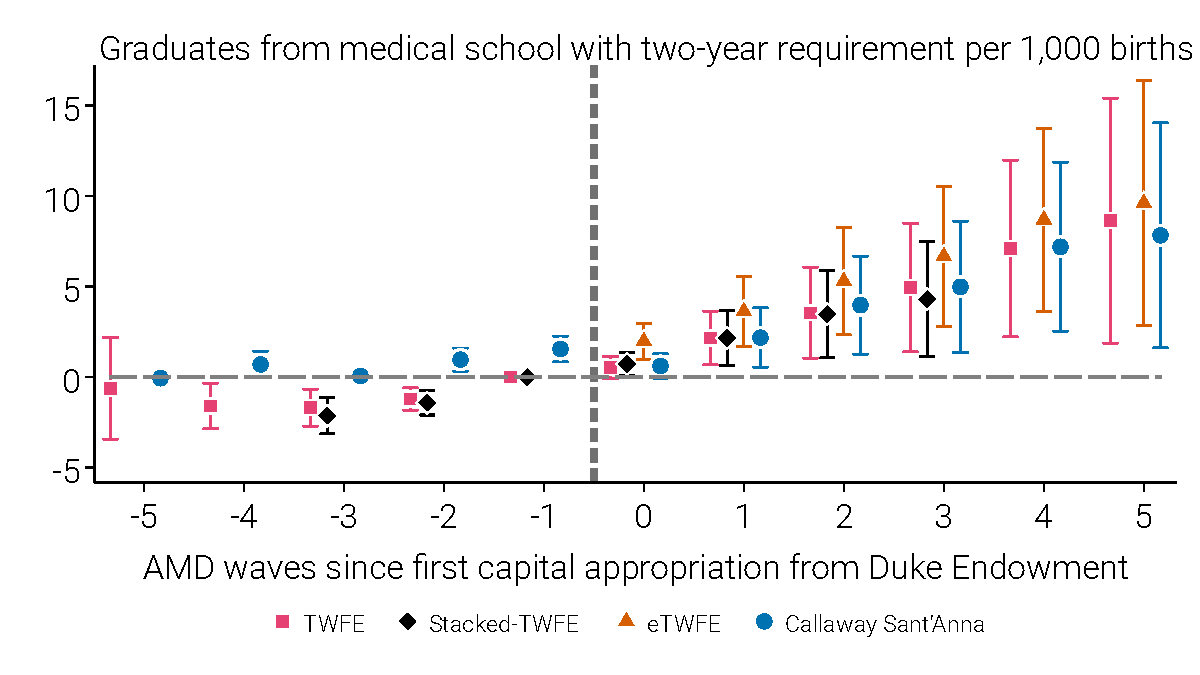
\includegraphics[width=\linewidth]{../analysis/output/main/figure_3b3_pooled_rMD_good_first_stage.pdf}
    \end{subfigure}
    \hfill %%
    \begin{subfigure}[b]{0.27\textwidth}
        \centering
        \caption{{Pooled low quality doctors}}\label{fig:md-pool-bad}
        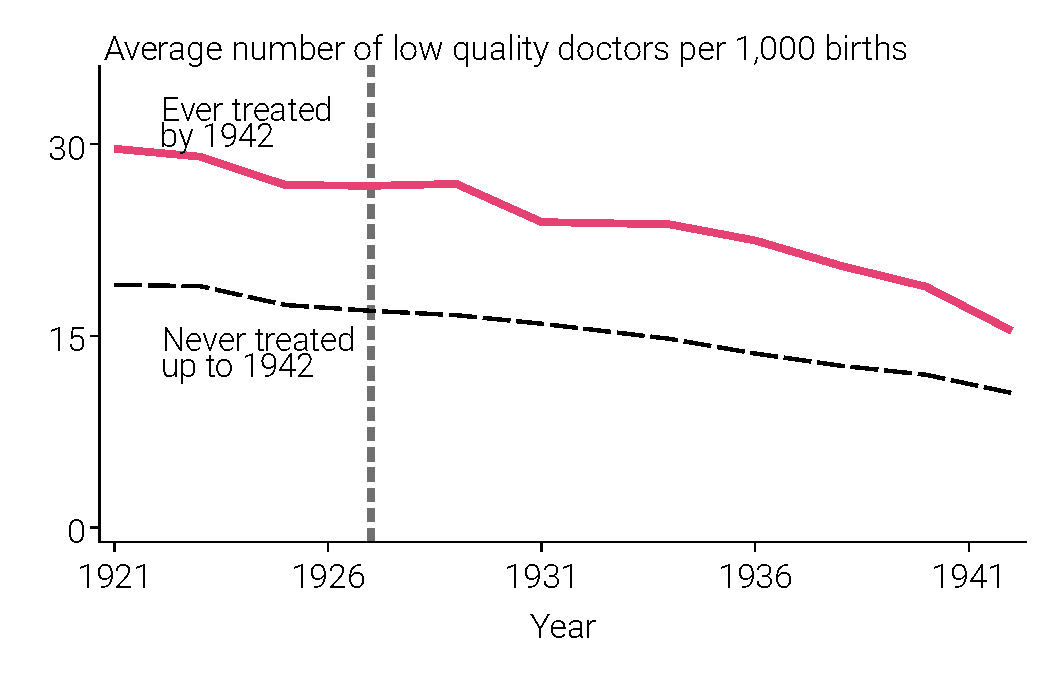
\includegraphics[width=\linewidth]{../analysis/output/main/figure_3c1_pooled_rMD_bad_by_treat_status.pdf}
        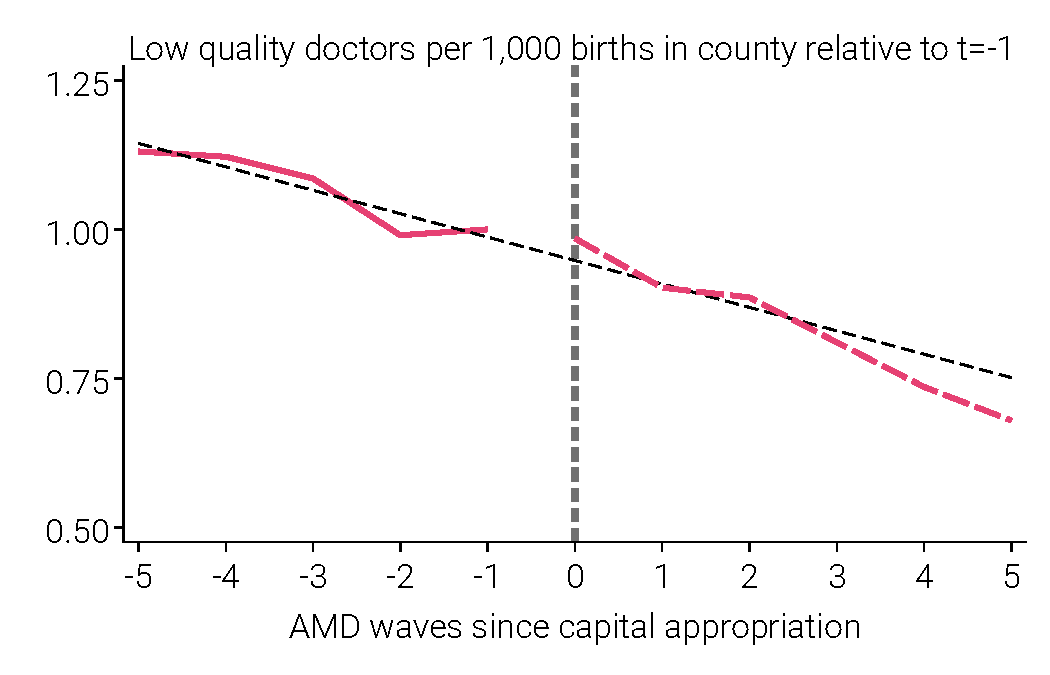
\includegraphics[width=\linewidth]{../analysis/output/main/figure_3c2_pooled_rMD_bad_by_event_time.pdf}
        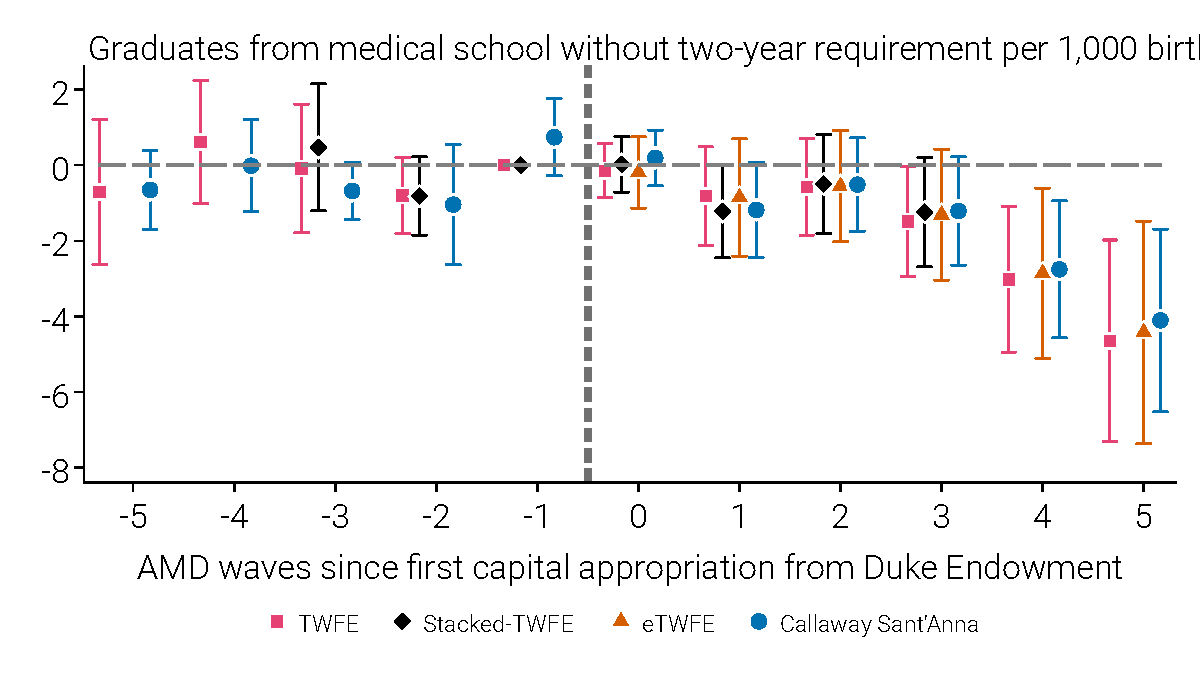
\includegraphics[width=\linewidth]{../analysis/output/main/figure_3c3_pooled_rMD_bad_first_stage.pdf}
    \end{subfigure}
    \end{minipage}
    \FnoteScript{
    \scriptsize{
        Column (a) plots results for the number of doctors, column (b) plots the number of high-quality doctors, and column (c) plots the number of low-quality doctors. 
        All columns pool doctors by race.
        A high-quality doctor is one who graduated from a medical school at least 4 years after it introduced a two-year college degree prerequisite for admission.
        All other doctors are considered low quality. 
        The top row of plots shows the average annual number of doctors in a county by Duke treatment status.
        Counties ``Ever treated by 1942'' first received Duke funding during the sample period, between 1927 and 1942, while counties ``Never treated up to 1942'' did not.
	The middle row plots the number of doctors relative to the year prior to treatment in counties treated by 1942. 
        Event time represents the number of \emph{American Medical Directory} (AMD) waves since the first year that a county received a capital appropriation from the Endowment.
        During the sample period, the AMD was published in 1921, 1923, 1925, 1927, 1929, 1931, 1934, 1936, 1938, 1940, and 1942. 
	The black dashed line is a best-fit line estimated using only pre-treatment data for treated counties.
	This trend is continued into post-treatment event time to serve as comparison to actual outcomes.
	The last row plots two-way fixed effects event study estimates of coefficient values and 95\% confidence intervals for the lead and lag indicator variables for relative time periods from $t=-5$ to $t = 5$ around the first AMD wave after a county received an appropriation for capital expenditures from The Duke Endowment (or from $t=-3$ to $t = 3$ in the case of the stacked event study).
        More extreme relative time periods are estimated but not shown in the figures. 
	The omitted category is -1 AMD wave before initial treatment.
        An observational unit is a county-by-AMD wave. 
        Each plot shows four event study estimators: two-way fixed effects, stacked regression, the extended two-way fixed effects \citepMain{Wooldridge2021}, and \citeMain{CS2021}. 
        All regressions include county and AMD-wave fixed effects.
	Regressions are weighted by county of birth cohort size averaged over the two or three years of the AMD wave.
	Standard errors are clustered by county.
    }
    }
    \label{fig:pooled-md}
\end{figure}
\end{landscape}
\restoregeometry 

% Figure 4 - Raw data by treatment status + event study DD
\newpage
\newgeometry{top = 0.5in, bottom = 0.5in, right = 0.5in, left = 0.5in, footskip = 0.0in}
\begin{landscape}
\begin{figure}
    \caption[Event study estimates and infant mortality rates by treatment status, race, and event time. Event study estimates.]{Event study estimates and infant mortality rates by treatment status, race, and event time. }
    \centering
    \begin{minipage}{\linewidth}
    \begin{subfigure}[b]{0.28\columnwidth}
        \centering
        \caption{{Pooled infant mortality rate}}\label{fig:imr-pooled}
        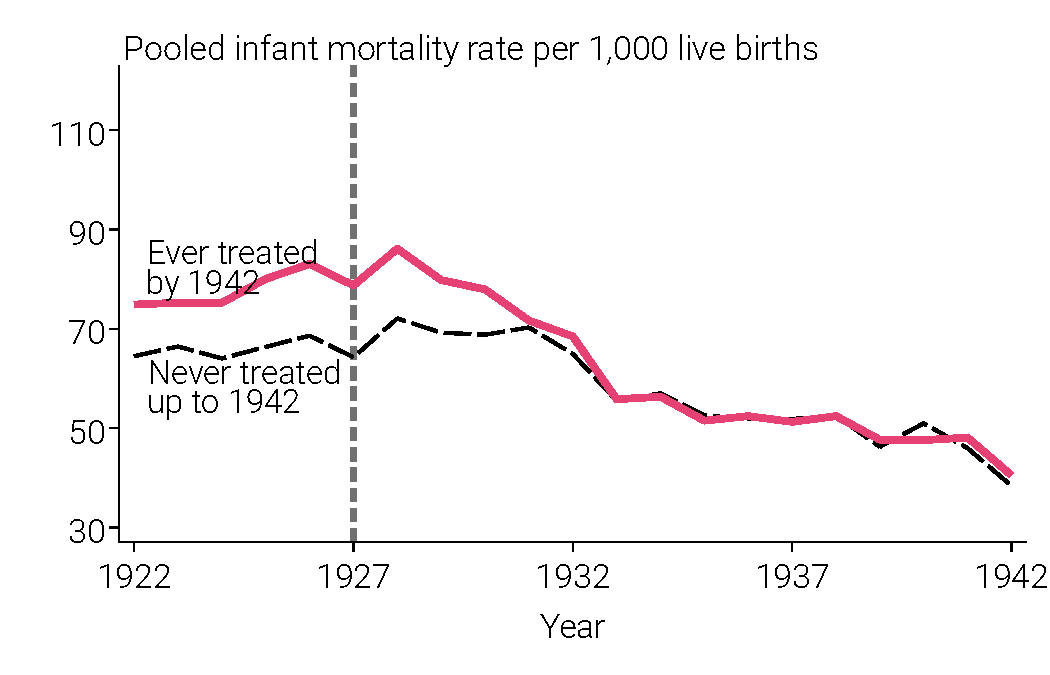
\includegraphics[width=\linewidth]{../analysis/output/main/figure_4a1_imr_by_treatment_status_pooled.pdf}
        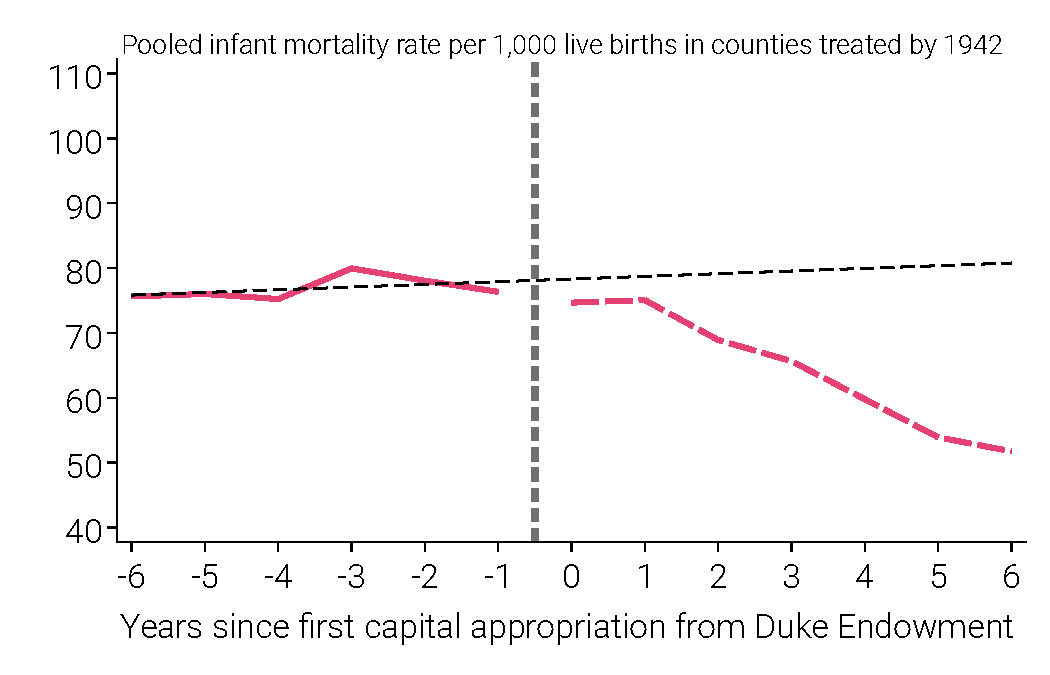
\includegraphics[width=\linewidth]{../analysis/output/main/figure_4a2_imr_by_event_time_pooled.pdf}
        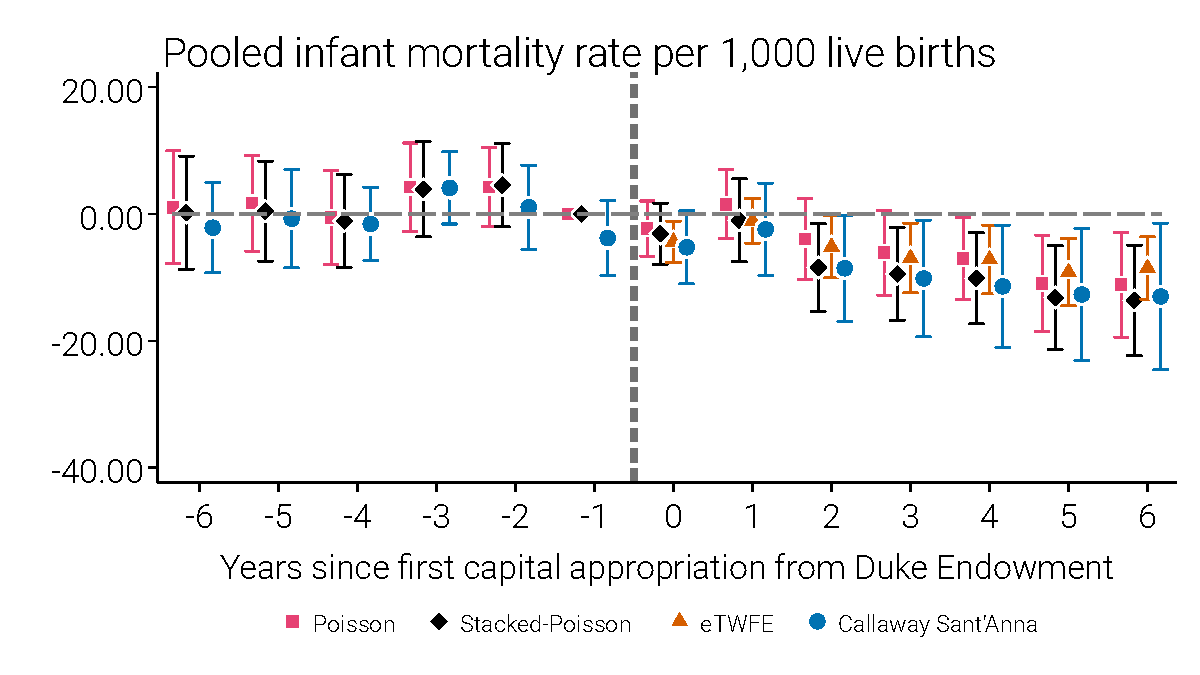
\includegraphics[width=\linewidth]{../analysis/output/main/figure_4a3_imr_event_study_pooled.pdf}
    \end{subfigure}
    \hfill %%
    \begin{subfigure}[b]{0.28\textwidth}
        \centering
        \caption{{Black infant mortality rate}}\label{fig:imr-black}
        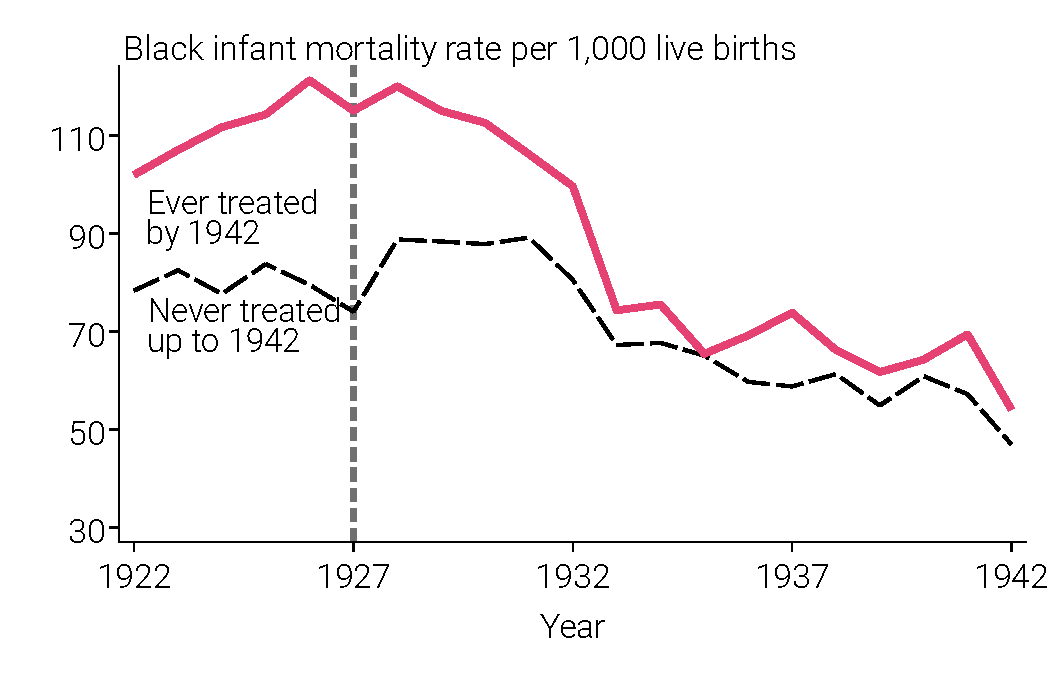
\includegraphics[width=\linewidth]{../analysis/output/main/figure_4b1_imr_by_treatment_status_black.pdf}
        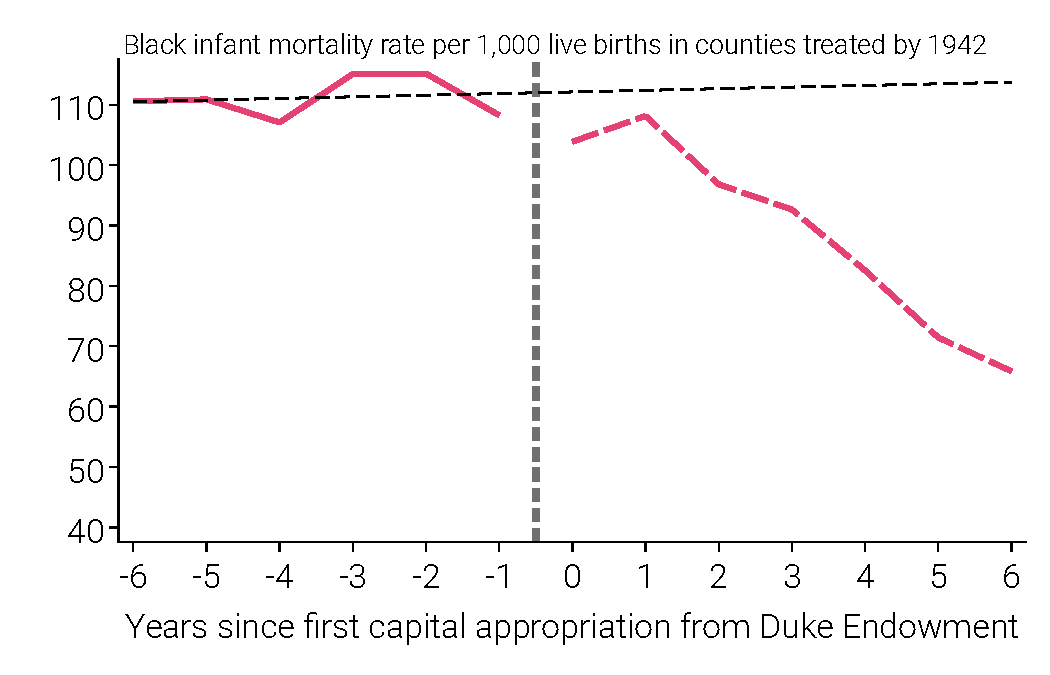
\includegraphics[width=\linewidth]{../analysis/output/main/figure_4b2_imr_by_event_time_black.pdf}
        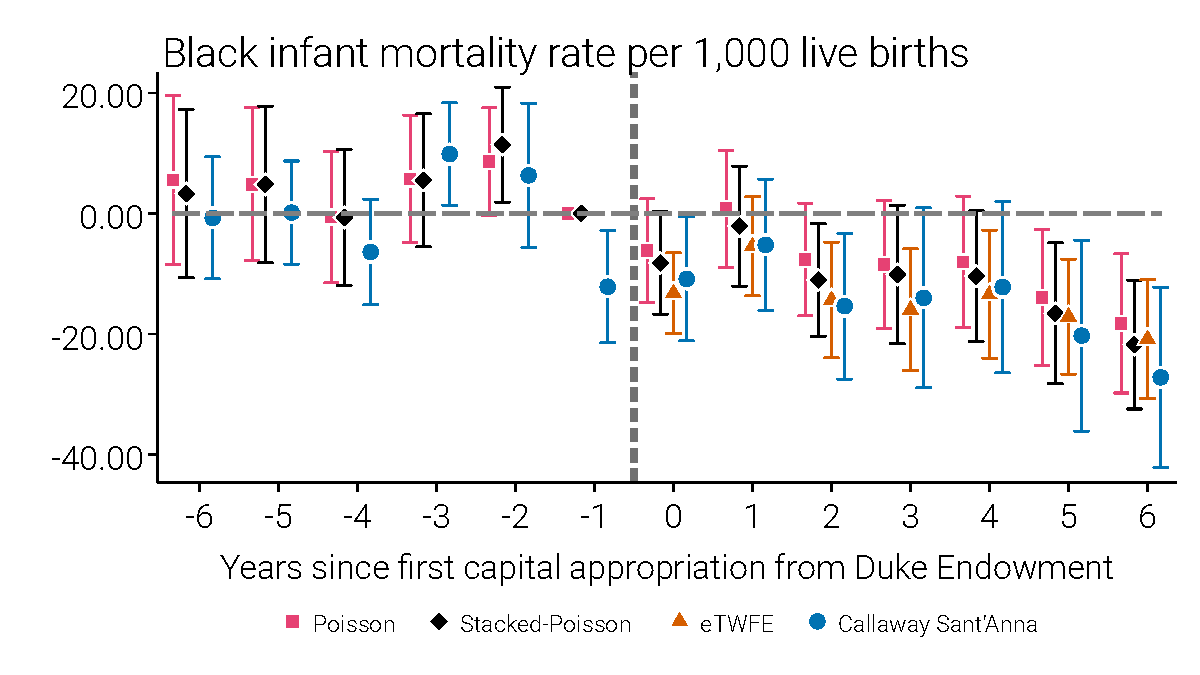
\includegraphics[width=\linewidth]{../analysis/output/main/figure_4b3_imr_event_study_black.pdf}
    \end{subfigure}
    \hfill %%
    \begin{subfigure}[b]{0.28\textwidth}
        \centering
        \caption{{White infant mortality rate}}\label{fig:imr-white}
        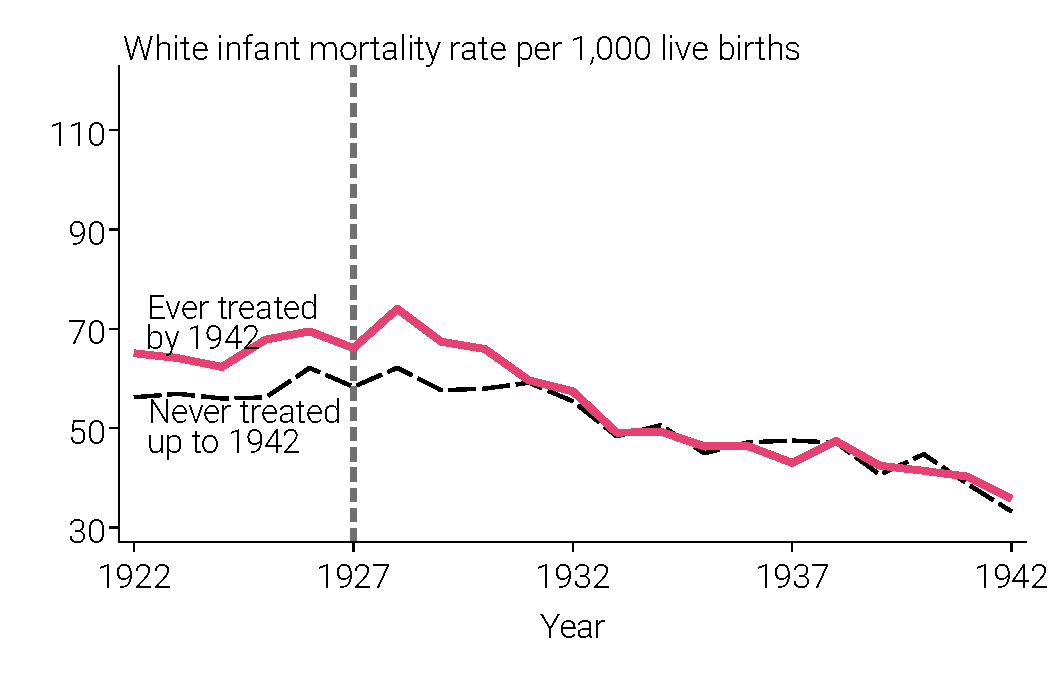
\includegraphics[width=\linewidth]{../analysis/output/main/figure_4c1_imr_by_treatment_status_white.pdf}
        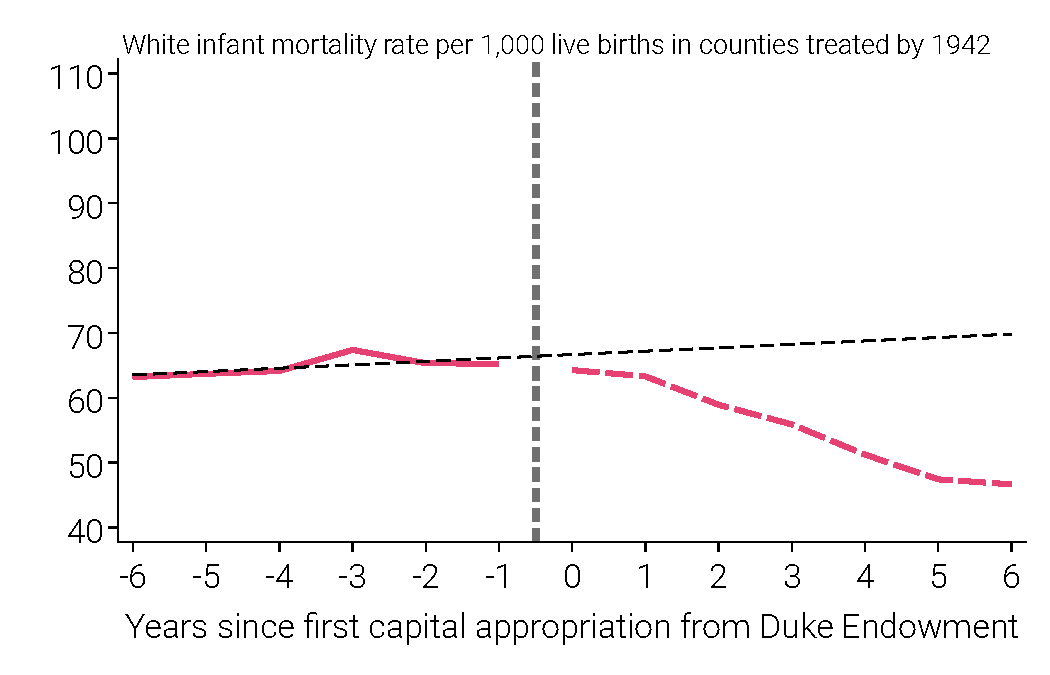
\includegraphics[width=\linewidth]{../analysis/output/main/figure_4c2_imr_by_event_time_white.pdf}
        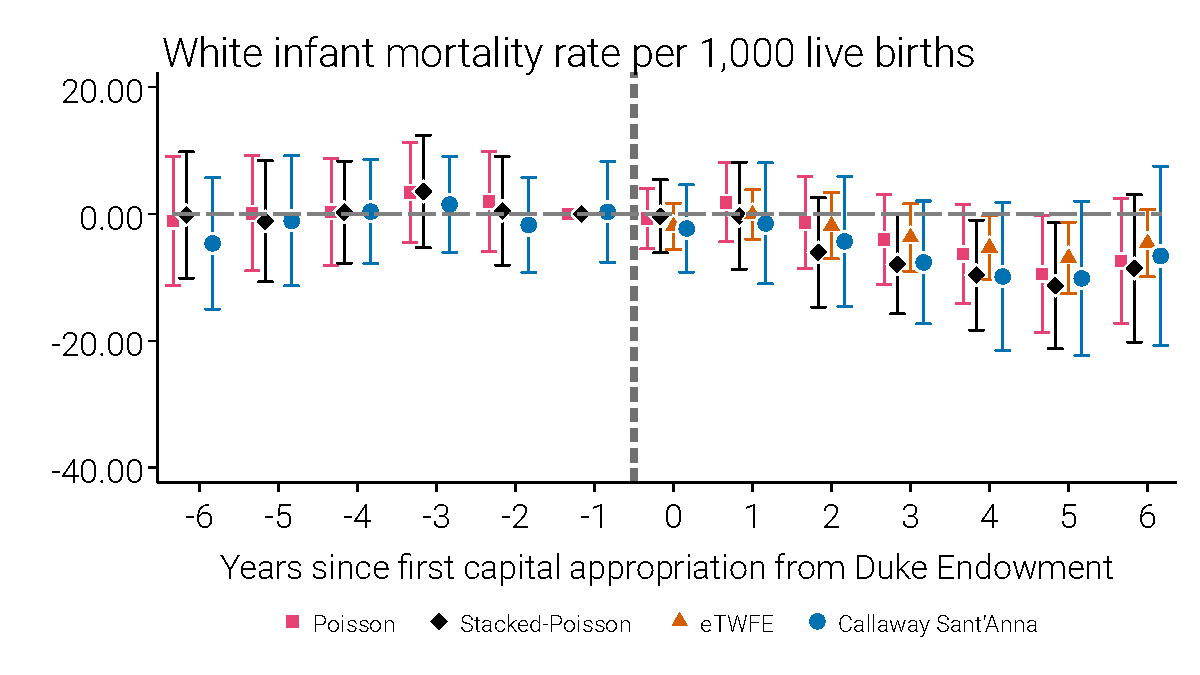
\includegraphics[width=\linewidth]{../analysis/output/main/figure_4c3_imr_event_study_white.pdf}
    \end{subfigure}
    \end{minipage}
    \label{fig:imr-raw-data-event-study}
 \FnoteScript{
 \scriptsize{
    The top row of plots shows the annual infant mortality rate per 1,000 live births by Duke treatment status for Blacks and Whites pooled together, Blacks only, and Whites only, respectively.
    Counties ``Ever treated by 1942'' first received Duke funding during the sample period, between 1927 and 1942, while counties ``Never treated up to 1942'' did not.
	The middle row plots the infant mortality rate per 1,000 live births in counties treated by 1942 in event time relative to the first year of receiving a capital appropriation from the Endowment for the same three respective groups as in the top row.
	The black dashed line is a best-fit line estimated using only pre-treatment data for treated counties.
	This trend is continued into post-treatment event time to serve as comparison to actual outcomes.
	The last row plots Poisson pseudo maximum likelihood regression estimates of exponentiated coefficient values and 95\% confidence intervals for the lead and lag indicator variables for time periods from $t=-6$ to $t=6$ around the first year that a county received an appropriation for capital expenditures from The Duke Endowment.
	Our event study plots omit the left-most coefficients for relative time periods between $-18$ and $-7$ and right-most coefficients for relative time periods between $7$ and $15$. 
	The omitted category is -1 year before initial treatment.
    An observational unit is a county-by-year birth cohort.
    Coefficients reported in the table are transformed in the following way: $100\times (exp(\beta) - 1)$.
    The dependent variables are the infant mortality rate per 1,000 live birth in birth county $c$ and year $t$: pooled by race, for Blacks only, and for Whites only, respectively.
    All regressions include county and year fixed effects.
	Regressions are weighted by county-by-year of birth cohort size.
	Standard errors are estimated using the delta method and are clustered by county of birth. }}
\end{figure}
\end{landscape}
\restoregeometry

% Figure 5 - Visual overview of robustness and appendix.
\newgeometry{left=.5in, bottom=.75in, top = .5in, right= 0.75in, footskip = 0.0in}
 \begin{figure}[!ht]
  \captionsetup[subfigure]{margin={2.0cm,0cm}}
   \hspace*{-.5cm}
    \begin{subfigure}[t]{0.495\linewidth}
      \caption{Varying specification, dependent variable, and estimator\label{fig:main-text-visual-comparison}}
      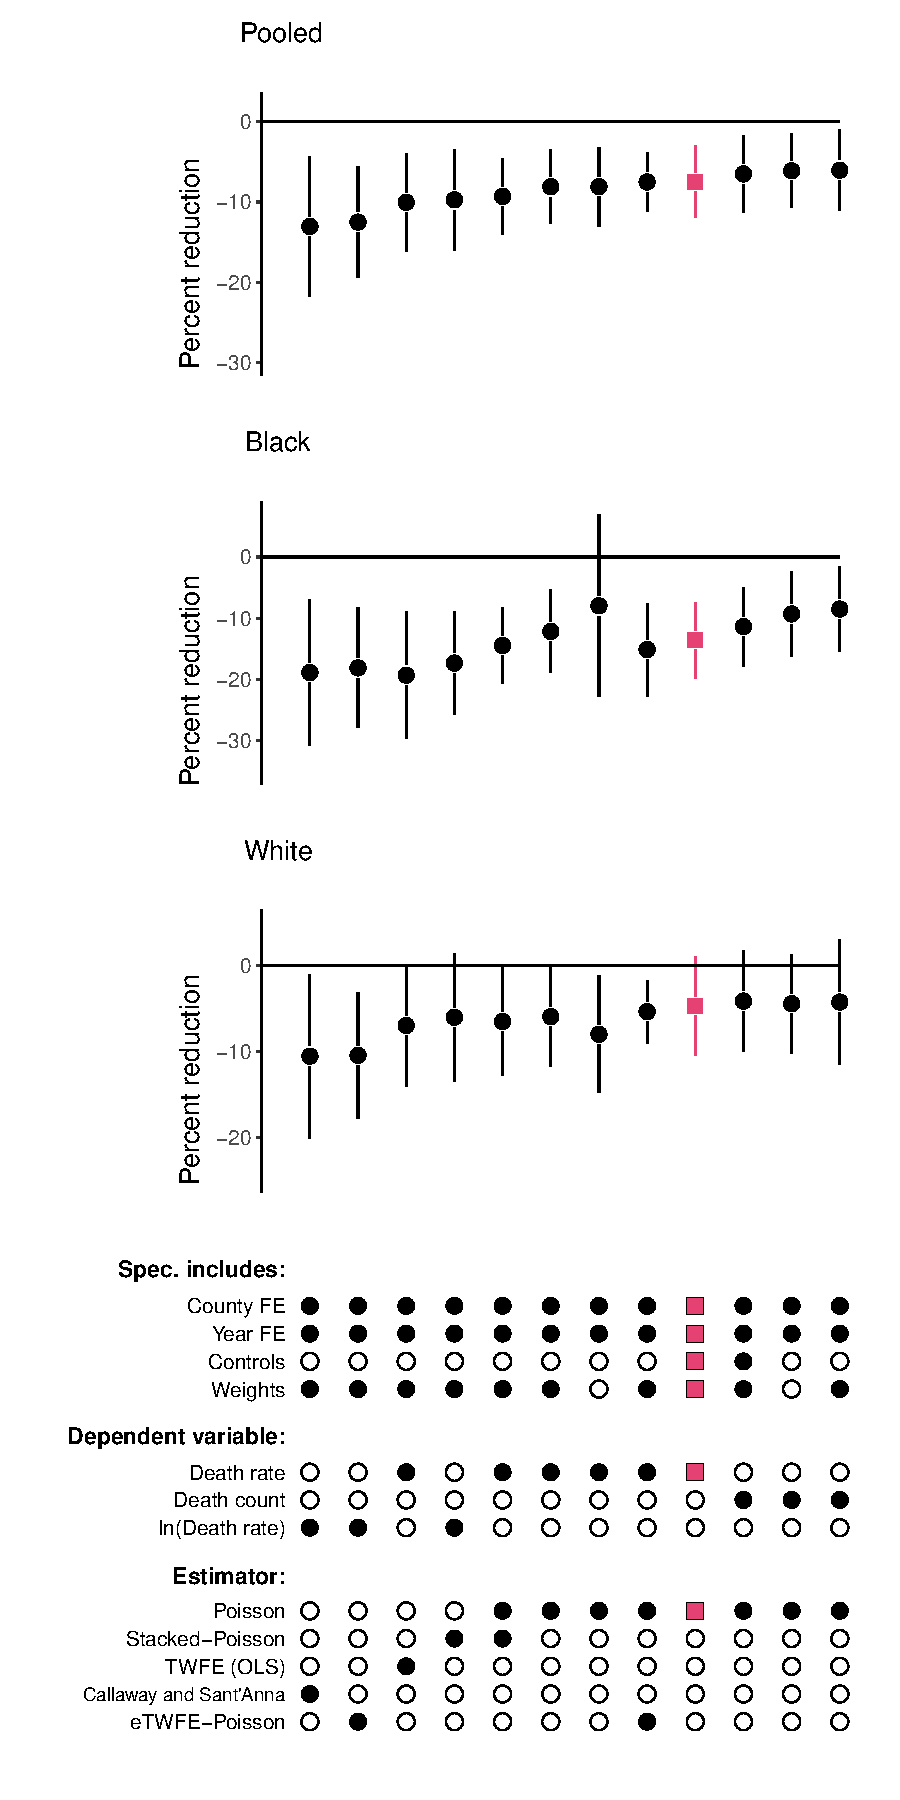
\includegraphics[width=1.0\linewidth]{../analysis/output/main/figure_5a_spec_chart_combined.pdf}
    \end{subfigure}
    \hfill
    \hspace*{-1cm}
    \begin{subfigure}[t]{0.495\linewidth}
      \caption{Varying sample for pooled infant mortality rate and preferred model\label{fig:appendix-visual-comparison}}
      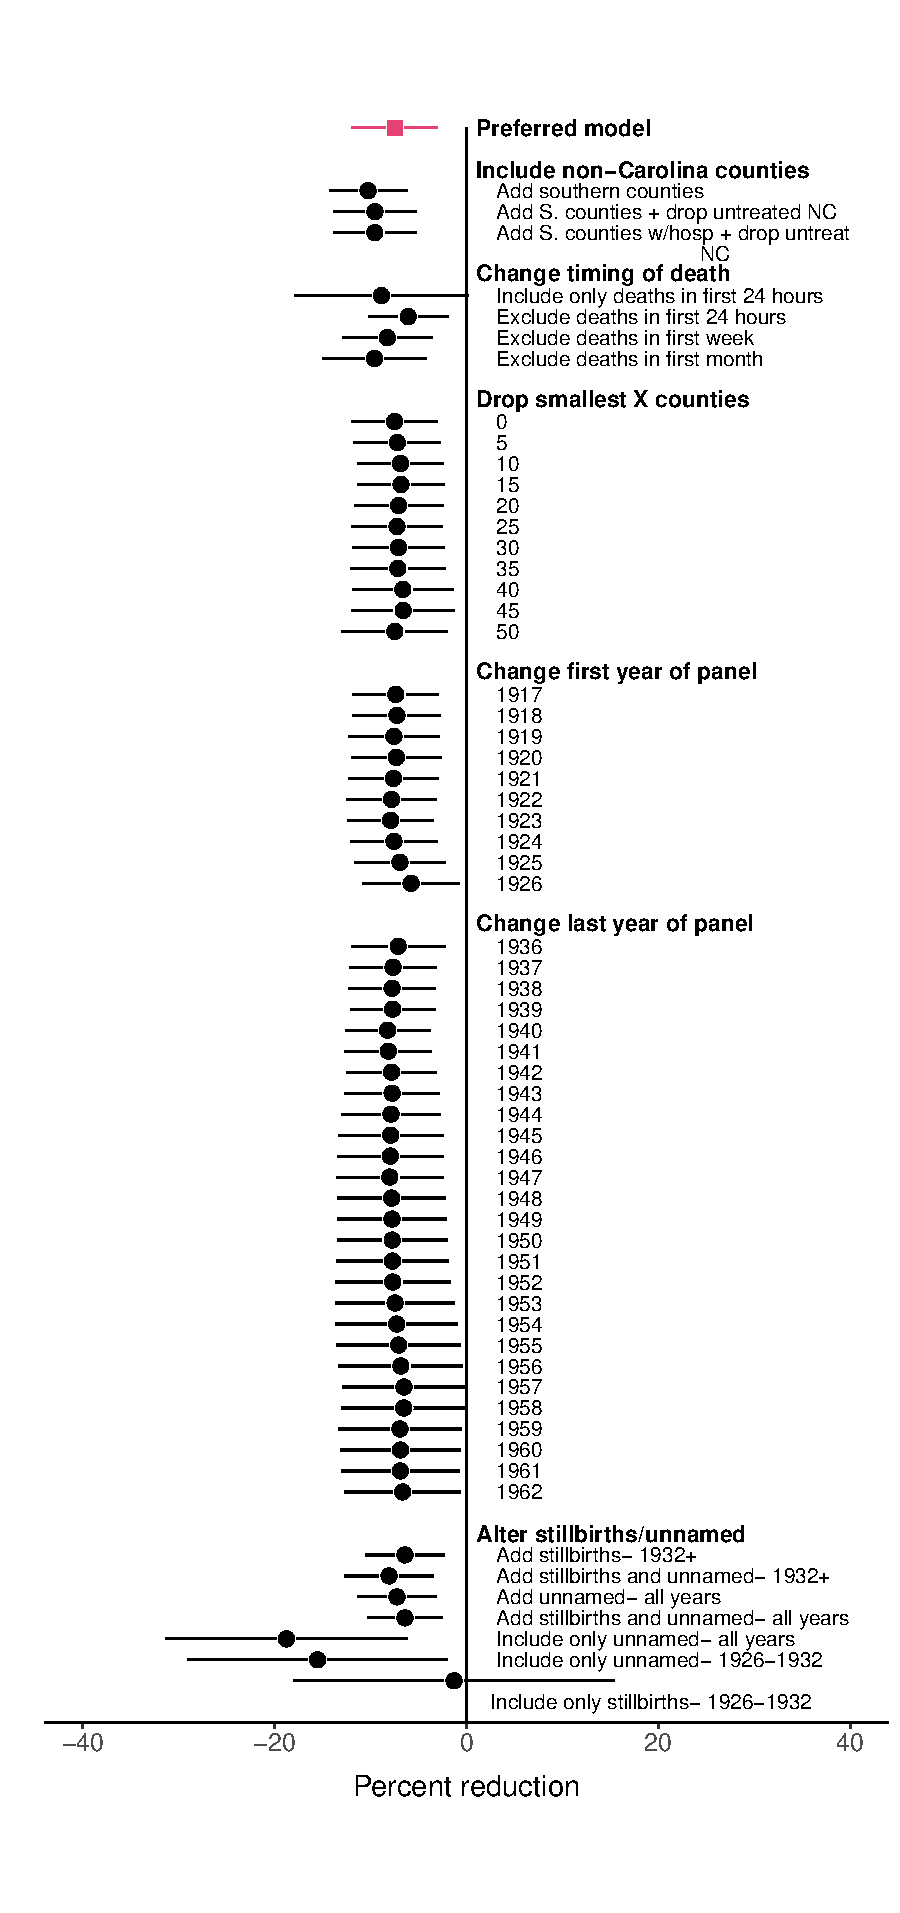
\includegraphics[width=1.0\linewidth]{../analysis/output/main/figure_5b_sample_chart.pdf}
    \end{subfigure}
    \caption{A visual representation of key robustness checks\label{fig:spec-chart}}
    \vspace{-36pt}
    \captionsetup[subfigure]{margin={0.5cm,0cm}}
    \Fnote{
    Point estimates and 95-percent confidence interval for the coefficient on Duke support.
    See Table~\ref{tab:imr-did-poisson} and Online Appendix Tables~\ref{tab:infant-mortality-alt-specs} and \ref{tab:infant-mortality-log-specs} for a description of the specifications plotted in panel A.
    See Online Appendix Tables~\ref{tab:imr-llmr-long-run-sample-southern-states}, \ref{tab:imr-did-poisson-by-timing}, and \ref{tab:robust-still-unnamed} for specifications in panel B.
    Specifications that change the first or last year of the panel use births from \citeMain{baileyCountyLevelNatalityMortality2015} in constructing the dependent variable because North Carolina Vital Statistics data are only available from 1922 to 1948.
    Estimates in panel B are based on our preferred specification from column 6 of Table~\ref{tab:imr-did-poisson}.
    Standard errors are estimated using the delta method and are clustered at the county level.
    }
  \end{figure}
\restoregeometry


%------------------------------------------%
%               Appendix
%------------------------------------------%
\appendix
\singlespacing

% Restart page count
\setcounter{page}{1}

\renewcommand*{\thepage}{A\arabic{page}}

%------------------------------------------%
%      Appendix A - Info about raw data
%------------------------------------------%

\newpage
\newgeometry{top = 0.5in, bottom = 0.5in, right = 0.75in, left = 0.75in, footskip = 0.0in}
\setcounter{table}{0}\renewcommand{\thetable}{\ref{sec:appx-images-data}\arabic{table}}
\setcounter{figure}{0}\renewcommand{\thefigure}{\ref{sec:appx-images-data}\arabic{figure}}

\FloatBarrier
\begin{center}
{\Large Online Appendix}
 ~\\ ~\\
\noindent{\large \textbf{The Gift of a Lifetime: The Hospital, Modern Medicine, and Mortality}}
 ~\\ 
\noindent Alex Hollingsworth, Krzysztof Karbownik, Melissa A. Thomasson, and Anthony Wray
\end{center}
\section[Sample images of data sources]{Sample images of data sources\label{sec:appx-images-data}}
\setcounter{table}{0}\renewcommand{\thetable}{\ref{sec:appx-images-data}\arabic{table}}
\setcounter{figure}{0}\renewcommand{\thefigure}{\ref{sec:appx-images-data}\arabic{figure}}

% Figure A1
\begin{figure}[!ht]
    \centering
    \caption[Sample images]{Sample images\label{fig:data-source-images}}
    \begin{minipage}{1.0\linewidth}
    \centering
    \begin{subfigure}[b]{1.0\textwidth}
        \centering
        \caption{The Duke Endowment's \textit{Annual Report of the Hospital Section}}
        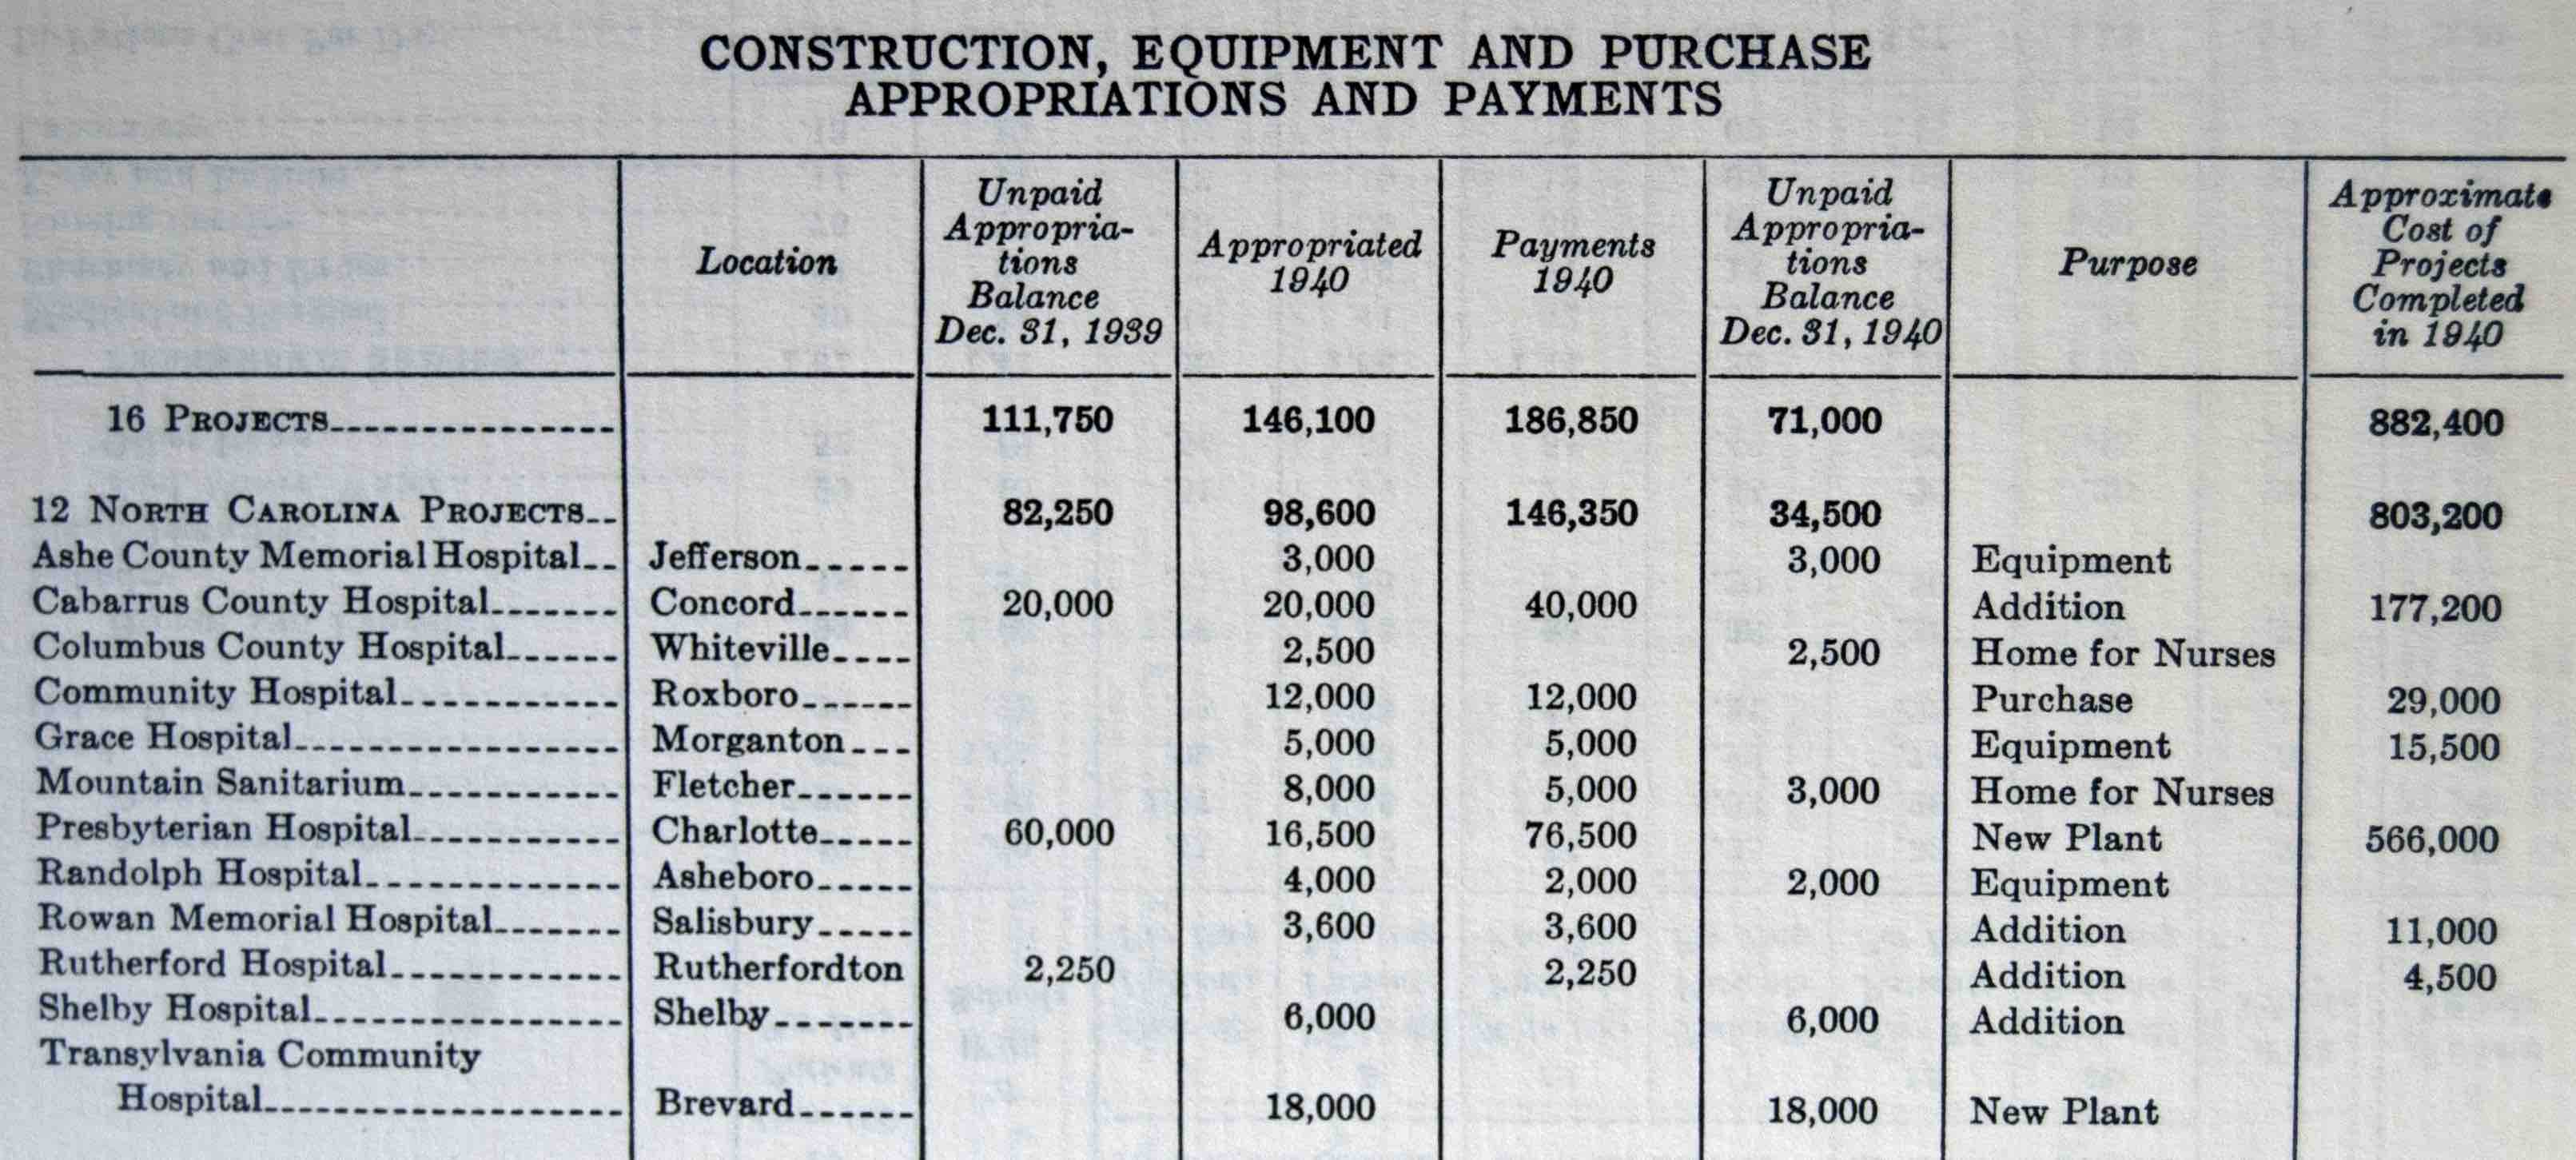
\includegraphics[width=\linewidth]{../pics/sample_image_duke_capital_ex.jpg}
    \end{subfigure}
    \vspace{12pt}
    \begin{subfigure}[b]{1.0\textwidth}
        \centering
        \caption{\textit{American Medical Directory}} % excerpt from p. 1252 of 1934 volume
        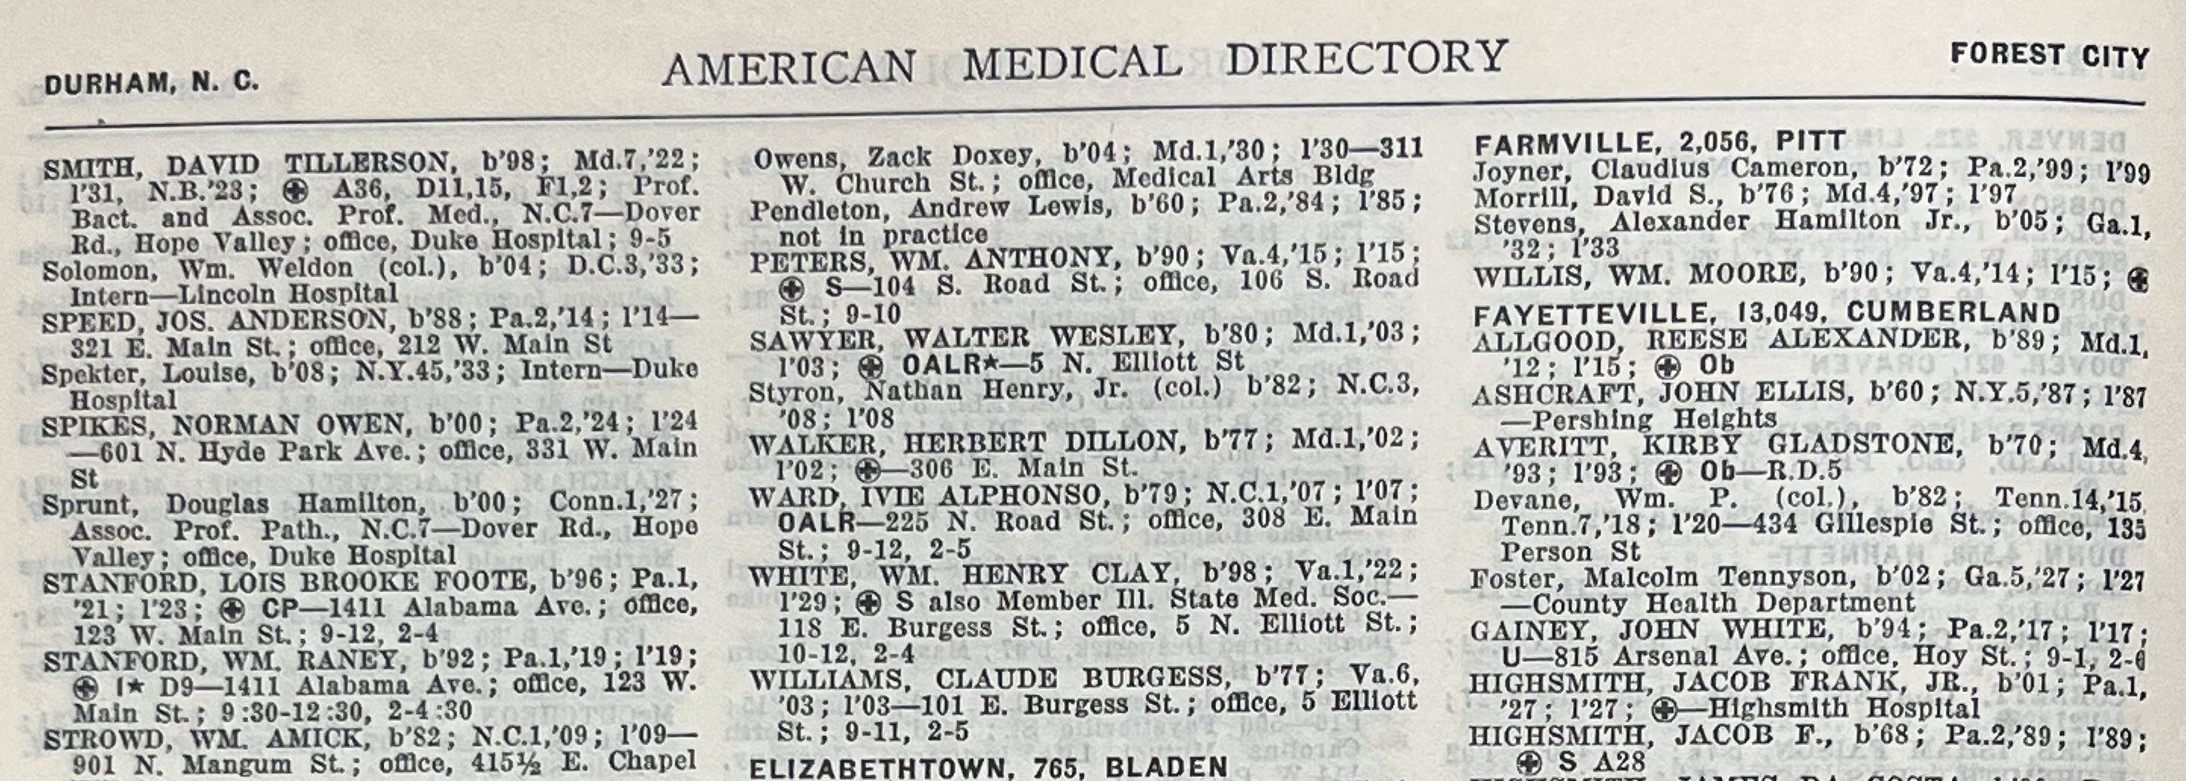
\includegraphics[width=\linewidth]{../pics/sample_image_amd_1934.jpg}
    \end{subfigure}
    \end{minipage}
    \Fnote{Example images of The Duke Endowment's \textit{Annual Report of the Hospital Section}, the source for our measure of exposure to Duke support (top) and the \textit{American Medical Directory}, the source for the number of physicians by county and year (bottom). Photo credits: Authors.}
\end{figure}
\restoregeometry


%-------------------------------------------------------------------%
%                Appendix B - Hospitals first stage - Alternate specs
%-------------------------------------------------------------------%

\FloatBarrier
\newpage
\newgeometry{top = 0.75in, bottom = 0.75in, right = 0.75in, left = 0.75in, footskip = 0.0in}
\begin{landscape}
\section{First stage for hospitals and hospital beds: Additional results \label{sec:hospitals-first-stage-robust}}
\setcounter{table}{0}\renewcommand{\thetable}{\ref{sec:hospitals-first-stage-robust}\arabic{table}}
\setcounter{figure}{0}\renewcommand{\thefigure}{\ref{sec:hospitals-first-stage-robust}\arabic{figure}}

% Table B1
\begin{table}[!ht]\centering
    \centering
    \caption{First stage for hospitals and hospital beds: Robustness to other estimators and treatment definition\label{tab:hospitals-robust-alt-specs}}
    \begin{adjustbox}{width=.95\linewidth}
    \begin{threeparttable}
        \estauto{../analysis/output/appendix/table_b1_county_level_hospitals_robustness.tex}{8}{S[table-format=2.4,table-column-width=20mm]}
        \Fignote{
            Each coefficient comes from a separate regression estimated by two-way fixed effects (columns 1 and 5), stacked regression (columns 2 and 6), extended two-way fixed effects by \citeApp{Wooldridge2021} (columns 3 and 7), or \citeApp{CS2021} (columns 4 and 8). 
            In columns 1 to 4, the dependent variable is the number of hospital beds (Panel A) or the number of hospitals (Panel B) in a county and year. 
            Within Panel A, the dependent variable is the number of beds in hospitals of any type (top row); in non-profit, church-owned, or public hospitals (middle row); or in proprietary hospitals (bottom row). 
            Panel B presents the same classification across rows with the number of hospitals of each type as the dependent variable. 
            Columns 5 to 8 express the dependent variables as rates per 1,000 live births and follows the same structure as columns 1 to 4. 
            Each coefficient represents the change in the outcome variable due to receiving a capital appropriation from The Duke Endowment. 
            In panel A the treatment includes all capital appropriations while panel B excludes homes for nurses. 
            The weights are the number of births in a county and year.
            Standard errors are clustered at the county level.
        }
    \end{threeparttable}
\end{adjustbox}
\end{table}
\end{landscape}
\restoregeometry
\renewcommand{\thefigure}{B\arabic{figure}}

% Figure B1
\newpage
\newgeometry{top = 0.5in, bottom = 0.5in, right = 0.5in, left = 0.5in, footskip = 0.0in}
\begin{figure}
  \caption[Hospitals by treatment status, ownership, and event time.]{Hospitals at the county-level by treatment status, ownership, and event time.}\label{fig:hosp-count}
  \centering
  \begin{minipage}{\linewidth}
  \begin{subfigure}[b]{0.49\columnwidth}
    \caption{\scriptsize{Descriptive}}
    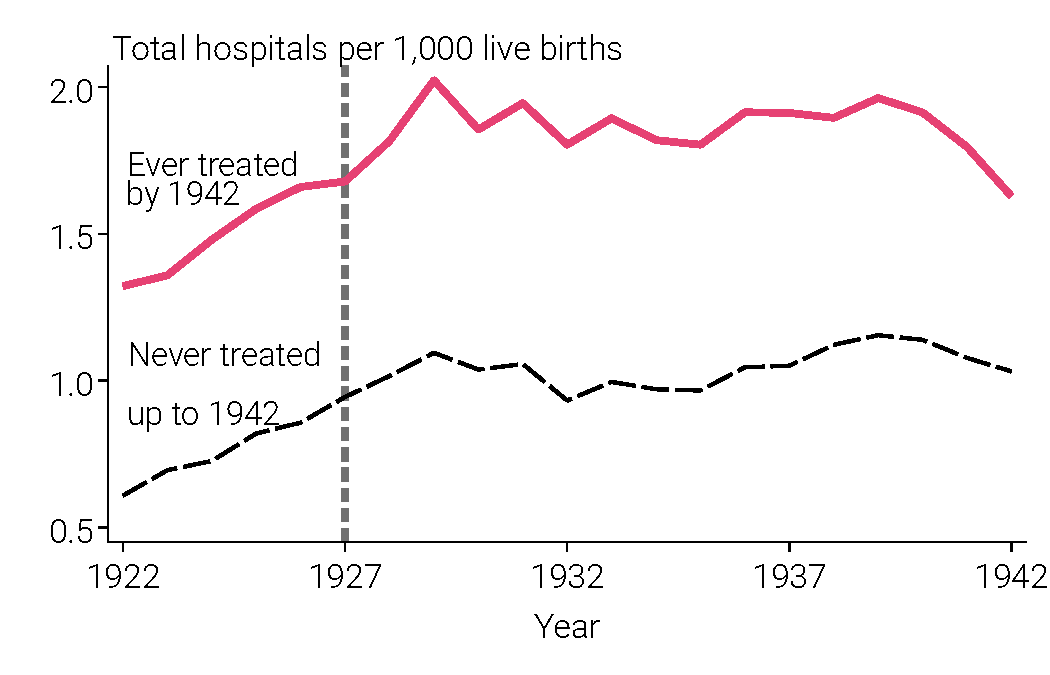
\includegraphics[width=\linewidth]{../analysis/output/appendix/figure_b1a1_total_hospitals_by_year.pdf}  \end{subfigure} 
  \begin{subfigure}[b]{0.49\columnwidth}
    \caption{\scriptsize{Event studies}}
    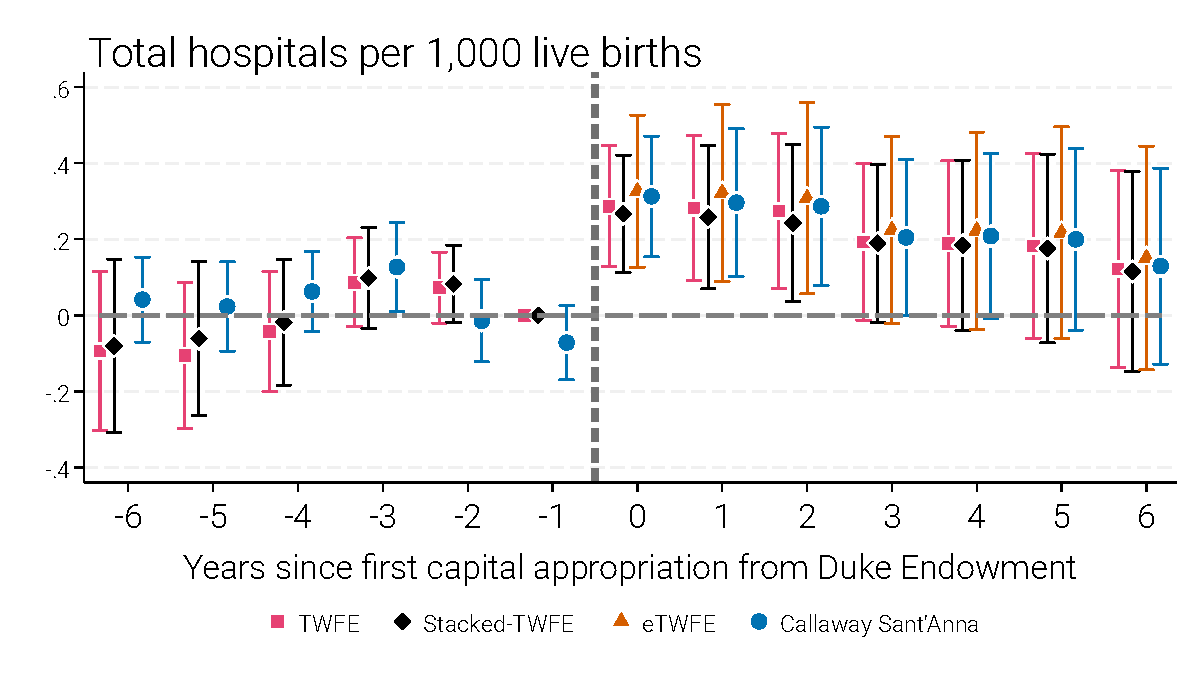
\includegraphics[width=\linewidth]{../analysis/output/appendix/figure_b1b1_total_hospitals_first_stage.pdf}  \end{subfigure}  
  \begin{subfigure}[b]{0.49\columnwidth}
    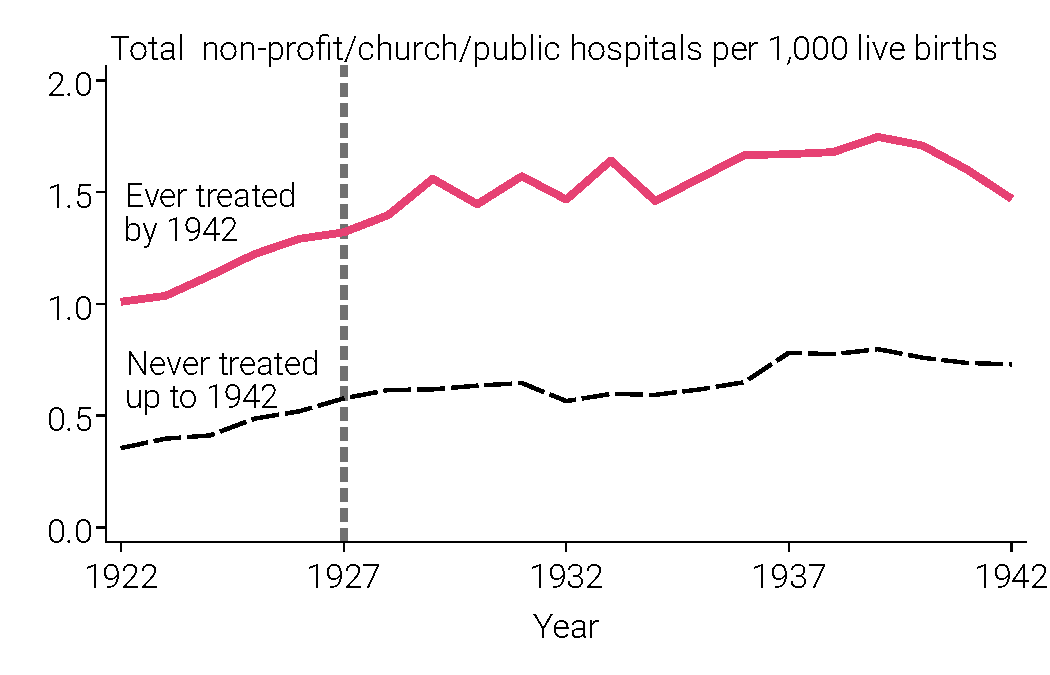
\includegraphics[width=\linewidth]{../analysis/output/appendix/figure_b1a2_likely_hospitals_by_year.pdf}  \end{subfigure}    
  \begin{subfigure}[b]{0.49\columnwidth}
    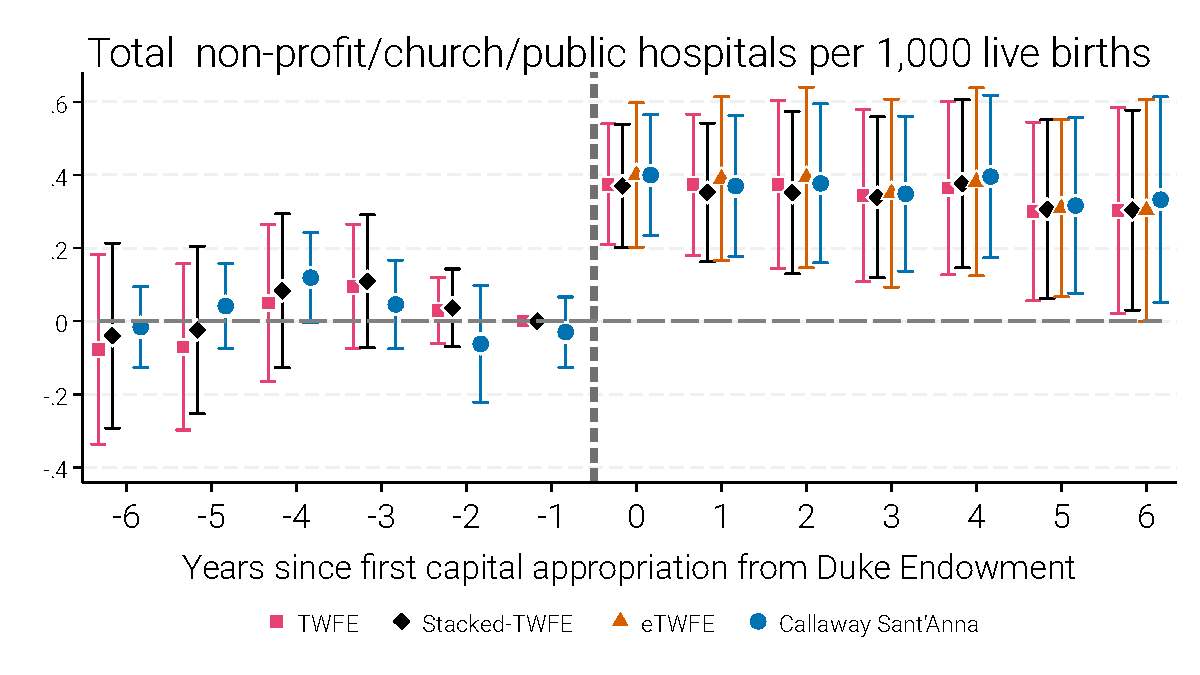
\includegraphics[width=\linewidth]{../analysis/output/appendix/figure_b1b2_likely_hospitals_first_stage.pdf}  \end{subfigure}  
  \begin{subfigure}[b]{0.49\columnwidth}
    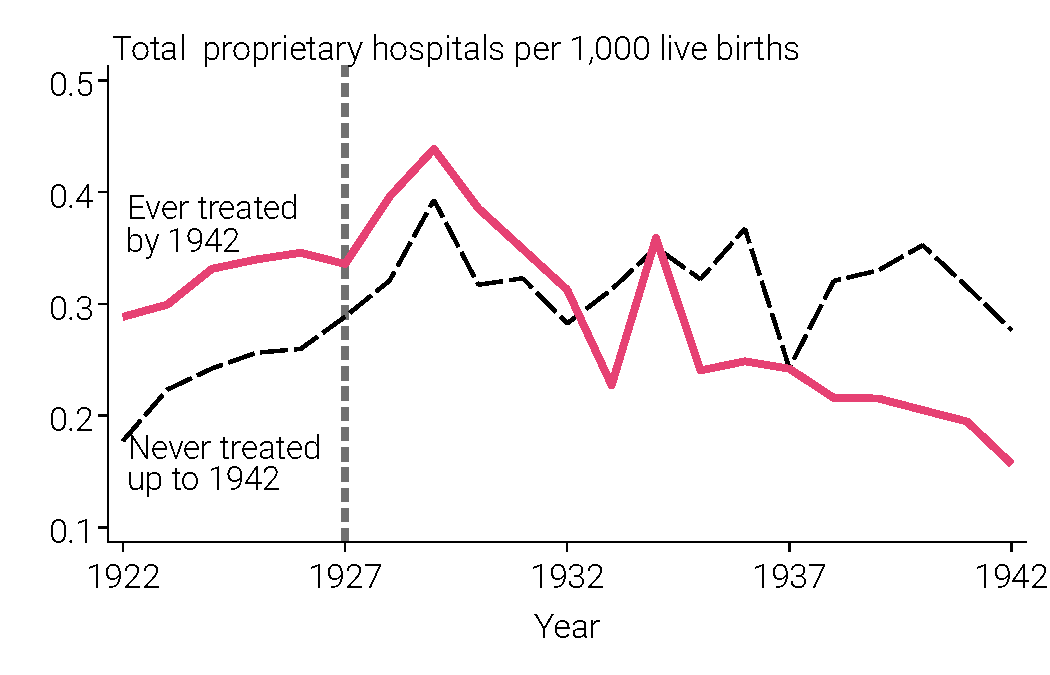
\includegraphics[width=\linewidth]{../analysis/output/appendix/figure_b1a3_private_hospitals_by_year.pdf}  \end{subfigure}
  \begin{subfigure}[b]{0.49\columnwidth}
    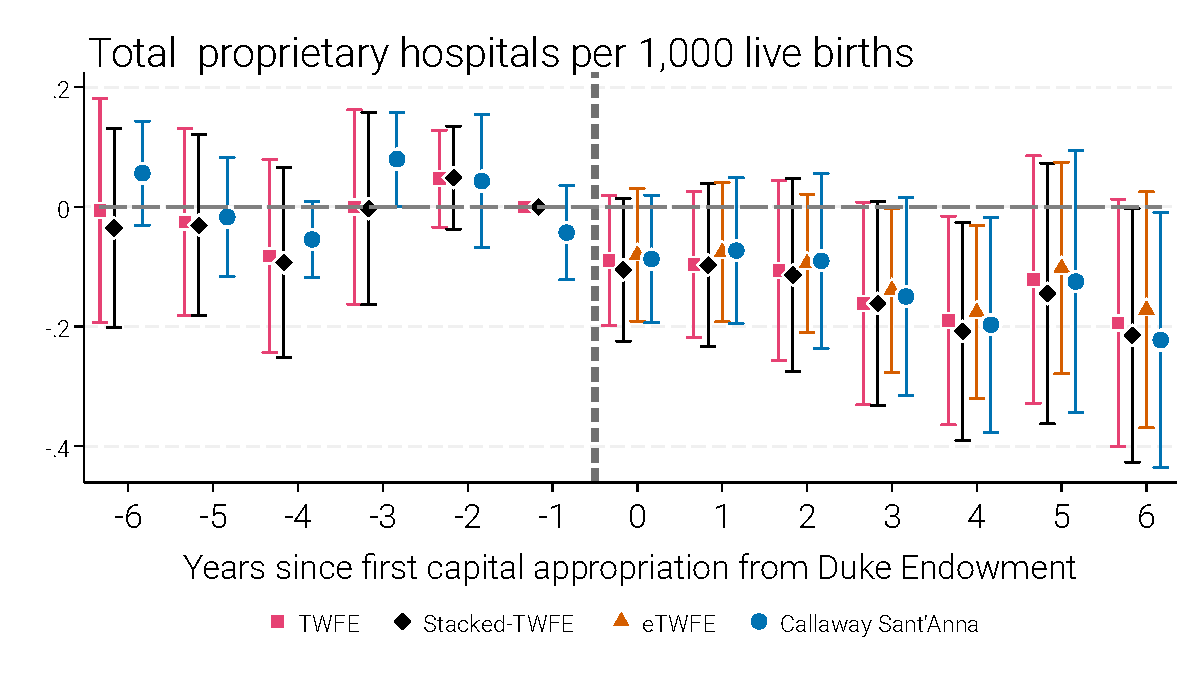
\includegraphics[width=\linewidth]{../analysis/output/appendix/figure_b1b3_private_hospitals_first_stage.pdf}  \end{subfigure}
  \end{minipage}
    \FnoteScript{
    \scriptsize{
        Column (a) plots plots shows the average annual number of hospitals in a county by Duke treatment status.
        Column (b) presents event-study estimates and 95\% confidence intervals for the lead and lag indicator variables for relative time periods from $t = -6$ to $t = 6$ around the first year that a county received an appropriation for capital expenditures from The Duke Endowment.
        More extreme relative time periods are estimated but not shown in the figures. 
        The omitted category is -1 year before initial treatment.
          An observational unit is a county by year cell.
          Each plot shows four event study estimators: two-way fixed effects, stacked regression,  extended two-way fixed effects \citepApp{Wooldridge2021}, and \citeApp{CS2021}.  
          All regressions include county and year fixed effects.
        Regressions are weighted by county-by-year of birth cohort size.
        Standard errors are clustered by county.
  The top row of plots shows the average annual number of general hospitals in a county by Duke treatment status.
  Appropriations for nurse homes are excluded from the definition of treatment. 
  Counties ``Ever treated by 1942'' first received an appropriation for Duke funding during the sample period, between 1927 and 1942, while counties ``Never treated up to 1942'' did not. 
  The middle row shows not-for-profits. 
  The final row shows proprietary hospitals. 
    }
    }
\end{figure}
\restoregeometry

%-------------------------------------------------------------------%
%                Appendix C - Doctors first stage - Alternate specs
%-------------------------------------------------------------------%

\FloatBarrier
\newpage
\newgeometry{top = 0.75in, bottom = 0.75in, right = 0.75in, left = 0.75in, footskip = 0.0in}
\section{First stage results for doctors and other health care professionals \label{sec:docs-first-stage-robust}}
\setcounter{table}{0}\renewcommand{\thetable}{\ref{sec:docs-first-stage-robust}\arabic{table}}
\setcounter{figure}{0}\renewcommand{\thefigure}{\ref{sec:docs-first-stage-robust}\arabic{figure}}

% Table C1
\begin{table}[!ht]\centering
    \centering
    \caption{Effects on number of doctors: Robustness to alternate estimators\label{tab:doctors-robust-alt-specs}}
    \begin{adjustbox}{width=.95\linewidth}
    \begin{threeparttable}
        \estauto{../analysis/output/appendix/table_c1_county_level_doctors_robustness.tex}{9}{S[table-format=2.4,table-column-width=20mm]}
        \Fignote{\pvaluenote 
            Each coefficient comes from a separate regression estimated by two-way fixed effects (columns 1 and 5), stacked regression (columns 2 and 6), extended two-way fixed effects  by \citeApp{Wooldridge2021} (columns 3 and 7), or \citeApp{CS2021} (columns 4 and 8).
            In columns 1 to 4, the dependent variable is the number of doctors (Panel A), the number of Black doctors (Panel B), or the number of White doctors (Panel C) in a county and publication year of the \emph{American Medical Directory} (AMD wave). 
            During the sample period, the AMD was published in 1921, 1923, 1925, 1927, 1929, 1931, 1934, 1936, 1938, 1940, and 1942. 
            Within each panel, the dependent variable is the number of doctors (top row); the number of high-quality doctors (middle row); or the number of low-quality doctors (bottom row). 
            A high-quality doctor is one who graduated from a medical school at least 4 years after it introduced a two-year college degree prerequisite for admission.
            All other doctors are considered low quality. 
            Columns 5 to 8 express the dependent variables as rates per 1,000 live births and follows the same structure as columns 1 to 4. 
            Each coefficient represents the change in the outcome variable due to receiving a capital appropriation from The Duke Endowment. 
            Control variables include \% illiterate, \% Black, \% other race, \% urban, retail sales per capita, and presence of a county health department.
            Weights are the average number of births in each county for the years in the AMD wave.
            Panels B and C drop counties that ever have zero race-specific births between 1922 and 1942 for any AMD wave. 
            Standard errors are clustered at the county level.
        }
    \end{threeparttable}
\end{adjustbox}
\end{table}
\restoregeometry

% Table C2
\newpage 
\newgeometry{top = 0.5in, bottom = 0.5in, right = 0.75in, left = 0.75in, footskip = 0.0in}
\begin{table}[ht]\centering
    \centering
    \caption{Effects on doctors: Robustness to other measures of high quality \label{tab:doctors-robust-alt-quality-high}}
    \begin{adjustbox}{width=0.9\linewidth}
    \begin{threeparttable}
        \estauto{../analysis/output/appendix/table_c2_county_level_doctors_alt_qual_high.tex}{2}{S[table-format=2.4,table-column-width=30mm]}
        \Fignote{\pvaluenote
            Each coefficient comes from a separate regression estimated by two-way fixed effects. 
            In column 1, the dependent variable is the number of doctors (Panel A), the number of Black doctors (Panel B), or the number of White doctors (Panel C) in a county and publication year of the \emph{American Medical Directory} (AMD wave). 
            During the sample period, the AMD was published in 1921, 1923, 1925, 1927, 1929, 1931, 1934, 1936, 1938, 1940, and 1942. 
            Column 2 expresses the dependent variables as rates per 1,000 live births and follows the same structure as column 1. 
            Within each panel, the dependent variable is a different measure of high-quality doctors: the number of doctors who graduated from a medical school at least 4 years after it introduced a two-year college degree prerequisite for admission, our main measure of high quality (top row); the number of doctors who graduated from a medical school with an A or A+ rating from the American Medical Association, (second row); the number of doctors who graduated from a medical school that existed and was approved in 1942 (third row); or the number of doctors who graduated from a medical school that did not close and was not absorbed by another school during the sample period (bottom row).             
            Each coefficient represents the change in the outcome variable due to receiving a capital appropriation from The Duke Endowment. 
            Control variables include \% illiterate, \% Black, \% other race, \% urban, retail sales per capita, and presence of a county health department.
            Weights are the average number of births in each county for the years in the AMD wave.
            Panels B and C drop counties that ever have zero race-specific births between 1922 and 1942 for any AMD wave. 
            Standard errors are clustered at the county level.
        }
    \end{threeparttable}
\end{adjustbox}
\end{table}
\restoregeometry

% Table C3
\newpage 
\newgeometry{top = 0.5in, bottom = 0.5in, right = 0.75in, left = 0.75in, footskip = 0.0in}
\begin{table}[ht]\centering
    \centering
    \caption{Effects on doctors: Robustness to other measures of low quality\label{tab:doctors-robust-alt-quality-low}}
    \begin{adjustbox}{width=.9\linewidth}
    \begin{threeparttable}
        \estauto{../analysis/output/appendix/table_c3_county_level_doctors_alt_qual_low.tex}{2}{S[table-format=2.4,table-column-width=30mm]}
        \Fignote{\pvaluenote
            Each coefficient comes from a separate regression estimated by two-way fixed effects. 
            In column 1, the dependent variable is the number of doctors (Panel A), the number of Black doctors (Panel B), or the number of White doctors (Panel C) in a county and publication year of the \emph{American Medical Directory} (AMD wave). 
            During the sample period, the AMD was published in 1921, 1923, 1925, 1927, 1929, 1931, 1934, 1936, 1938, 1940, and 1942. 
            Column 2 expresses the dependent variables as rates per 1,000 live births and follows the same structure as column 1. 
            Within each panel, the dependent variable is a different measure of low-quality doctors: the number of doctors who graduated from a medical school that did not introduce a two-year college degree prerequisite for admission at least 4 years prior to graduation, our main measure of low quality (top row); the number of doctors who graduated from a medical school without an A or A+ rating from the American Medical Association, (second row); the number of doctors who graduated from a medical school that did not exist or was not approved in 1942 (third row); or the number of doctors who graduated from a medical school that closed or was by another school during the sample period (bottom row). 
            Each coefficient represents the change in the outcome variable due to receiving a capital appropriation from The Duke Endowment. 
            Control variables include \% illiterate, \% Black, \% other race, \% urban, retail sales per capita, and presence of a county health department.
             Weights are the average number of births in each county for the years in the AMD wave.
            Panels B and C drop counties that ever have zero race-specific births between 1922 and 1942 for any AMD wave. 
            Standard errors are clustered at the county level.        
        }
    \end{threeparttable}
\end{adjustbox}
\end{table}
\restoregeometry

% Table C4
\begin{table}[ht]
    \centering
    \caption{Effects on doctors: Additional heterogeneity analyses\label{tab:doctors-more-het-quality}}
    \begin{adjustbox}{width=1.0\linewidth}
    \begin{threeparttable}
    \estauto{../analysis/output/appendix/table_c4_county_level_doctors_other_metrics.tex}{6}{S[table-format=2.4,table-column-width=20mm]}
    \Fignote{
        Each coefficient comes from a separate regression estimated by two-way fixed effects. 
        The unit of observation is a county and publication year of the \emph{American Medical Directory} (AMD wave). 
        During the sample period, the AMD was published in 1921, 1923, 1925, 1927, 1929, 1931, 1934, 1936, 1938, 1940, and 1942.
        Across the rows, the dependent variable is a measure of doctors belonging to a particular subset: surgeons, specialists, Fellows of the American Medical Association (AMA), AMA members, doctors who graduated from North Carolina medical schools, doctors under age 40, and doctors licensed after/before the publication of the Flexner Report in 1910. 
        In columns 1 to 3, the dependent variable is the number of doctors in the subset, while columns 4 to 6 expresses it as a rate per 1,000 live births. 
        Each coefficient represents the change in the outcome variable due to receiving a capital appropriation from The Duke Endowment. 
        Control variables include \% illiterate, \% Black, \% other race, \% urban, retail sales per capita, and presence of a county health department.
         Weights are the average number of births in each county for the years in the AMD wave.
        Standard errors are clustered at the county level. 
    }
    \end{threeparttable}
\end{adjustbox}
\end{table}

\newpage
\newgeometry{top = 0.5in, bottom = 0.5in, right = 0.5in, left = 0.5in, footskip = 0.0in}
\begin{figure}
    \caption[Black physician results by treatment status, quality, and event time.]{Black physician results by treatment status, quality, and event time.}
    \centering
  \begin{minipage}{\linewidth}
  \begin{subfigure}[b]{0.49\columnwidth}
    \caption{\scriptsize{Descriptive}}
    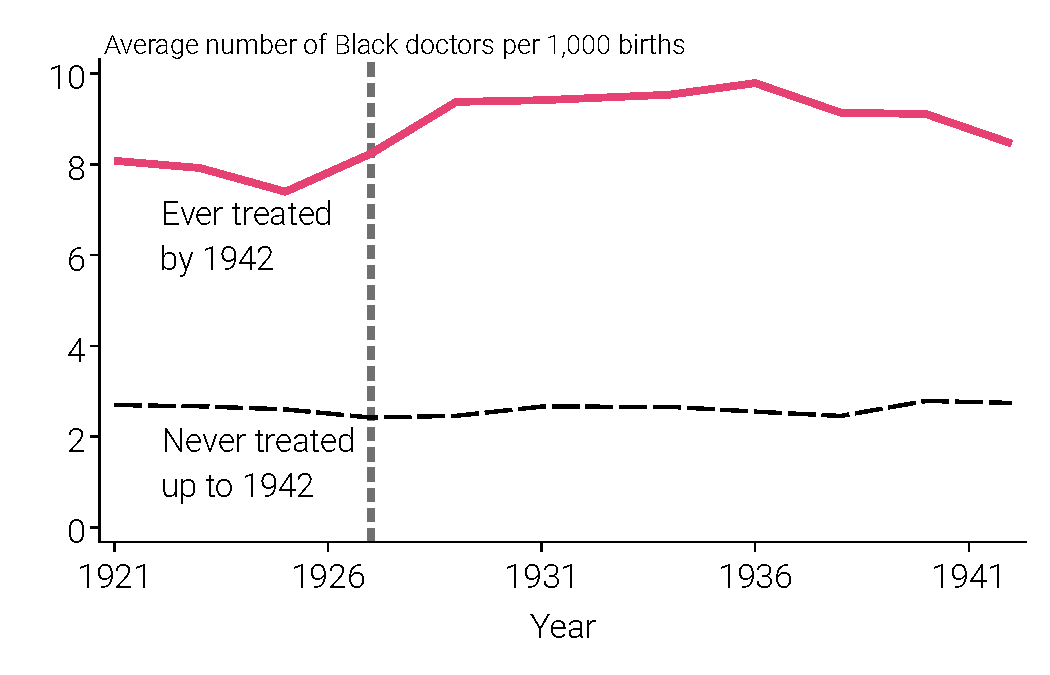
\includegraphics[width=.9\linewidth]{../analysis/output/appendix/figure_c1a1_black_rMD_by_treatment_status.pdf}
  \end{subfigure} 
  \begin{subfigure}[b]{0.49\columnwidth}
    \caption{\scriptsize{Event studies}}
    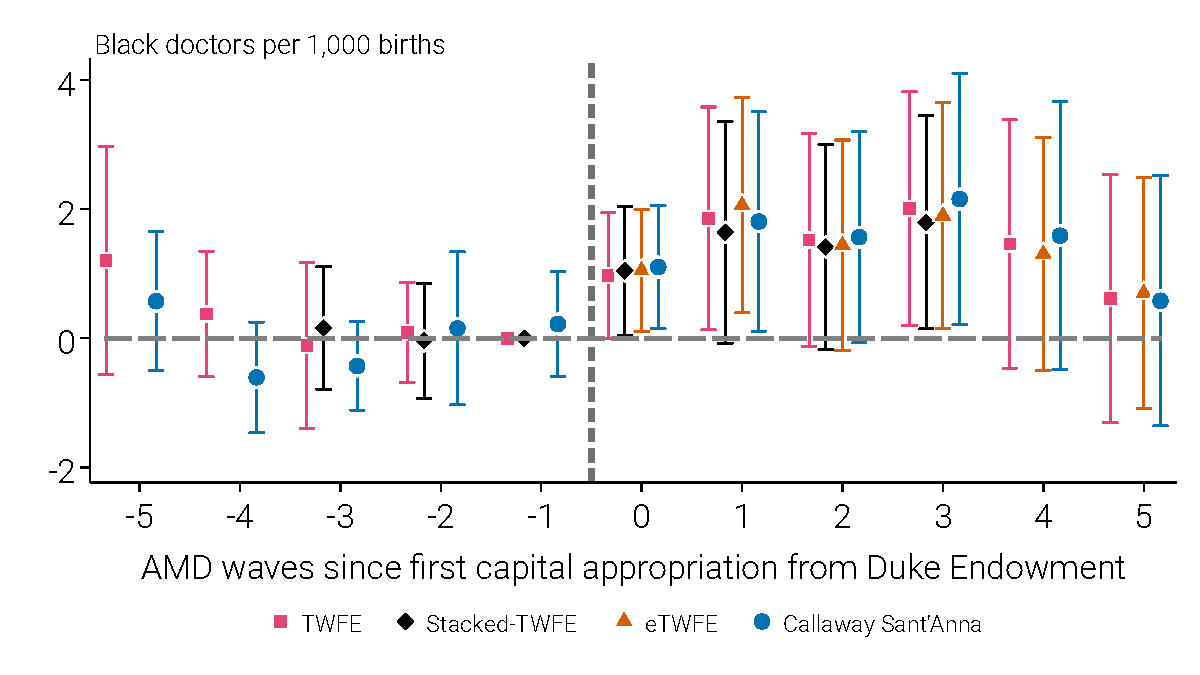
\includegraphics[width=\linewidth]{../analysis/output/appendix/figure_c1b1_all_black_doctors_first_stage.pdf}
  \end{subfigure}  
  \begin{subfigure}[b]{0.49\columnwidth}
    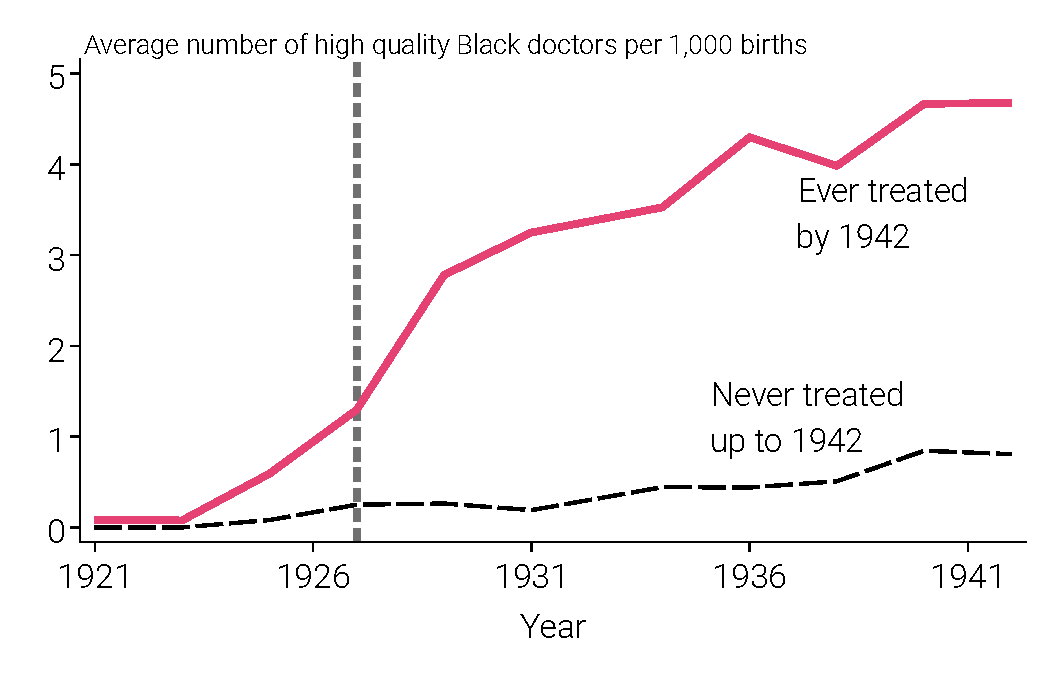
\includegraphics[width=.9\linewidth]{../analysis/output/appendix/figure_c1a2_black_rMD_good_by_treatment_status.pdf}
  \end{subfigure}    
  \begin{subfigure}[b]{0.49\columnwidth}
    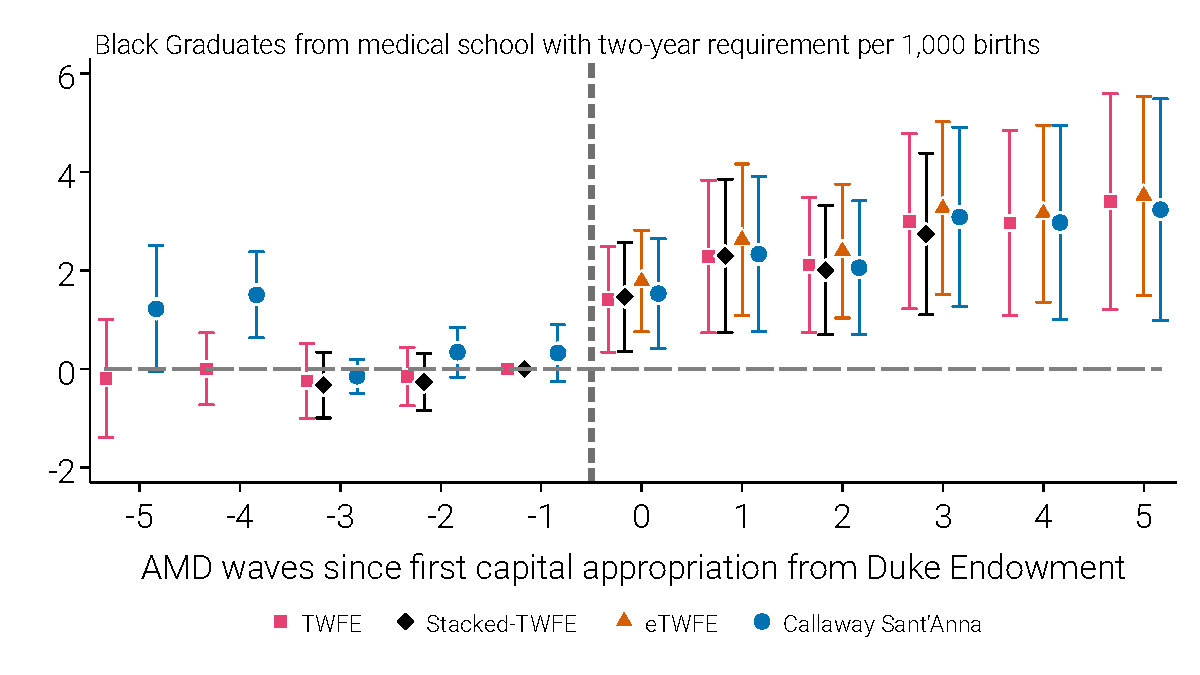
\includegraphics[width=\linewidth]{../analysis/output/appendix/figure_c1b2_good_black_doctors_first_stage.pdf}
  \end{subfigure}  
  \begin{subfigure}[b]{0.49\columnwidth}
    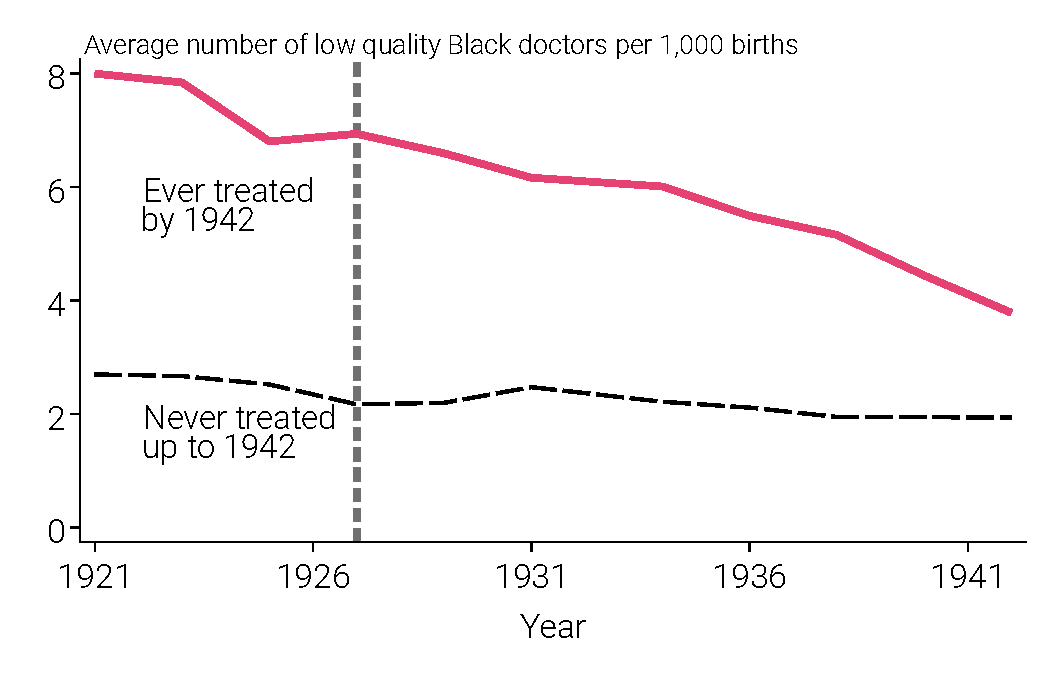
\includegraphics[width=.9\linewidth]{../analysis/output/appendix/figure_c1a3_black_rMD_bad_by_treatment_status.pdf}
  \end{subfigure}
  \begin{subfigure}[b]{0.49\columnwidth}
    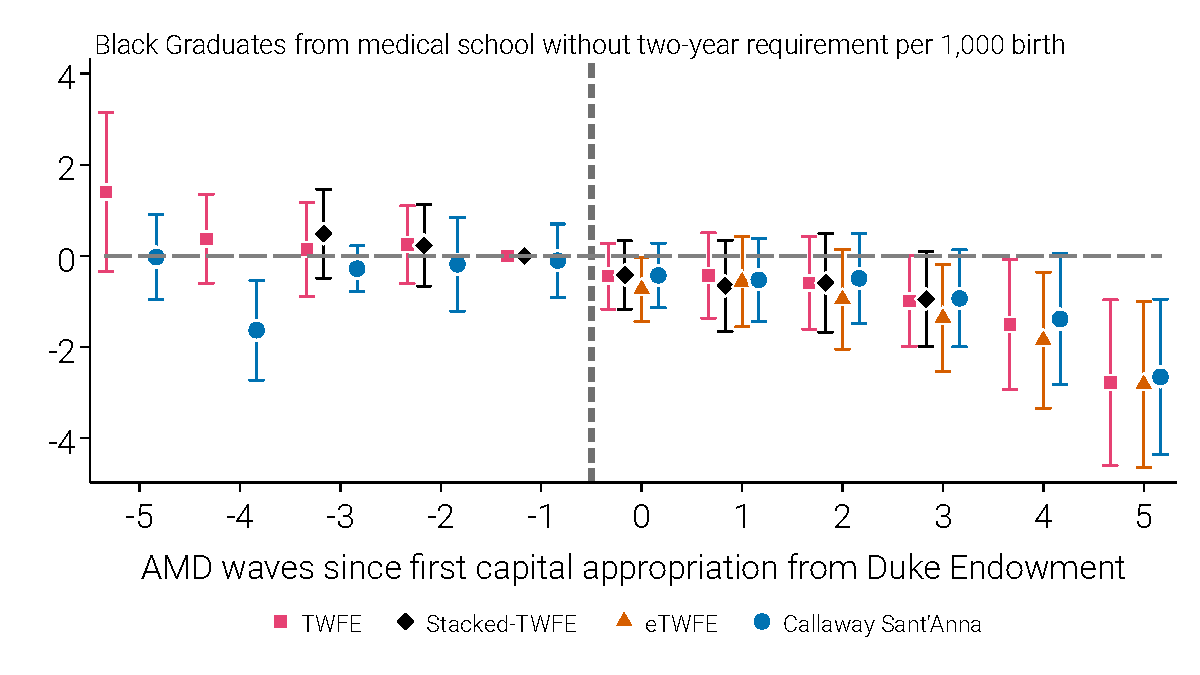
\includegraphics[width=\linewidth]{../analysis/output/appendix/figure_c1b3_bad_black_doctors_first_stage.pdf}
  \end{subfigure}
    \end{minipage}
    \FnoteScript{
    \scriptsize{
        Column (a) plots plots shows the average annual number of doctors in a county by Duke treatment status.
        Column (b) plots event study estimates of coefficient values and 95\% confidence intervals for the lead and lag indicator variables for relative time periods from $t=-5$ to $t = 5$ around the first AMD wave after a county received an appropriation for capital expenditures from The Duke Endowment (or from $t=-3$ to $t = 3$ in the case of the stacked event study).
        The first row presents the number of Black doctors per 1,000 births, the second rowplots the number of high-quality Black doctors per 1,000 births, and the last row plots the number of low-quality Black doctors per 1,000 births. 
        A high-quality doctor is one who graduated from a medical school at least 4 years after it introduced a two-year college degree prerequisite for admission.
        All other doctors are considered low quality. 
        Counties ``Ever treated by 1942'' first received Duke funding during the sample period, between 1927 and 1942, while counties ``Never treated up to 1942'' did not.
        Event time represents the number of \emph{American Medical Directory} (AMD) waves since the first year that a county received a capital appropriation from the Endowment.
        During the sample period, the AMD was published in 1921, 1923, 1925, 1927, 1929, 1931, 1934, 1936, 1938, 1940, and 1942. 
        More extreme relative time periods are estimated but not shown in the figures. 
	The omitted category is -1, the AMD wave before initial treatment.
        Each plot shows four event study estimators: two-way fixed effects, stacked regression,  extended two-way fixed effects \citepApp{Wooldridge2021}, and \citeApp{CS2021}.  
        An observational unit is a county-by-AMD wave.
        All regressions include county and AMD-wave fixed effects.
	Regressions are weighted by county of birth cohort size averaged over the two or three years of the AMD wave.
	Standard errors are clustered by county.
    }
    }
    \label{fig:black-md}
\end{figure}
\restoregeometry

\newpage
\newgeometry{top = 0.5in, bottom = 0.5in, right = 0.5in, left = 0.5in, footskip = 0.0in}
\begin{figure}
    \caption[White physician results by treatment status, quality, and event time.]{White physician results by treatment status, quality, and event time.}
    \centering
  \begin{minipage}{\linewidth}
  \begin{subfigure}[b]{0.49\columnwidth}
    \caption{\scriptsize{Descriptive}}
    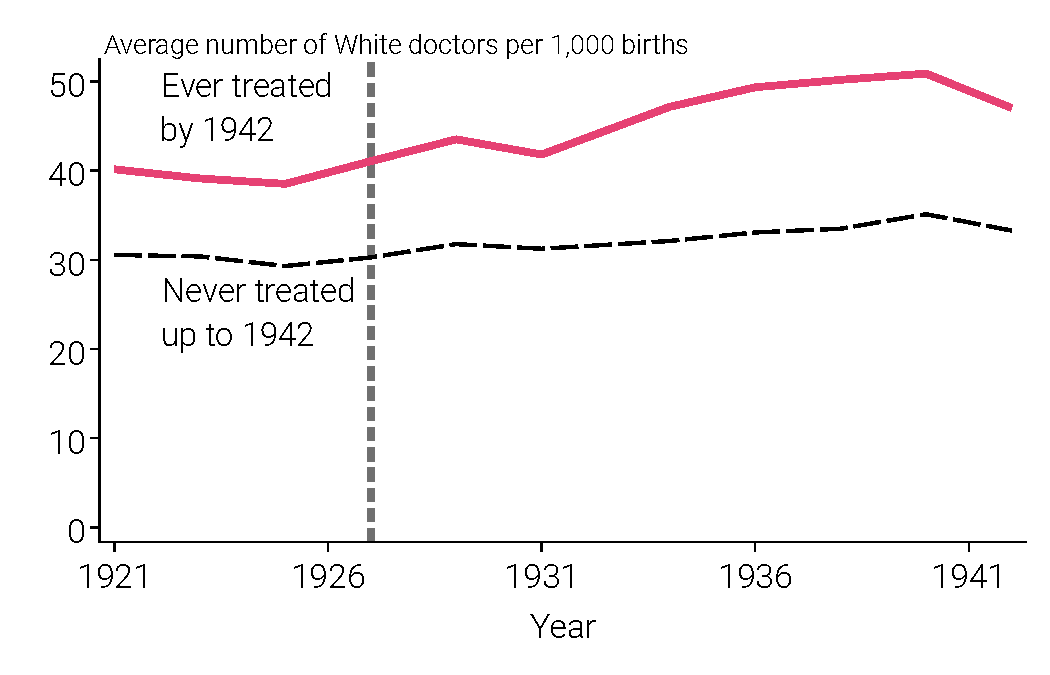
\includegraphics[width=.9\linewidth]{../analysis/output/appendix/figure_c2a1_white_rMD_by_treatment_status.pdf}
  \end{subfigure} 
  \begin{subfigure}[b]{0.49\columnwidth}
    \caption{\scriptsize{Event studies}}
    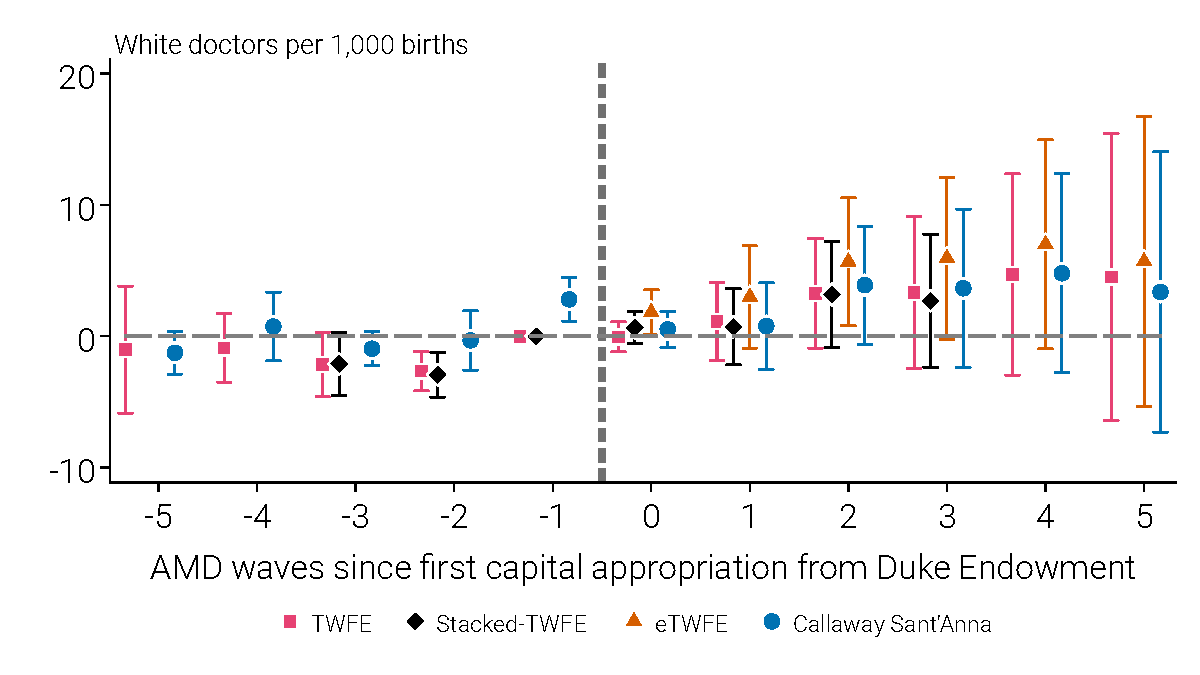
\includegraphics[width=\linewidth]{../analysis/output/appendix/figure_c2b1_all_white_doctors_first_stage.pdf}
  \end{subfigure}  
  \begin{subfigure}[b]{0.49\columnwidth}
    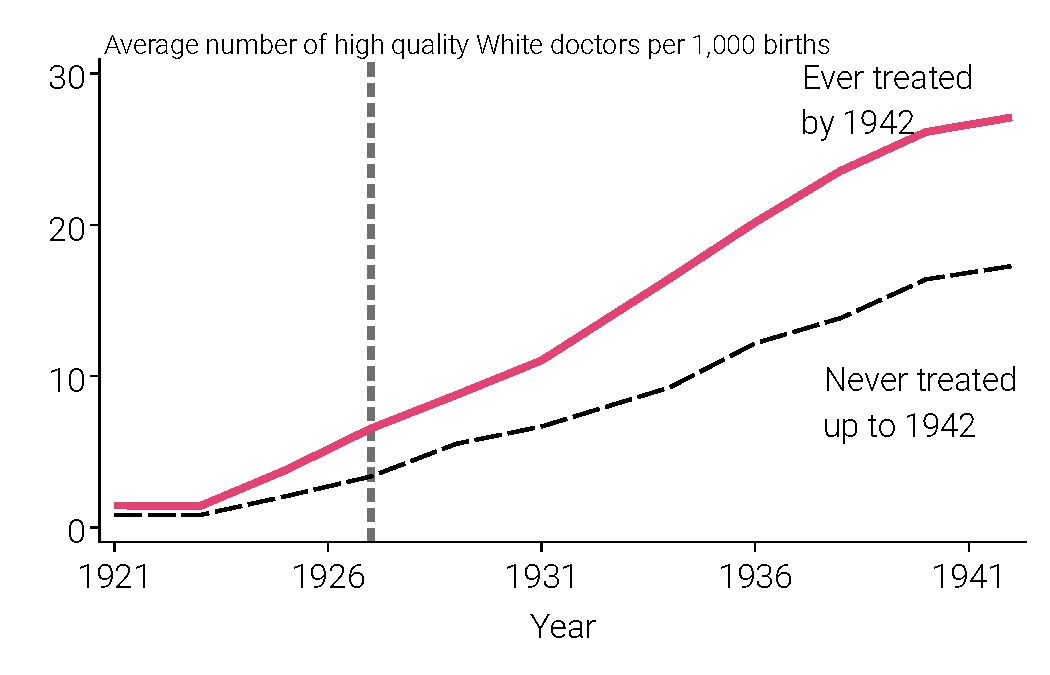
\includegraphics[width=.9\linewidth]{../analysis/output/appendix/figure_c2a2_white_rMD_good_by_treatment_status.pdf}
  \end{subfigure}    
  \begin{subfigure}[b]{0.49\columnwidth}
    \includegraphics[width=\linewidth]{../analysis/output/appendix/figure_c2b2_good_white_doctors_first_stage.pdf}
  \end{subfigure}  
  \begin{subfigure}[b]{0.49\columnwidth}
    \includegraphics[width=.9\linewidth]{../analysis/output/appendix/figure_c2a3_white_rMD_bad_by_treatment_status.pdf}
  \end{subfigure}
  \begin{subfigure}[b]{0.49\columnwidth}
    \includegraphics[width=\linewidth]{../analysis/output/appendix/figure_c2b3_bad_white_doctors_first_stage.pdf}
  \end{subfigure}
  \end{minipage}
    \FnoteScript{
    \scriptsize{
        Column (a) plots plots shows the average annual number of doctors in a county by Duke treatment status.
        Column (b) plots event study estimates of coefficient values and 95\% confidence intervals for the lead and lag indicator variables for relative time periods from $t=-5$ to $t = 5$ around the first AMD wave after a county received an appropriation for capital expenditures from The Duke Endowment (or from $t=-3$ to $t = 3$ in the case of the stacked event study).
        The first row presents the number of White doctors per 1,000 births, the second rowplots the number of high-quality White doctors per 1,000 births, and the last row plots the number of low-quality White doctors per 1,000 births. 
        A high-quality doctor is one who graduated from a medical school at least 4 years after it introduced a two-year college degree prerequisite for admission.
        All other doctors are considered low quality. 
        Counties ``Ever treated by 1942'' first received Duke funding during the sample period, between 1927 and 1942, while counties ``Never treated up to 1942'' did not.
        Event time represents the number of \emph{American Medical Directory} (AMD) waves since the first year that a county received a capital appropriation from the Endowment.
        During the sample period, the AMD was published in 1921, 1923, 1925, 1927, 1929, 1931, 1934, 1936, 1938, 1940, and 1942. 
        More extreme relative time periods are estimated but not shown in the figures. 
	The omitted category is -1, the AMD wave before initial treatment.
        Each plot shows four event study estimators: two-way fixed effects, stacked regression,  extended two-way fixed effects \citepApp{Wooldridge2021}, and \citeApp{CS2021}.  
        An observational unit is a county-by-AMD wave.
        All regressions include county and AMD-wave fixed effects.
	Regressions are weighted by county of birth cohort size averaged over the two or three years of the AMD wave.
	Standard errors are clustered by county.
    }
    }
    \label{fig:white-md}
\end{figure}
\restoregeometry

\begin{figure}[!ht]
  \caption{Employment of other health care professionals}
  \begin{minipage}{\linewidth}
  \begin{subfigure}[b]{0.49\columnwidth}
    \caption{\scriptsize{Descriptive}}
    \includegraphics[width=.9\linewidth]{../analysis/output/appendix/figure_c3a1_med_profs_by_treatment_status_nurse.pdf}
  \end{subfigure} 
  \begin{subfigure}[b]{0.49\columnwidth}
    \caption{\scriptsize{Event studies}}
    \includegraphics[width=\linewidth]{../analysis/output/appendix/figure_c3b1_event_study_hosp_staff_nurse.pdf}
    \end{subfigure}  
  \begin{subfigure}[b]{0.49\columnwidth}
    \includegraphics[width=.9\linewidth]{../analysis/output/appendix/figure_c3a2_med_profs_by_treatment_status_hosp_attendant.pdf}
  \end{subfigure}    
  \begin{subfigure}[b]{0.49\columnwidth}
    \includegraphics[width=\linewidth]{../analysis/output/appendix/figure_c3b2_event_study_hosp_staff_hosp_attendant.pdf}
    \end{subfigure}  
  \begin{subfigure}[b]{0.49\columnwidth}
    \includegraphics[width=.9\linewidth]{../analysis/output/appendix/figure_c3a3_med_profs_by_treatment_status_hosp_clerical.pdf}
  \end{subfigure}
  \begin{subfigure}[b]{0.49\columnwidth}
    \includegraphics[width=\linewidth]{../analysis/output/appendix/figure_c3b3_event_study_hosp_staff_hosp_clerical.pdf}
  \end{subfigure}
  \end{minipage}
  \Fnote{
        The figures in column (a) plot the average number of nurses (top row), as well as attendants (middle row) and clerical workers (bottom row) employed in the medical industry in 1920, 1930, and 1940, separately for North Carolina counties that were treated by Duke support by 1940 and those that were not.
        Column (b) displays event studies for the same set of outcomes, in which each unit of event time is a decade (the time between census waves). 
        Event studies are estimated by two-way fixed effects or \citeApp{CS2021}. 
        Data on the number of nurses and medical professionals come from aggregating individual records in the complete count censuses \citepApp{IPUMSUSA2023}. 
    }
  \label{fig:hosp-staff}
\end{figure}

%-------------------------------------------------------------------%
%                Appendix D - Infant mortality: Additional results
%-------------------------------------------------------------------%

\FloatBarrier
\newpage
\newgeometry{top = 0.75in, bottom = 0.75in, right = 0.75in, left = 0.75in, footskip = 0.0in}
\begin{landscape}
\section{Infant mortality: Additional results\label{sec:infant-mortality-robust}}
\setcounter{table}{0}\renewcommand{\thetable}{\ref{sec:infant-mortality-robust}\arabic{table}}

% Table D1
\begin{table}[!ht]\centering
    \centering
    \caption{Robustness of infant mortality results to alternate estimators\label{tab:infant-mortality-alt-specs}}
    \begin{adjustbox}{width=.9\linewidth}
    \begin{threeparttable}
        \estauto{../analysis/output/appendix/table_d1_infant_mortality_robustness.tex}{9}{S[table-format=2.4,table-column-width=20mm]}
        \Fignote{\pvaluenote 
            Each coefficient comes from a separate regression estimated by Poisson (columns 1 and 5), stacked Poisson with a balanced panel (columns 2 and 6), the extended two-way fixed effects estimator by \citeApp{Wooldridge2021} (columns 3 and 7), or the \citeApp{CS2021} estimator (columns 4 and 8).
            In columns 1 to 4, the dependent variable is the number of infant deaths (Panel A), the number of Black infant deaths (Panel B), or the number of White infant deaths (Panel C) in a county-by-year of birth cohort. 
            Columns 5 to 8 express the dependent variables as rates per 1,000 live births and follow the same structure as columns 1 to 4. 
            Each coefficient represents the percent change in the outcome variable due to receiving a capital appropriation from The Duke Endowment. 
            Coefficients are transformed in the following way: $100\times (exp(\beta) - 1)$. Standard errors are calculated using the delta method. 
            The weights are the number of births in a county and year.
            Panels B and C drop counties that ever have zero race-specific births between 1922 and 1942.
            Standard errors are clustered at the county level.
        }
    \end{threeparttable}
\end{adjustbox}
\end{table}
\end{landscape}

% Table D2
\setcounter{table}{1}\renewcommand{\thetable}{\ref{sec:infant-mortality-robust}\arabic{table}}
\begin{table}[!ht]\centering
    \centering
    \caption{Robustness of infant mortality results to log specification\label{tab:infant-mortality-log-specs}}
    \begin{adjustbox}{width=0.9\linewidth}
    \begin{threeparttable}
        \estauto{../analysis/output/appendix/table_d2_infant_mortality_log_specs.tex}{9}{S[table-format=2.4,table-column-width=20mm]}
        \Fignote{\pvaluenote 
            Each coefficient comes from a separate regression estimated by two-way fixed effects (column 1), stacked two-way fixed effects (column 2), the extended two-way fixed effects estimator by \citeApp{Wooldridge2021} (column 3), or the \citeApp{CS2021} estimator (column 4). 
            The dependent variable is the natural log of infant mortality rate per 1,000 live births (Panel A), the natural log of Black infant mortality rate per 1,000 live births (Panel B), or the natural log White infant mortality rate per 1,000 live births (Panel C) in a county-by-year of birth cohort. 
            Each coefficient represents the change in the outcome variable due to receiving a capital appropriation from The Duke Endowment. 
            The weights are the number of births in a county and year.
            Panels B and C drop observations with zero race-specific births or infant deaths while the log transformation drops county-year observations with zero deaths.
            Standard errors are clustered at the county level.
        }
    \end{threeparttable}
\end{adjustbox}
\end{table}

% Figure D1
\setcounter{figure}{0}\renewcommand{\thefigure}{\ref{sec:infant-mortality-robust}\arabic{figure}}
\begin{figure}[ht]
  \caption{Stacked Poisson event studies for effects of Duke support on pooled infant mortality rate}
  \begin{minipage}{\linewidth}
  \begin{subfigure}[b]{0.49\columnwidth}
    \caption{\scriptsize{Without controls}}
    \includegraphics[width=\linewidth]{../analysis/output/appendix/figure_d1a_event_study_pooled_imr_stacked_poisson_kappa_3_controls_no.pdf}
    \includegraphics[width=\linewidth]{../analysis/output/appendix/figure_d1a_event_study_pooled_imr_stacked_poisson_kappa_4_controls_no.pdf}
    \includegraphics[width=\linewidth]{../analysis/output/appendix/figure_d1a_event_study_pooled_imr_stacked_poisson_kappa_5_controls_no.pdf}
    \includegraphics[width=\linewidth]{../analysis/output/appendix/figure_d1a_event_study_pooled_imr_stacked_poisson_kappa_6_controls_no.pdf}
  \end{subfigure}
  \hfill %%
  \begin{subfigure}[b]{0.49\columnwidth}
    \caption{\scriptsize{With controls}}
    \includegraphics[width=\linewidth]{../analysis/output/appendix/figure_d1b_event_study_pooled_imr_stacked_poisson_kappa_3_controls_yes.pdf}
    \includegraphics[width=\linewidth]{../analysis/output/appendix/figure_d1b_event_study_pooled_imr_stacked_poisson_kappa_4_controls_yes.pdf}
    \includegraphics[width=\linewidth]{../analysis/output/appendix/figure_d1b_event_study_pooled_imr_stacked_poisson_kappa_5_controls_yes.pdf}
    \includegraphics[width=\linewidth]{../analysis/output/appendix/figure_d1b_event_study_pooled_imr_stacked_poisson_kappa_6_controls_yes.pdf}
  \end{subfigure}
  \end{minipage}
  \FnoteScript{
  \scriptsize{
    Extensive margin intent-to-treat estimates.
    Each figure presents event studies from a separate stacked regression including county and year fixed effects.
    The dependent variable is the pooled infant mortality rate per 1,000 live births.
    Each stack includes treated counties from a single treatment timing group and control counties that are not treated within the event time window of $\pm\kappa$. Across the rows of the figure, $\kappa$ varies from 3 to 6 leads and lags.
    All samples include 11 stacks. We exclude the 1940 timing groups since forming a complete stack for this group would require using data outside our main sample period from 1922 to 1942.
    Control variables in column (b) include \% illiterate, \% Black, \% other race, \% urban, retail sales per capita, and presence of a county health department. Standard errors are estimated using the delta method and are clustered at the county level. The shaded areas are 95\% confidence intervals based on these standard errors. 
    }
    }
  \label{fig:stacked-poisson-event-studies}
\end{figure}
\restoregeometry

%-------------------------------------------------------------------%
%      Appendix E - Duke funding: Heterogeneity by project type
%-------------------------------------------------------------------%

\FloatBarrier
\newpage
\newgeometry{top = 0.75in, bottom = 0.75in, right = 1.0in, left = 1.0in, footskip = 0.0in}
\section{Duke funding: Heterogeneity by project type \label{sec:het-proj-type}}
\setcounter{table}{0}\renewcommand{\thetable}{\ref{sec:het-proj-type}\arabic{table}}
\setcounter{figure}{0}\renewcommand{\thefigure}{\ref{sec:het-proj-type}\arabic{figure}}

% Table E1
\begin{table}[!ht]\centering
  \begin{adjustbox}{width=0.7\textwidth}
  \centering
    \begin{threeparttable}
        \caption{Appropriation and payment details by project type\label{tab:app-payment-summary}}
        \estauto{../analysis/output/appendix/table_e1_het_summary.tex}{5}{S[table-format=1.2,table-column-width=15mm, table-alignment = center]}
        \Fignote{
            Summary statistics for appropriations and payments from The Duke Endowment in millions of 2017 dollars.
            The sample includes all appropriations for hospitals in North Carolina initiated between 1927 and 1942 and all payments made on these appropriations up to and including 1962, 
            The unit of observation is a unique appropriation identifier. 
            An appropriation identifier links all appropriations and payments made on those appropriations starting from the initial appropriation for a hospital until all active appropriations have been paid off. 
            Any subsequent appropriations for a given hospital are assigned a separate appropriation identifier. 
            Some appropriations or payments may apply to more than one project type.
        }
    \end{threeparttable}
   \end{adjustbox}
\end{table}

% Figure E1
\begin{figure}[!ht]
    \caption[Appropriation to payment]{Time from appropriation to payment}
    \centering
    \begin{subfigure}{.7\textwidth}
        \centering
        \includegraphics[width=\linewidth]{../analysis/output/appendix/figure_e1_share_rec_pay_by_years_since_app.pdf}
    \end{subfigure}
    \Fnote{This figure plots the share of unique appropriations by the number of years after the initial appropriation when the first payment was received by the hospital.}
    \label{fig:appropriation-to-payment}
\end{figure}
\restoregeometry

% Figure E2
\newpage
\newgeometry{top = 0.5in, bottom = 0.5in, right = 0.5in, left = 0.5in, footskip = 0.0in}
\begin{figure}[!ht]
    \caption{Differential effects of Duke support by project type: Extensive and intensive margin estimates}
    \centering
    \begin{subfigure}{.59\textwidth}
        \centering
        \caption{Intent to treat (binary)}
        \includegraphics[width=\linewidth]{../analysis/output/appendix/figure_e2a_bin_pooled.pdf}
    \end{subfigure}
    \begin{subfigure}{.59\textwidth}
        \centering
        \caption{Appropriation amount (Effect of 1 \$ million)}
        \includegraphics[width=\linewidth]{../analysis/output/appendix/figure_e2b_app_pooled.pdf}
    \end{subfigure}
    \begin{subfigure}{.59\textwidth}
        \centering
        \caption{Payment amount (Effect of 1 \$ million)}
        \includegraphics[width=\linewidth]{../analysis/output/appendix/figure_e2c_pay_pooled.pdf}
    \end{subfigure}
    \Fnote{
		Each point estimate comes from a separate regression and represents the percent reduction in infant mortality due to Duke support.
		Treatment is defined as category-specific support. 
        Each category-specific sample drops counties that only received funding for other project categories. 
		Panel A reports an intent to treat analysis with a binary treatment of having received a capital appropriation.
		A coefficient of -10 would mean that infant mortality declines by 10\%.
        Coefficients reported in the figure are transformed in the following way: $100\times (exp(\beta) - 1)$.
        In panel B, treatment is defined as appropriations to the county while in panel C it is defined as actual payments. 
        Monetary amounts are converted to millions of 2017 dollars.
		All regressions include county and year fixed effects.
		Control variables include \% illiterate, \% Black, \% other race, \% urban, retail sales per capita, and presence of a county health department.
		The weights are the number of births in a county and year.
		Standard errors are estimated using the delta method and are clustered at the county-level.
	}
    \label{fig:het-effects-by-project-type}
\end{figure}
\restoregeometry


%-------------------------------------------------------------------%
%                Appendix F - Later-life mortality
%-------------------------------------------------------------------%

\FloatBarrier
\newpage
\section{Long-run analysis: Additional details, robustness checks, and event studies\label{sec:later-life-mortality-robust}}
\setcounter{table}{0}\renewcommand{\thetable}{\ref{sec:later-life-mortality-robust}\arabic{table}}
\setcounter{figure}{0}\renewcommand{\thefigure}{\ref{sec:later-life-mortality-robust}\arabic{figure}}

% Event-studies
\subsection{Event studies\label{sec:later-life-mortality-es}}
\singlespacing

Before reviewing event study results for long-run mortality, it is helpful to recall that our long-run analysis estimates the effect of the \emph{same} treatment as the short-run analysis -- Duke support \emph{around the time of birth}. 
In all event studies, event time is defined as the year of birth minus the year of first capital appropriation from The Duke Endowment. 
For example, for a county that received its first capital appropriation in 1935, the 1940 birth cohort would receive an event-time value of 5. 
Thus a positive event time indicates that treatment occurred in the year of birth \emph{or before}. 
Likewise, -5 in event time value represents a cohort born in a county that received its first capital appropriation five years after the birth year (i.e., when the cohort was five years old).


We report three event study specifications: one that is directly comparable to the short-run analyses (examining the effect in event time in the six years before and after treatment); one that extends the time before birth during which a county could have received support to ten years; and another that prevents compositional changes in the treated counties from muddying the interpretation of the event study estimates. 
We discuss each of these event studies in turn below. 

First, in Figure~\ref{fig:lr-event-study}, we consider event study estimates that are directly comparable to the event studies for the short-run analyses. 
We follow \citetApp{goodman-baconLongRunEffectsChildhood2021} by making our reference age far from the year of birth so that we can better understand if there are dynamic treatment effects at other points in childhood. 
We opt for $-$6 to be our reference year because we have far fewer years of treated observations contributing to these event study analyses than in \citetApp{goodman-baconLongRunEffectsChildhood2021}, as displayed in Figure~\ref{fig:lr-unbalanced-event-time}. 
Thus, event-time coefficient $k < 0$ can be interpreted as the effect of first receiving a capital appropriation at age $k$ relative to the effect of receipt at age six, while event-time coefficient $k \geq 0$ can be interpreted as the effect of receiving a capital appropriation around birth relative to the effect of receipt at age six. 

Figure~\ref{fig:lr-event-study} shows a somewhat noisy, but clear pattern, demonstrating that long-run mortality is lower for those who had a capital appropriation in the first year of their life (event time of -1) or earlier (positive event time). 
The fact that there are no trends in the \emph{positive} event-time coefficients is comforting to us as this indicates that there were no trends differentially affecting those county-birth-year cohorts that received an appropriations before their year of birth. For example, medical technology could have been consistently improving in treated counties, thus gradually improving life expectancy at birth for each birth-year cohort. If this were the case, then we would expect to find larger long-run mortality reductions for cohorts born ten years after an appropriation than for cohorts born three years after an appropriation. 



In Figure~\ref{fig:lr-event-study-extend}, we consider a second event study that extends the analysis to include cohorts born in a county up to 10 years after the first capital appropriation received by the county. 
This extension introduces minimal additional imbalance since there are a large number of treated birth cohorts contributing to identify these event time estimates. 
This extended analysis solidifies the result from the event study in Figure~\ref{fig:lr-event-study} by showing clearly that long-run mortality is lower -- and not trending differentially -- for those who were born in counties that had received a capital appropriation before or during the year of birth. 


While these event studies largely confirm our overall findings, we find them potentially challenging to interpret due to the imbalance in observations across event times displayed in Figure~\ref{fig:lr-unbalanced-event-time}. 
Some of the noise, or possibly some of the effect, could be driven by differences across event times in the set of counties contributing to the estimation of each coefficient. 
Thus, in Figure~\ref{fig:lr-event-study-balance}, we consider a final event study that restricts the set of treated counties to those that are observable from event times -2 to +6 and find clear evidence of a differential effect of Duke support on long-run mortality around the time of birth. 


% Table F1
\newgeometry{top = 0.75in, bottom = 0.75in, right = 0.75in, left = 0.75in, footskip = 0.0in}
\begin{landscape}
\begin{table}[ht]\centering
  \begin{adjustbox}{width=0.8\textwidth}
  \centering
    \begin{threeparttable}
      \caption{Effect of Duke support around time of long-run birth on mortality at ages 56 to 64, adding death rates to main table}
     \estauto{../analysis/output/appendix/table_F1_later_life_mortality_with_rates.tex}{6}{S[table-format=2.2,table-column-width=20mm, table-alignment = center]}
      \label{tab:llmr-did-poisson-add-rates}
      \Fignote{\pvaluenote
            Each coefficient comes from a separate Poisson pseudo maximum likelihood regression.
            The unit of observation is a birth county by birth year by follow-up age triplet.
            Birth cohorts are restricted to 1932 to 1941.
            Deaths are restricted to ages 56 to 64 and years 1988 to 2005.
            In columns 1 to 3, the dependent variable is the number of age-specific deaths.
            In columns 4 to 6, it is the death rate per 1,000 population in a county-by-year of birth cohort \citepMain{SEER2022}.
            Each coefficient represents the percent reduction in later-life mortality due to receiving a capital appropriation from The Duke Endowment around the time of birth.
            A coefficient of -10 would mean that later-life mortality declines by 10\%.
            Coefficients reported in the table are transformed in the following way: $100\times (exp(\beta) - 1)$.
            Control variables in columns 3 and 6 include flexible interactions of age fixed effects with \% illiterate, \% Black, \% other race, \% urban, retail sales per capita, and presence of a county health department.
            In columns 2 to 3 and 5 to 6, the weights are county-by-year birth cohort size.
            Panels B and C drop counties that include cohorts with zero births in any year between 1932 and 1941. 
            Observations differ across the two samples as observations that are perfectly separated by either county-of-birth by follow-up age fixed effects or year-of-birth by follow-up age fixed effects are dropped. 
            The bottom row presents a p-value from the interaction of race with our treatment variable from a model that fully interacts all variables with race. 
            All specifications include county-of-birth fixed effects interacted with follow-up age fixed effects and year-of-birth fixed effects interacted with follow-up age fixed effects. 
		  Standard errors are estimated using the delta method and are clustered at the county level.
        }
    \end{threeparttable}
   \end{adjustbox}
\end{table}
\end{landscape}
\restoregeometry


% Table F2
\begin{table}[!ht]\centering
  \begin{adjustbox}{width=0.75\textwidth}
  \centering
    \begin{threeparttable}
      \caption{Long-run mortality robustness: Cumulative mortality by county and year of birth\label{tab:llmr-did-poisson-robust-cumulative}}
     \estauto{../analysis/output/appendix/table_F2_later_life_mortality_collapsed.tex}{3}{S[table-format=2.2,table-column-width=20mm, table-alignment = center]}
      \Fignote{\pvaluenote
            Each coefficient comes from a separate Poisson pseudo maximum likelihood regression.
            The unit of observation is a birth county by birth year.
            Birth cohorts are restricted to 1932 to 1941.
            Deaths are restricted to ages 56 to 64 and years 1988 to 2005.
            The dependent variable is the cumulative number of deaths.
            The coefficient \emph{Treated} represents the percent reduction in long-run mortality at ages 56 to 64 due to receiving a capital appropriation from The Duke Endowment around the time of birth.
            A coefficient of -10 would mean that long-run mortality declines by 10\%.
            Coefficients reported in the table are transformed in the following way: $100\times (exp(\beta) - 1)$.
            Control variables in column 3 include flexible interactions of age fixed effects with \% illiterate, \% Black, \% other race, \% urban, retail sales per capita, and presence of a county health department.
            In columns 2 to 3, the weights are county-by-year birth cohort size.
            Panels B and C drop counties that include cohorts with zero births in any year between 1932 and 1941.
            All specifications include county-of-birth fixed effects interacted with follow-up age fixed effects and year-of-birth fixed effects interacted with follow-up age fixed effects. 
            Observations differ across the two samples as observations that are perfectly separated by either county-of-birth by follow-up age fixed effects or year-of-birth by follow-up age fixed effects are dropped.   
	        The bottom row presents a p-value from the interaction of race with our treatment variable from a model that fully interacts all variables with race. 
		  Standard errors are estimated using the delta method and are clustered at the county level.
        }
    \end{threeparttable}
   \end{adjustbox}
\end{table}


% Table F3
\newpage
\newgeometry{top = 0.75in, bottom = 0.75in, right = 0.75in, left = 0.75in, footskip = 0.0in}
\begin{table}[!ht]\centering
  \begin{adjustbox}{width=.9\textwidth}
  \centering
    \begin{threeparttable}
      \caption{Infant and long-run mortality: Adding other Southern states to the samples\label{tab:imr-llmr-long-run-sample-southern-states}}
     \estauto{../analysis/output/appendix/table_F3_combined_mortality_clean_controls.tex}{6}{S[table-format=2.2,table-column-width=20mm, table-alignment = center]}
      \Fignote{\pvaluenote
            Each coefficient comes from a separate Poisson pseudo maximum likelihood regression.
            In columns 1 to 3, the unit of observation is a county-by-year of birth cell.
            In columns 4 to 6, the unit of observation is a birth county by birth year by follow-up age triplet. 
            Birth cohorts are restricted to 1932 to 1941.
            Deaths are restricted to ages 56 to 64 and years 1988 to 2005.
            In columns 1 to 3, the dependent variable is the number of infant mortality deaths.
            In columns 4 to 6, it is the number of later-life deaths.
            Each coefficient represents the percent reduction in infant (columns 1 to 3) and long-run (columns 4 to 6) mortality due to receiving a capital appropriation from The Duke Endowment around the time of birth.
            A coefficient of -10 would mean that mortality declines by 10\%.
            Coefficients reported in the table are transformed in the following way: $100\times (exp(\beta) - 1)$.
            Baseline control variables in columns 1 to 3 include \% illiterate, \% Black, \% other race, \% urban, retail sales per capita, and presence of a county health department. 
            Columns 4 to 6 also include flexible interactions of the baseline controls with age fixed effects. 
            The weights are county-by-year birth cohort size. 
            Panels B and C drop counties that include cohorts with zero births in any year between 1932 and 1941. 
            Observations differ across the two samples as observations that are perfectly separated by any fixed effect are dropped. 
            All infant mortality specifications include county of birth and year of birth fixed effects.
            All long-run mortality specifications include county-of-birth fixed effects interacted with follow-up age fixed effects and year-of-birth fixed effects interacted with follow-up age fixed effects. 
            The bottom row presents a p-value from the interaction of race with our treatment variable from a model that fully interacts all variables with race. 
		  Standard errors are estimated using the delta method and are clustered at the county level.
        }
    \end{threeparttable}
   \end{adjustbox}
\end{table}
\restoregeometry


% Table F4
\newpage
\newgeometry{top = 0.75in, bottom = 0.75in, right = 0.75in, left = 0.75in, footskip = 0.0in}
\begin{table}[!ht]\centering
  \begin{adjustbox}{width=1.0\textwidth}
  \centering
    \begin{threeparttable}
      \caption{Long-run mortality: Including South Carolina and other Southern states}
     \estauto{../analysis/output/appendix/table_F4_later_life_mortality_add_south_carolina.tex}{6}{S[table-format=2.2,table-column-width=20mm, table-alignment = center]}
      \label{tab:llmr-add-sc-southern-states}
      \Fignote{\pvaluenote
            Each coefficient comes from a separate Poisson pseudo maximum likelihood regression.
            The unit of observation is a birth county by birth year by follow-up age triplet.
            Birth cohorts are restricted to 1932 to 1941.
            Deaths are restricted to ages 56 to 64 and years 1988 to 2005.
            The dependent variable is the long-run mortality rate per 1,000 live births.
            Each coefficient represents the percent reduction in long-run mortality due to receiving a capital appropriation from The Duke Endowment around the time of birth.
            A coefficient of -10 would mean that long-run mortality declines by 10\%.
            Coefficients reported in the table are transformed in the following way: $100\times (exp(\beta) - 1)$.
            Baseline control variables in columns 3 to 6 include \% illiterate, \% Black, \% other race, \% urban, retail sales per capita, and presence of a county health department. 
            Columns 4 to 6 also include flexible interactions of the baseline controls with age fixed effects. 
            The weights are county-by-year birth cohort size. 
            Panels B and C drop counties that include cohorts with zero births in any year between 1932 and 1941.
           Observations differ across the two samples as observations that are perfectly separated by either county-of-birth by follow-up age fixed effects or year-of-birth by follow-up age fixed effects are dropped.
	       The bottom row presents a p-value from the interaction of race with our treatment variable from a model that fully interacts all variables with race. 
            All specifications include county-of-birth fixed effects interacted with follow-up age fixed effects and year-of-birth fixed effects interacted with follow-up age fixed effects. 
		  Standard errors are estimated using the delta method and are clustered at the county level.
        }
    \end{threeparttable}
   \end{adjustbox}
\end{table}
\restoregeometry

% Figure F1
\begin{figure}[ht]
  \caption{Life expectancy by race, coverage of Numident data, and the preferred cohorts}
  \includegraphics[width=1.0\textwidth]{../analysis/output/appendix/figure_F1_life_exp_at_birth_with_numident_restrictions.pdf}
  \Fnote{
        Life expectancy by birth cohort for White (solid line) and Black (dashed line) individuals from \citetApp{haines_fertility_nodate,Arias2014,Arias2021}.
        The parallelogram shaded in grey represents the set of birth cohorts and ages at death available in the Numident. 
        The rectangle shaded in blue represents the set of birth cohorts used in our preferred specification for long-run mortality.
    }
  \label{fig:llmr-cohorts-life-exp-by-race}
\end{figure}

% Figure F2
\begin{figure}[ht]
  \centering
  \includegraphics[width=.75\linewidth]{../analysis/output/appendix/figure_F2_long_run_unbalanced_event_study.pdf}
  \caption{Long-run analysis: Event study estimates}
  \label{fig:lr-event-study}
    \Fnote{
    Plot contains long-run event-study estimates the effect of the \emph{same} treatment as the short-run analysis -- Duke support \emph{around the time of birth}. 
In all event studies, event time is defined as the year of birth minus the year of first capital appropriation from The Duke Endowment. 
For example, for a county that received its first capital appropriation in 1935, the 1940 birth cohort would receive an event-time value of 5. 
Thus a positive event time indicates that treatment occurred in the year of birth \emph{or before}. 
Likewise, -5 in event time value represents a cohort born in a county that received its first capital appropriation five years after the birth year (i.e., when the cohort was five years old).
An observational unit is a county-of-birth, year-of-birth, follow-up age level.
Coefficients reported are transformed in the following way: $100\times (exp(\beta) - 1)$.
The dependent variable is deaths in for a given county-of-birth, year-of-birth, follow-up age group.  
Regressions are weighted by county-by-year of birth cohort size.
All regressions include county-of-birth $\times$ follow-up age and year-of-birth $\times$ follow-up age fixed effects.
Standard errors are estimated using the delta method and are clustered by county of birth.
95\% confidence intervals are reported in brackets. 
  }  
\end{figure}

% Figure F3
\begin{figure}[ht]
  \centering
  \includegraphics[width=.75\linewidth]{../analysis/output/appendix/figure_F3_unbalanced_event_time_long_run.pdf}
  \caption{Unbalanced composition of treated observations across event times}
  \label{fig:lr-unbalanced-event-time}
  \Fnote{
    This Figure displays the treated number of observations for each event time that are included in the event studies reported in Figures~\ref{fig:lr-event-study} and \ref{fig:lr-event-study-extend}.
  }  
\end{figure}

% Figure F4
\begin{figure}[ht]
  \centering
  \includegraphics[width=.75\linewidth]{../analysis/output/appendix/figure_F4_long_run_unbalanced_event_study_extended.pdf}
  \caption{Long-run analysis: Event study extended to ten years following treatment}
  \label{fig:lr-event-study-extend}
\Fnote{This figure presents results from the same specification as in Figure~\ref{fig:lr-event-study}, but extended to +10 in event-time. The long-run event-study estimates the effect of the \emph{same} treatment as the short-run analysis -- Duke support \emph{around the time of birth}. 
In all event studies, event time is defined as the year of birth minus the year of first capital appropriation from The Duke Endowment. 
For example, for a county that received its first capital appropriation in 1935, the 1940 birth cohort would receive an event-time value of 5. 
Thus a positive event time indicates that treatment occurred in the year of birth \emph{or before}. 
Likewise, -5 in event time value represents a cohort born in a county that received its first capital appropriation five years after the birth year (i.e., when the cohort was five years old).
An observational unit is a county-of-birth, year-of-birth, follow-up age level.
Coefficients reported are transformed in the following way: $100\times (exp(\beta) - 1)$.
The dependent variable is deaths in for a given county-of-birth, year-of-birth, follow-up age group.  
Regressions are weighted by county-by-year of birth cohort size.
All regressions include county-of-birth $\times$ follow-up age and year-of-birth $\times$ follow-up age fixed effects.
Standard errors are estimated using the delta method and are clustered by county of birth.
95\% confidence intervals are reported in brackets.} 
\end{figure}

% Figure F5
\begin{figure}[ht]
  \centering
    \caption{Long-run analysis: Event study using the same composition of treated units from -3 to 7 event time}
       \includegraphics[width=.75\linewidth]{../analysis/output/appendix/figure_F5_balanced_event_study.pdf}   
      \includegraphics[width=.75\linewidth]{../analysis/output/appendix/figure_F5_bot_balanced_event_time_long_run.pdf}
  \label{fig:lr-event-study-balance}
  \Fnote{This figure considers a restricted long-run specification that plots the event-time treatment path from a restricted set of treated counties, those that are observable from event times -2 to +6. The untreated cohorts are unchanged. The top panel presents the event-study coefficients and the bottom panel presents the treated number of observations for each event time that are included in the balanced event study estimates above.
  }  
\end{figure}

%-------------------------------------------------------------------%
%                Appendix G - Other results
%-------------------------------------------------------------------%

\FloatBarrier
\newpage
\section{Other results \label{sec:other-results}}
\setcounter{table}{0}\renewcommand{\thetable}{\ref{sec:other-results}\arabic{table}}
\setcounter{figure}{0}\renewcommand{\thefigure}{\ref{sec:other-results}\arabic{figure}}
\singlespacing
\paragraph{Stillborn infants:} Here, we examine potential measurement error issues related to recording stillbirths.
Our individual-level death certificate data for North Carolina include some reported stillbirths, but only until 1932.
In our main specifications, we follow published infant mortality statistics in restricting attention to live births, thereby excluding stillbirths.
Specifically, we use unnamed infants who died on the day of birth as a proxy for stillborn infants and exclude both unnamed infants and reported stillbirths from our measures of infant mortality.
In Online Appendix Table~\ref{tab:robust-still-unnamed}, we show that our results are insensitive to including stillbirths in our infant mortality measure, irrespective of the exact definition of a stillborn infant.
When constructing infant mortality rates, we adjust the numerator by the number of stillbirths.
The results are unchanged if we include deaths of unnamed infants in our measure of infant mortality, regardless of whether we do so for the period when stillbirths were reported (1922 to 1932, columns 1 and 2) or for the entire sample period (column 3).
Likewise, they are unaffected by including reported stillbirths as well (column 4).
Thus, our infant mortality results are unlikely to be driven by measurement error in the reporting of stillbirths.

Using our proxy for stillbirths (unnamed infants who died on the day of birth) as the outcome, we find that Duke support reduced stillborn deaths per 1,000 (live and still) births by up to 20\% (columns 5 and 6) and to a similar extent for both Black fetuses and White fetuses.
Furthermore, this finding is independent of whether we use all sample years (column 5) or restrict the sample to the period 1922 to 1932 when reported stillbirths were explicitly included in our data (column 6).
Interestingly, there is no effect on reported stillbirths per 1,000 (live and reported still) births (column 7), which suggests that our result based on the stillborn proxy is not driven by changes in reporting procedures during the time period, although we acknowledge that these estimates are fairly imprecise (as is clearly visible in Figure~\ref{fig:spec-chart}). 

\paragraph{Shift-share DiD:}
In Equation~\ref{eq:sulfa-did}, we estimate the effects of sulfa drugs on infant mortality in our main estimation sample using a within-North-Carolina shift-share design:\footnote{This approach is different from \citeApp{Jayachandran2010} and more closely resembles the identification strategies used by \citeApp{Bhalotra2017} and \citeApp{Lazuka2020}, but uses variation at a finer level of geography.}
\begin{equation}
    Y^{R}_{ct} = exp(\delta_0 + \delta_1{\text{Pneumonia mortality}_{c} \times \text{Post sulfa}_{t}} + \zeta_c + \eta_t + \boldsymbol{\Theta} \mathbf{X_{ct}})\epsilon_{ct} \label{eq:sulfa-did}
\end{equation}
\noindent where $Y^{R}_{ct}$, $\zeta_c$, $\eta_t$, and $\mathbf{X_{ct}}$ are defined as in Equation~\ref{eq:short-run}.
$\text{Pneumonia mortality}_{c}$ is defined as the average county-level pneumonia mortality rate from 1922 to 1926 (our share factor) while $\text{Post sulfa}_{t}$ takes the value of 1 for the years 1937 and onward, and zero for prior years (our shift factor).\footnote{We use a 5-year average to define our shares for two reasons.
First, the single-year pneumonia mortality rate can be volatile (especially in smaller counties) due to exogenous weather and health shocks.
Second, it is ex-ante not clear which year we should chose as our baseline.
Our results are robust to using shares from any specific year between 1922 and 1926, but as expected, the exact point estimates change somewhat.} Since $\text{Pneumonia mortality}_{c}$ is perfectly collinear with county fixed effects ($\zeta_c$), while $\text{Post sulfa}_{t}$ is perfectly collinear with birth cohort fixed effects ($\eta_t$), they are not separately identified.
Nonetheless, the interaction term is identified and the coefficient $\delta_1$ can be interpreted as the causal effect of innovation in sulfa drugs on infant mortality, provided that the standard difference-in-differences assumptions hold.
In particular, since we only have one shock, we rely on the exogeneity of shares for identification \citepApp{Goldsmith2020}.\footnote{
We define pre-shock shares based on the years 1922 to 1926 rather than the years immediately prior to the discovery of sulfa because we need to ensure that they are unaffected by Duke support which started in 1927.
This requirement is dictated by the exogeneity of shocks assumption which we need to interpret the interaction effect between the two interventions in a causal way.
}
We cluster the standard errors $(\varepsilon_{ct})$ by county of birth to account for correlated errors within a county.

Online Appendix Table~\ref{tab:sulfa-shift-share-dd} presents the results of estimating Equation~\ref{eq:sulfa-did} for the pooled infant mortality rate (panel A), the Black infant mortality rate (panel B) and the White infant mortality rate (panel C), both without (columns 1 and 2) and with (column 3) controls.
The estimates are scaled by the interquartile range of baseline pneumonia mortality and can be interpreted as the percent reduction in infant mortality rate due to the availability of sulfa drugs when moving from the 25th to the 75th percentile of the baseline pneumonia mortality rate.
Our findings in the preferred specification (column 3) suggest that infant mortality declined by 5.2\%. 
To the best of our knowledge, prior papers on sulfa drugs have not analyzed effects on infant mortality. However, \citeApp{Jayachandran2010} using a different identification strategy found effects on maternal mortality in the range of 24\% to 36\%.
Overall, we view our effect sizes as plausible, especially given how closely they align with the effects reported in Table~\ref{tab:imr-did-poisson}.

%Table G1
\begin{table}[!ht]\centering
  \begin{adjustbox}{width=.7\textwidth}
  \centering
    \begin{threeparttable}
      \caption{Balancing test: Effects of Duke support on control variables}
     \estauto{../analysis/output/appendix/table_g1_covariance_balance_test.tex}{4}{S[table-format=1.2,table-column-width=10mm, table-alignment = center]}
      \label{tab:balance-table}
      \Fignote{\pvaluenote 
      This analysis follows \citetApp{peiPoorlyMeasuredConfounders2019} by re-estimating our preferred analysis using a Poisson regression and fixed effects, but where each control is included as the dependent variable. Here, a \% difference of $-10$ would indicate that Duke support is associated with a change in outcome of 10\% in treated versus control counties. 
      Coefficients reported in the table are transformed in the following way: $100\times (exp(\beta) - 1)$. 
      Standard errors are estimated using the delta method and are clustered at the county-level. Note we do not include \% other race since within some counties this measure does not vary at all across our sample years, thus the county fixed effect for each of these counties perfectly predicts the outcome and these observations are dropped from the analysis. Since we prefer to present the test for a balanced sample we omit \% other race. 
      }
    \end{threeparttable}
  \end{adjustbox}
\end{table}

%Table G2
\begin{table}[t]\centering
  \begin{adjustbox}{width=\textwidth}
  \centering
    \begin{threeparttable}
      \caption{Extensive margin intent-to-treat effect of Duke support on maternal mortality}
     \estauto{../analysis/output/appendix/table_g2_maternal_mortality_diff_specs.tex}{6}{S[table-format=1.2,table-column-width=20mm, table-alignment = center]}
      \label{tab:maternal-mortality}
      \Fignote{\pvaluenote
        Each coefficient comes from a separate Poisson pseudo maximum likelihood regression.
        In columns 1 to 3, the dependent variable is the number of maternal deaths in a county and year, which we calculate by multiplying the published maternal mortality rate per 1,000 live births and the number of resident births.
        In columns 4 to 6, the dependent variable is the maternal mortality rate per 1,000 live births.
        In panel A, maternal mortality is reported by county of occurrence, while in panel B it is reported by county of residence.
        Each coefficient represents the percent reduction in maternal mortality due to receiving a capital appropriation from The Duke Endowment.
        A coefficient of -10 would mean that maternal mortality declines by 10\%.
        Coefficients reported in the table are transformed in the following way: $100\times (exp(\beta) - 1)$.
        In columns 2 to 3 and columns 5 to 6, the weights are the number of births in a county and year.
        Control variables in columns 3 and 6 include \% illiterate, \% Black, \% other race, \% urban, retail sales per capita, and presence of a county health department.
        Standard errors are estimated using the delta method and are clustered at the county-level.
      } 
    \end{threeparttable}
  \end{adjustbox}
\end{table}
\thispagestyle{empty}

%Table G3
\begin{table}[!ht]\centering
      \begin{adjustbox}{width=\textwidth}
      \centering
        \begin{threeparttable}
          \caption{Extensive margin intent-to-treat effect of Duke support on fertility}
         \estauto{../analysis/output/appendix/table_g3_short_run_fertility_diff_specs.tex}{7}{S[table-format=1.2,table-column-width=20mm, table-alignment = center]}
          \label{tab:fertility}
          \Fignote{\pvaluenote
            Each coefficient comes from a separate Poisson pseudo maximum likelihood regression.
            In columns 1 to 3, the dependent variable is the number of births in a county and year, and in columns 4 to 6, it is the birth rate per 1,000 women in the population.
            Each coefficient represents the percent reduction in fertility due to receiving a capital appropriation from The Duke Endowment.
            A coefficient of -10 would mean that fertility declines by 10\%.
            Coefficients reported in the table are transformed in the following way: $100\times (exp(\beta) - 1)$.
            In columns 2 to 3 and columns 5 to 6, the weights are the number of women in a county and year.
            In panel A the number of women includes all women in the population, while in panels B and C it is the number of Black and White women, respectively.
            Panels B and C drop counties that ever have zero race-specific births between 1922 and 1942.
            Control variables in columns 3 and 6 include \% illiterate, \% Black, \% other race, \% urban, retail sales per capita, and presence of a county health department.
            Standard errors are estimated using the delta method and are clustered at the county-level.
          } 
        \end{threeparttable}
      \end{adjustbox}
\end{table}

% Table G4
\begin{table}[!ht]\centering
  \begin{adjustbox}{width=1.0\textwidth}
  \centering
    \begin{threeparttable}
      \caption{Effect of Duke support on infant mortality rate by timing of death}
     \estauto{../analysis/output/appendix/table_g4_infant_mortality_poisson_by_timing.tex}{4}{S[table-format=2.2,table-column-width=20mm, table-alignment = center]}
      \label{tab:imr-did-poisson-by-timing}
      \Fignote{\pvaluenote
            Extensive margin intent-to-treat estimates.
            Each coefficient comes from a separate Poisson pseudo maximum likelihood regression based on preferred specification from column 6 of Table~\ref{tab:imr-did-poisson}.
            In column 1 the dependent variable is the same day (day 0) infant mortality rate per 1,000 live births. In columns 2 to 4, they are the infant mortality rates per 1,000 live births excluding deaths on the same day, and within the first week and first month, respectively.
            Each coefficient represents the percent reduction in infant mortality due to receiving a capital appropriation from The Duke Endowment.
            A coefficient of $-10$ would mean that infant mortality declines by 10\%.
            Coefficients reported in the table are transformed in the following way: $100\times (exp(\beta) - 1)$.
            All specifications are weighted by the number of births in a county and year. Panels B and C drop the counties that ever had zero births (columns 1 to 4) or zero deaths on day 0 (column 1) between 1922 and 1942.
            Standard errors are estimated using the delta method and are clustered at the county-level.
        }
    \end{threeparttable}
   \end{adjustbox}
\end{table}

% Table G5
\newgeometry{top = 0.5in, bottom = 0.5in, right = 0.0in, left = 0.50in, footskip = 0in}
\begin{landscape}
\begin{table}[!ht]\centering
  \begin{adjustbox}{width=0.8\textwidth}
  \centering
    \begin{threeparttable}
      \caption{Effects of Duke support: Robustness to including stillbirths and unnamed infants}
     \estauto{../analysis/output/appendix/table_g5_stillborn_unnamed_infants.tex}{7}{S[table-format=1.2,table-column-width=20mm, table-alignment = center]}
      \label{tab:robust-still-unnamed}
       \Fignote{This table reports extensive margin intent-to-treat estimates for the effects of Duke support on different measures of stillborn deaths and the robustness of the main results to including these deaths in the mortality outcomes. In columns 1 to 4 we modify our main infant mortality measure from column 6 of Table~\ref{tab:imr-did-poisson} by adding stillbirths to the numerator (death count). We use three measures of stillbirths: reported stillbirths (column 1), unnamed infants (columns 2 and 3), and the combination of the two measures (column 4). In columns 5 to 7, we explore effects of Duke support on stillbirths directly. In columns 1 to 2 and 6 to 7 we report results for the period 1922 to 1932 because reported stillbirths are only included in our data for these years. See Table~\ref{tab:imr-did-poisson} for a description of the specifications. Observations may differ across the samples by race as observations are dropped that are perfectly separated any fixed effects. Standard errors are estimated using the delta method and are clustered at the county-level.}
    \end{threeparttable}
   \end{adjustbox}
\end{table}
\end{landscape}
\restoregeometry

% Table G6
\begin{table}[!ht]\centering
  \begin{adjustbox}{width=0.9\textwidth}
  \centering
    \begin{threeparttable}
      \caption{Effects of sulfa drugs on infant mortality: Shift-share difference-in-differences}
     \estauto{../analysis/output/appendix/table_g6_sulfa_dd_poisson.tex}{3}{S[table-format=2.2,table-column-width=20mm, table-alignment = center]}
      \label{tab:sulfa-shift-share-dd}
      \Fignote{\pvaluenote
            Each coefficient comes from a separate Poisson pseudo maximum likelihood regression.
            The dependent variable is the infant mortality rate per 1,000 live births.
            Years 1937 and onward are considered post sulfa (shift factor). The baseline shares are county-level pneumonia mortality rates per 100,000 population and are calculated as a simple average over the years 1922 to 1926. The displayed parameter of interest is an interaction between these two variables. See Equation~\ref{eq:sulfa-did} for details.
            Each coefficient represents the percent reduction in infant mortality due to the availability of sulfa drugs when moving from the 25th to 75th percentile of baseline pneumonia mortality.
            A coefficient of -10 would mean that infant mortality declines by 10\%.
            Coefficients reported in the table are transformed in the following way: $100\times (exp(\beta) - 1)$.
            Control variables include \% illiterate, \% Black, \% other race, \% urban, retail sales per capita, and presence of a county health department.
            In columns 2 and 3 the weights are the number of births in a county and year.
            Panels B and C drop counties that ever have zero births between 1922 and 1942. 
            Standard errors are estimated using the delta method and are clustered at the county-level.
        }
    \end{threeparttable}
   \end{adjustbox}
\end{table}


%---------------------------------------------------------------------------------%
%                Appendix H - Panel construction and sample size
%---------------------------------------------------------------------------------%

\newpage
\FloatBarrier
\section[Panel construction and sample size]{Panel construction and sample size\label{sec:data-appendix}}
\setcounter{table}{0}\renewcommand{\thetable}{\ref{sec:data-appendix}\arabic{table}}
\setcounter{figure}{0}\renewcommand{\thefigure}{\ref{sec:data-appendix}\arabic{figure}}
\onehalfspacing

In our main specification for short-run outcomes in panel A of Table~\ref{tab:imr-did-poisson}, we estimate the effects of exposure to Duke support on the pooled infant mortality rate per 1,000 live births using a balanced panel with all 100 counties in North Carolina and 21 years of data (1922 to 1942) for a total of 2,100 observations. We take the following steps to deal with observations having zero births or zero deaths, as well as logical inconsistencies between birth and death counts:
\begin{enumerate}
    \item There are 12 observations among 4 counties for which the number of deaths of Black infants exceeds the number of Black births. For these observations we replace the birth count with the mortality count.
    \item There are 5 counties and 24 observations with zero Black births. In our main specifications for infant mortality rates by race (panels B and C of Table~\ref{tab:imr-did-poisson}), we exclude these 5 counties in order to maintain a balanced panel. The observations with zero Black births will drop out since the weights are undefined for these observations.
    \item After dropping all observations for the 5 counties that ever have zero Black births, there are 19 counties and 101 observations with zero Black deaths and non-zero Black births. There are 2 other counties and 4 observations with zero White deaths and non-zero White births. In specifications with the log of the infant mortality rate as the dependent variable we drop these 21 counties from the sample, in addition to the 5 counties already dropped (for a total of 26 counties). Our main specification is estimated using Poisson pseudo-maximum likelihood which can handle the presence of zero values for the dependent variable, unlike a log-level specification that would drop these observations.
    \item We exclude the aforementioned 26 counties from estimation samples in specifications with the log of the infant mortality rate as the dependent variables in the following exhibits: Figure~\ref{fig:spec-chart} where noted, Online Appendix Tables~\ref{tab:infant-mortality-log-specs} and \ref{tab:bacon-diagnostic}, and Online Appendix Figure~\ref{fig:bacon-decomp-diagnostic}.
\end{enumerate}


%-------------------------------------------------------------------%
%                Appendix I - Event study diagnostics
%-------------------------------------------------------------------%

\FloatBarrier
\newpage
\section{Event study diagnostics \label{sec:event-study-diagnostics}}
\setcounter{table}{0}\renewcommand{\thetable}{\ref{sec:event-study-diagnostics}\arabic{table}}
\setcounter{figure}{0}\renewcommand{\thefigure}{\ref{sec:event-study-diagnostics}\arabic{figure}}

% Table EX - Bacon decomposition
\begin{table}[hbt!]\centering
    \begin{adjustbox}{width=.9\textwidth}
    \centering
    \begin{threeparttable}
        \caption{\cite{GB2019} decomposition diagnostic\label{tab:bacon-diagnostic}}
        \estauto{../analysis/output/appendix/table_i1_bacon_summary}{4}{S[table-format=2.4,table-column-width=23mm]}
        \Fignote{The table decomposes the static DiD two-way fixed effects estimate reported in column 1 of Online Appendix Table~\ref{tab:infant-mortality-log-specs} into the average estimate and total weight contributed by earlier versus later treated comparisons, later versus earlier treated comparisons, and treated versus untreated comparisons, as well as the number of unique 2x2 comparisons found in each category.
        The specification does not include controls except for county and year fixed effects, is not weighted, and uses the log of the infant mortality rate as the dependent variable.
        The sample drops 26 counties that ever had zero Black or White births or zero Black or White deaths in a year during the sample period.}
    \end{threeparttable}
    \end{adjustbox}
\end{table}


% Figure EX - Bacon decomposition plot
\newgeometry{top = 0.75in, bottom = 0.75in, right = 0.75in, left = 0.75in, footskip = 0.0in}
\begin{figure}
    \caption[\cite{GB2019} decomposition diagnostic]{\cite{GB2019} decomposition diagnostic}
    \centering
    \begin{subfigure}{0.48\textwidth}
        \centering
        \includegraphics[width=\linewidth]{../analysis/output/appendix/figure_i1a_bacon_decomp_diagnostic.pdf}
        \caption[Pooled infant mortality rate]{Pooled infant mortality rate}
        \label{fig:bacon-decomp-pooled}
    \end{subfigure}
    \begin{subfigure}{0.48\textwidth}
        \centering
        \includegraphics[width=\linewidth]{../analysis/output/appendix/figure_i1b_bacon_decomp_diagnostic_bk.pdf}
        \caption[Black infant mortality rate]{Black infant mortality rate}
        \label{fig:bacon-decomp-black}
    \end{subfigure}
    \begin{subfigure}{0.48\textwidth}
        \centering
        \includegraphics[width=\linewidth]{../analysis/output/appendix/figure_i1c_bacon_decomp_diagnostic_wt.pdf}
        \caption[White infant mortality rate]{White infant mortality rate}
        \label{fig:bacon-decomp-white}
    \end{subfigure}
    \Fnote{{\footnotesize Figure~\ref{fig:bacon-decomp-diagnostic} decomposes the static DiD two-way fixed effects estimate reported in column 1 of Online Appendix Table~\ref{tab:infant-mortality-log-specs} into separate 2x2 DiD components.
	The specification does not include controls except for county and year fixed effects, is not weighted, and uses the log of the infant mortality rate as the dependent variable.
	The sample drops 26 counties that ever had zero Black or White births or zero Black or White deaths in a year during the sample period.
	The figure depicts the distribution of all unique treatment timing comparisons used to identify $\widehat{\delta^{\text{DD}}}$. For example, one symbol may represent a comparison between counties treated in 1935 and counties treated in 1937. The horizontal pink dotted line displays the overall DiD estimate.}}
    \label{fig:bacon-decomp-diagnostic}
\end{figure}

% Figure EX - Number of treated counties by event-time period + minimal trimming of bins
\begin{figure}
    \caption[Number of treated counties by event-time period]{Number of treated counties by event-time period}
    \centering
        \centering
        \includegraphics[width=.6\linewidth]{../analysis/output/appendix/figure_i2_event_study_n_treated_units.pdf}
    \Fnote{{\footnotesize This figure plots the number of treated counties in each event-time period from $t=-18$ to $t=15$, which corresponds to the full set of event-time indicators included in the event studies plotted in the bottom row of Figure~\ref{fig:imr-raw-data-event-study}. 
    }}
    \label{fig:treated-units-event-time}
\end{figure}
\restoregeometry


%--------------------------------------------------------------------------------------------%
%   Appendix J - Instrumental variables, Alternate samples and non-Carolina control counties
%--------------------------------------------------------------------------------------------%

\FloatBarrier
\newpage
\section{Instrumental variables, Alternate samples and non-Carolina control counties \label{sec:iv-non-nc}}
\setcounter{table}{0}\renewcommand{\thetable}{\ref{sec:iv-non-nc}\arabic{table}}
\setcounter{figure}{0}\renewcommand{\thefigure}{\ref{sec:iv-non-nc}\arabic{figure}}
\onehalfspacing

\paragraph{Instrumental variables:} We estimate an instrumental variables specification to provide additional evidence that our results are not driven by selection. 
The instrument interacts temporal and cross-sectional sources of variation. 
The first term in the interaction is the cumulative returns of The Duke Endowment's assets. 
We obtained original financial statements of The Duke Endowment containing these data from the Joseph and Matthew Payton Philanthropic Studies Library \citepMain{DukeYearbook1925}. 
For exactness, we consider returns less operational overhead and less 20\% (which is placed back into the principal, as outlined in the Indenture of Trust). 
However, our results are not sensitive to this decision and are virtually identical when we use total returns. 
The second term in the interaction takes the value of one if a county is in North Carolina and had a not-for-profit hospital in the year before The Duke Endowment began appropriating money for capital projects, and takes the value zero otherwise. 
We use two comparison groups, one consisting of counties outside of North Carolina with not-for-profit hospitals that were ineligible for Duke support, and another consisting of counties in North Carolina without existing not-for-profit hospitals. 

Following our previous intensive margin specifications in Table~\ref{tab:intensive-margin},  Table~\ref{tab:intensive-margin-iv} presents results using both capital appropriations (left) and payments (right). 
Each set of specifications includes a Poisson regression, an OLS regression with the dependent variable equal to the natural log of the infant mortality rate, the first-stage regression of the potentially endogenous measure of Duke support on the instrument, the reduced form regression of log infant mortality rate on the instrument, and an instrumental variable specification. 
To simplify the exposition of this analysis, we report results of the instrumental variables analysis using the natural log of the pooled infant mortality rate as the dependent variable. 
Results using Black or White infant mortality measures are similarly larger than their accompanying non-IV estimates, but are not presented due to space constraints. 
We consider the effects for two samples. 
The first sample (panel A) ranges from 1922 to 1940 and includes only those North Carolina counties that had a not-for-profit hospital in the year before The Duke Endowment began capital appropriations, and all non-Carolina Southern counties that had a not-for-profit hospital.
These data are from \citetApp{fishback2007NewDeal}, whose data series stops in 1940. 
The second sample (panel B) includes all North Carolina counties from 1922-1940. 
We keep the years the same between Panels A and B for ease of comparison. 


These instrumental variables results help to address various sources of potential selection. 
For example, if counties selected into treatment because they were better suited to take advantage of the modernization efforts of The Duke Endowment, it could be the case that our non-IV estimates overstate the effect of The Duke Endowment. 
Similarly, it could be the case that The Duke Endowment targeted projects which it believed would have the highest investment returns, although such selective behavior should be less pronounced in larger windfall years because resources are more plentiful. 
Finally, it could be the case that counties with non-profit hospitals were on different mortality trends than other counties. 
Given that we find larger, negative effect, these concerns are mitigated. 

% Table J1
\newgeometry{top = 0.5in, bottom = 0.75in, right = 0.75in, left = 0.75in, footskip = 0.0in}
\begin{landscape}
\begin{table}[!ht]\centering
    \begin{adjustbox}{width=0.95\textwidth}
    \centering
      \begin{threeparttable}
        \caption{Effect of Duke support on pooled infant mortality rate: Intensive margin instrumental variables estimates}
               \estauto{../analysis/output/appendix/table_j1_iv_pooled_imr_intensive.tex}{12}{c} 
        \label{tab:intensive-margin-iv}
            \Fignote{\pvaluenote
			Each coefficient comes from a separate regression. 
			Columns 1 through 5 focus on cumulative appropriations from The Duke Endowment in 2017 \$. 
			Columns 6 through 10 focus on cumulative payments from The Duke Endowment in 2017 \$. 
            All specifications in the top panel A, use the same sample that includes all North Carolina counties that had a not-for-profit hospital in the year before The Duke Endowment began capital appropriations and all non-Carolina Southern counties from \citetApp{baileyCountyLevelNatalityMortality2015} that have a not-for-profit hospital. 
            The \citetApp{baileyCountyLevelNatalityMortality2015} data are unbalanced before 1930 and after 1940.
			Thus, to ensure balance across years, the data in this panel are restricted to birth years 1930 to 1940.
			All specifications in the bottom panel B, use the same sample that is used in our preferred analysis from Table~\ref{tab:imr-did-poisson}, which includes all North Carolina counties from 1922 to 1942. 
			Columns 1 and 6 show the effect of \$1 million of Duke appropriation, or payments, on infant mortality using a Poisson estimator. 
			These results are analogous to those presented in Table~\ref{tab:intensive-margin}, except the years are from 1922-1940 for comparison with top panel. 
			Columns 2 and 7 conduct the same exercise, but use OLS and a natural log transform of the infant mortality rate. 
			Columns 3 and 8 show the first-stage relationship between the instrumental variable and the potentially endogenous variable, cumulative appropriations (or payments). 
			In both cases the instrumental variable is the same interaction. 
			The first term in the interaction is the cumulative returns of The Duke Endowment's assets less operational overhead and 20\% which is placed back into the principle, following instructions in the Indenture of Trust.  
			The second term in the interaction takes the value of one if a county in North Carolina had a not-for-profit hospital in the year before The Duke Endowment began appropriating money for capital projects. 
			This instrument exploits the fact that non-North Carolina counties were ineligible for Duke-support, that most Duke-support went to improve existing not-for-profit hospitals, and that as more money was earned by the Endowment there was greater ability to appropriate funds.  
			Columns 4 and 9 show the reduced form relationship between the instrumental variable and the natural log of the infant mortality rate. 
			Columns 5 and 10 show results from an instrumental variables specification with corrected standard errors.  
			Below the standard errors the 95\% \citetApp{andersonEstimationParameters1949} confidence set and the 95\% tF confidence interval following \citetApp{leeValidTRatioInference2022} are reported. 
			Each regression includes year and county fixed effects and control variables. 
            Control variables include \% illiterate, \% Black, \% other race, \% urban, retail sales per capita, and presence of a county health department.
            Observations are weighted by the number of births in a county and year.
            Each coefficient where infant mortality rate is the dependent variable represents the percent reduction in infant mortality rates due to receiving a capital appropriation or payment from The Duke Endowment.
            A coefficient here of -10 would mean that mortality declines by 10\%.
            For the first stage regressions, the coefficient is the relationship between \$ 1 billion in cumulative returns and either cumulative appropriations or payments. 
            Coefficients reported in the table are transformed in the following way: $100\times (exp(\beta) - 1)$.
			Standard errors are estimated using the delta method and are clustered at the county-level.}
                  \end{threeparttable}
     \end{adjustbox}
\end{table}
\end{landscape}
\restoregeometry


% Figure J1
\begin{figure}[!ht] 
    \caption{Infant mortality by year: Ever-treated NC vs. other Duke-ineligible Southern counties}
    \centering
    \begin{subfigure}{0.9\textwidth}
        \centering
        \caption{Black infant mortality}
        \includegraphics[width=\linewidth]{../analysis/output/appendix/figure_j1a_imr_treated_vs_southern_bk.pdf}
    \end{subfigure}
    \begin{subfigure}{0.9\textwidth}
        \centering
        \caption{White infant mortality}
        \includegraphics[width=\linewidth]{../analysis/output/appendix/figure_j1b_imr_treated_vs_southern_wt.pdf}
    \end{subfigure}
    \vspace{-12pt}
    \Fnote{
        This figure compares county-year infant mortality by race for counties in North Carolina that are ``Ever treated'' during our sample (pink solid line) to infant mortality rates from from other Southern counties ineligible for Duke funding (thick black line). These data come from  \citetApp{fishback2007NewDeal}. Non-Carolina counties are mechanically ineligible as Duke funding was only available for communities in North and South Carolina. 
    }
    \label{fig:nc-non-nc-imr-raw-data}
\end{figure}

% Figure J2
\newpage
\newgeometry{top = 0.5in, bottom = 0.5in, right = 0.5in, left = 0.5in, footskip = 0.0in}
\begin{figure}[!ht]
    \caption[Event studies: Replacing untreated North Carolina counties with other ineligible Southern counties]{Event studies: Replacing untreated North Carolina counties with other ineligible Southern counties}
    \centering
    \begin{subfigure}{.58\textwidth}
        \centering
        \caption{Pooled}
        \includegraphics[width=\linewidth]{../analysis/output/appendix/figure_j2a_es_other_southern_states_imr_pooled.pdf}
    \end{subfigure}
    \begin{subfigure}{.58\textwidth}
        \centering
        \caption{Black}
        \includegraphics[width=\linewidth]{../analysis/output/appendix/figure_j2c_es_other_southern_states_imr_black.pdf}
    \end{subfigure}
    \begin{subfigure}{.58\textwidth}
        \centering
        \caption{White}
        \includegraphics[width=\linewidth]{../analysis/output/appendix/figure_j2b_es_other_southern_states_imr_white.pdf}
    \end{subfigure}
    \FnoteScript{
    \scriptsize{
        Each panel is an event study that corresponds to the regression from column 2 of Table~\ref{tab:imr-llmr-long-run-sample-southern-states}. Panel A pools Black and White infants together, panel B examines the Black infant mortality rate, and panel C examines the White infant mortality rate.
        Each regression drops all North Carolina counties that were not treated by Duke (i.e., did not receive a capital appropriation) before 1942.
        Untreated control counties are Southern counties outside the Carolinas that had cities between 1930 to 1940.
        Data come from \citetApp{baileyCountyLevelNatalityMortality2015} and are unbalanced before 1930 and after 1940.
        Thus, to ensure balance across years, the data in this figure are restricted to the 1930 to 1940 birth years.
        The weights are the number of births in a county and year.
        Standard errors are estimated using the delta method and are clustered at the county-level.}}
    \label{fig:event-study-clean-controls}
\end{figure}



%-------------------------------------------------------------------%
%                Appendix K - Randomization of the treatment
%-------------------------------------------------------------------%

\FloatBarrier
\newpage
\newgeometry{top = 0.5in, bottom = 0.5in, right = 0.5in, left = 0.50in, footskip = 0in}
\section{Randomization of the treatment \label{sec:randomize-treatment}}
\setcounter{table}{0}\renewcommand{\thetable}{\ref{sec:randomize-treatment}\arabic{table}}
\setcounter{figure}{0}\renewcommand{\thefigure}{\ref{sec:randomize-treatment}\arabic{figure}}

% Figure K1
\begin{figure}[!ht]
  \caption{Randomization of Duke support for infant mortality rate}
  \centering
    \includegraphics[width=.55\linewidth]{../analysis/output/appendix/figure_k1_ri_all_cty_b.pdf}
  \Fnote{
  This figure presents a histogram of coefficient estimates from 10,000 iterations of modifying the regression specification in column 5 of Table~\ref{tab:imr-did-poisson}.
  The dependent variable is the pooled infant mortality rate. 
  In each iteration, we randomly select 48 counties out of the 100 counties in North Carolina and consider them to be treated by Duke funding.
  In each case, we preserve the true treatment path, i.e., the years when treatment turns on.
  The number of counties in each treatment timing group also does not change.
  The dashed blue line indicates the sample mean of the 10,000 estimates.
  The dashed pink line indicates the estimate from  column 5 of Table~\ref{tab:imr-did-poisson}.
  Each coefficient represents the percent reduction in infant mortality due to receiving a capital appropriation from The Duke Endowment.
  A coefficient of $-10$ would mean that infant mortality declines by 10\%.
  Coefficients reported in the figure are transformed in the following way: $100\times (exp(\beta) - 1)$.
  All regressions include county and year-of-birth fixed effects but no other controls.
  The weights are the number of births in a county and year.
  }
  \label{fig:randomize-treatment}
\end{figure}
\restoregeometry
\setcounter{figure}{0}\renewcommand{\thefigure}{\ref{sec:randomize-treatment}\arabic{figure}}



%----------------------------------------------------------------------------%
%     Appendix L - Adding additional years of data to the end of the sample
%----------------------------------------------------------------------------%

\FloatBarrier
\newpage
\newgeometry{top = 0.75in, bottom = 0.75in, right = 0.75in, left = 0.75in, footskip = 0in}
\section{Adding additional years of data to the end of the sample\label{sec:extend-treatment}}
\setcounter{table}{0}\renewcommand{\thetable}{\ref{sec:extend-treatment}\arabic{table}}
\setcounter{figure}{0}\renewcommand{\thefigure}{\ref{sec:extend-treatment}\arabic{figure}}

% Table L1
\begin{table}[ht]
    \centering
    \caption{First-stage hospital analysis extended to 1950\label{tab:extend-hosp-1950}}
    \begin{adjustbox}{width=1.0\linewidth}
    \begin{threeparttable}
        \estauto{../analysis/output/appendix/table_l1_county_level_hospitals_1922_1950.tex}{6}{S[table-format=2.4,table-column-width=20mm]}
        \Fignote{
            See the notes to Table~\ref{tab:hospitals-first-stage} for a description of the specifications reported in the table. 
            This table differs only in the extension of the sample period from 1922-1942 to 1922-1950, which in turn implies that some counties that are never treated in the main sample are considered treated if they received Duke funding between 1943 and 1950. 
        }
    \end{threeparttable}
\end{adjustbox}
\end{table}

% Table L2
\begin{table}[ht]
    \centering
    \caption{Effects on infant mortality: Non-Carolina controls extended to 1962\label{tab:extended-non-NC-to-use-Bailey}}
    \begin{adjustbox}{width=1.0\linewidth}
    \begin{threeparttable}\estauto{../analysis/output/appendix/table_l2_combined_mortality_poisson_clean_controls_1962.tex}{6}{S[table-format=2.4,table-column-width=20mm]}
        \Fignote{
            The specifications reported in this table extend the analysis with non-Carolina control counties by including data up to 1962. 
            All specifications use our main infant mortality measure for North Carolina counties for our main sample years (1922 to 1942). 
            For the non-Carolina controls, columns 1 and 2 use infant mortality data from \citeApp{fishback2007NewDeal} which are only available up to 1940. 
            Column 2 drops counties in North Carolina that are untreated up to and including 1940. 
            Columns 3 and 4 are equivalent to columns 1 and 2 but use data from \citeApp{baileyCountyLevelNatalityMortality2015} for the non-Carolina controls, which cover a similar of counties. 
            Columns 5 and 6 extend the sample to 1962 -- the full extend of data from \citeApp{baileyCountyLevelNatalityMortality2015}
        }
    \end{threeparttable}
\end{adjustbox}
\end{table}

\restoregeometry

% Figure L1
\begin{figure}[!ht]
    \caption{First-stage analysis of hospital beds extended to 1950: Event studies\label{fig:extend-hospitals-1950}}
    \centering
    \begin{subfigure}{.62\textwidth}
        \centering
        \caption{Total Beds}
        \includegraphics[width=\linewidth]{../analysis/output/appendix/figure_l1a_total_beds_first_stage_1922_1950.pdf}
    \end{subfigure}
    \begin{subfigure}{.62\textwidth}
        \centering
        \caption{Church/Non-Profit/Public Beds}
        \includegraphics[width=\linewidth]{../analysis/output/appendix/figure_l1b_likely_beds_first_stage_1922_1950.pdf}
    \end{subfigure}
    \begin{subfigure}{.62\textwidth}
        \centering
        \caption{Proprietary Beds}
        \includegraphics[width=\linewidth]{../analysis/output/appendix/figure_l1c_private_beds_first_stage_1922_1950.pdf}
    \end{subfigure}
    \Fnote{
        The event studies correspond to the specifications reported in column 2 of panel A in Online Appendix Table~\ref{tab:extend-hosp-1950}.
    }
\end{figure}

% Figure L2
\begin{figure}[!ht]
    \caption{Analysis with non-Carolina controls extended to 1962}
    \centering
    \begin{subfigure}{.85\textwidth}
        \centering
        \caption{Infant mortality rate across time}
        \includegraphics[width=\linewidth]{../analysis/output/appendix/figure_l2a_imr_bailey_treated_vs_bailey_south_1962.pdf}
    \end{subfigure}
    \begin{subfigure}{.85\textwidth}
        \centering
        \caption{Event study}
        \includegraphics[width=\linewidth]{../analysis/output/appendix/figure_l2b_pooled_other_southern_states_event_study_bailey.pdf}
    \end{subfigure}
    \Fnote{
       Panel A uses our main infant mortality measure constructed from North Carolina death certificates for North Carolina counties between 1925 and 1942. 
       We use infant mortality data from \citeApp{baileyCountyLevelNatalityMortality2015} to extend the series until 1962 and add other Southern non-Carolina counties ineligible for Duke funding as controls. 
       Panel B presents an event study that corresponds to column 5 of Online Appendix Table~\ref{tab:extended-non-NC-to-use-Bailey}. 
    }
    \label{fig:extended-non-NC-imr}
\end{figure}


%-------------------------------------------------------------------%
% Appendix M - Propensity score matched clean control falsification test
%-------------------------------------------------------------------%

\FloatBarrier
\newpage
\section{Propensity score matching: Alternative control group and falsification test \label{sec:psm-falsification}}
\setcounter{table}{0}\renewcommand{\thetable}{\ref{sec:psm-falsification}\arabic{table}}
\setcounter{figure}{0}\renewcommand{\thefigure}{\ref{sec:psm-falsification}\arabic{figure}}


In this section we conduct two exercises. 
First, we perform a falsification test using only untreated non-Carolina counties. 
Second, we re-estimate our treatment effects using a selected set of non-Carolina control counties that look the most like the treated North Carolina counties. 
Both exercises are built on the same propensity score match. 
Collectively, these tests help dissuade concerns that underlying trends in places that appear to be similar to treated North Carolina counties (e.g., places with hospitals) were not simply on differential trends with respect to infant mortality than other places. 

We use a probit regression at the county level to identify the non-Carolina counties that look most like the ever-treated North Carolina counties. 
The outcome variable takes the value 1 if a county is ever treated during our sample (i.e., is a county in North Carolina that received a capital appropriation from the Duke Endowment between 1927 and 1942). 
The explanatory variables used for matching are defined at the county level and are held fixed to values from the time period before the Duke Endowment began appropriating funds. 
Included variables are \% illiterate, \% black, \% other race, \% urban, retail sales per capita, and total population from the 1920 census; county health department presence in 1925; the number of proprietary hospital beds, non-proprietary hospital beds, and the number of hospitals in 1927; and proxies for the 1920 infant mortality rate and 1920-1924 childhood (1-5 year old) mortality rate by race. 

The infant and childhood mortality rates used in our probit regression are constructed following \citetApp{feigenbaumGermTheoryHome2023} and represent consistent measures of infant and childhood mortality in all Southern counties  regardless of whether or not a state collected and reported mortality data. 
These measures proxy for mortality by finding the number of ``missing'' infants and children from one census wave to the next. 
We create these proxies using the publicly-available complete-count US Census data from IPUMS in 1920 and 1930 which are linked across time at the person and household levels \citepApp{IPUMSUSA2023}. 
We limit the sample to households that were surveyed in both census years, who resided in the South, and that were enumerated as a ``married-couple family household.''



For infant mortality, we then create an indicator that takes the value one if a child under the age of one is present in the surveyed household in the 1920 census, but is not present in the same surveyed household in the 1930 census. 
We do an analogous exercise for children aged one to five in the 1920 census. 
We collapse these data to the county-level and create the share of missing children by age group and by race. 
\citetApp{feigenbaumGermTheoryHome2023} point out that for the counties with data on infant and childhood mortality, the 1-5 year old proxies have greater correlation with actual data than the infant mortality proxies. 
Thus, while we think these values help match counties on underlying health status, we do not think it is best to use these constructed proxies instead of actual infant mortality data in our main analyses. 

We obtain predicted ever-treated probabilities using estimates from the cross-sectional probit regression and retain only Southern non-Carolina counties. 
We then construct three different comparison sets using these predicted probabilities. 
The first set keeps only the top 10\% and bottom 10\% of counties based on predicted probabilities. 
The second and third sets do the same, but with break points at 25\% and 50\%. 

Figure~\ref{fig:psm-comparison-raw_data} uses data from \citetApp{fishback2007NewDeal} to show for each set how the average infant mortality rate in non-Carolina counties that look the most like treated NC counties compares to the average infant mortality rate in  counties that look the least like treated NC counties. 
The first column compares the top 10\% to the bottom 10\%, the second and third columns do the same using the top and bottom 25\% and 50\%. 
The first row presents the comparison for pooled infant mortality while the second and third rows present the comparison for Black and White infant mortality rates, respectively. 
Broadly, there are no apparent visual differences in the average infant mortality rate between Southern non-Carolina counties that look the most like treated North Carolina counties and non-Carolina counties that look the least like treated North Carolina counties. 

We formalize this placebo analysis using regressions in Table~\ref{tab:clean-control-counties-psm}.  
We consider two types of pseudo-treatment for Southern counties that look the most like treated North Carolina counties. 
The first pseudo treatment begins treatment for each ``top X\%'' county in a random year. 
Once treatment begins, the county remains treated. 
These pseudo-treatment effect estimates are reported in the odd columns. 
The second pseudo-treatment randomly allocates a treatment year that corresponds to the actually roll-out of treatment years in North Carolina. 
We do not find any differences in infant mortality in either analysis. 



The second exercise we show in this section uses the propensity scores to restrict the set of control counties to be those non-Carolina counties that look the most like the treated North Carolina counties. 
These results are reported in Tables~\ref{tab:clean-controls-psm-10},~\ref{tab:clean-controls-psm-25}, and~\ref{tab:clean-controls-psm-50}. 
In Table~\ref{tab:clean-controls-psm-10}, the only non-Carolina control counties that are included are those whose propensity scores are in the top ten percent. 
That is, those counties that look the most like treated North Carolina counties. 
Tables~\ref{tab:clean-controls-psm-25} and~\ref{tab:clean-controls-psm-50} show analogous results for those counties whose propensity scores are in the top 25\% and 50\%, respectively. 
Results are essentially unchanged from our other analyses that use non-Carolina control variables.


\newgeometry{top = 0.75in, bottom = 0.75in, right = 0.75in, left = 0.75in, footskip = 0.0in}
%\begin{landscape}
\begin{landscape}
  % Table M1
\begin{table}[!ht]\centering
  \begin{adjustbox}{width=1.0\textwidth}
  \centering
    \begin{threeparttable}
      \caption{Compare non-Carolina counties that look the most like treated NC counties to those that look the least like like treated NC counties}
     \estauto{../analysis/output/appendix/table_m1_imr_poisson_clean_cntrls_psm.tex}{6}{S[table-format=2.2,table-column-width=20mm, table-alignment = center]}
      \label{tab:clean-control-counties-psm}
    \end{threeparttable}
   \end{adjustbox}
\end{table}

% Figure M1
\begin{figure}[!ht]
    \caption{Compare infant mortality rates in non-Carolina counties that look the most like treated NC counties to infant mortality rates in non-Carolina counties that look the least like like treated NC counties}
    \centering
    \begin{minipage}{\linewidth}
    \begin{subfigure}[b]{0.33\columnwidth}
        \centering
        \caption{10\%}
        \includegraphics[width=\linewidth]{../analysis/output/appendix/figure_m1a1_psm_top100pct_fake_treat_clean_cntrls_pooled_imr_by_treatment_over_time.pdf}
        \includegraphics[width=\linewidth]{../analysis/output/appendix/figure_m1a2_psm_top100pct_fake_treat_clean_cntrls_black_imr_by_treatment_over_time.pdf}
        \includegraphics[width=\linewidth]{../analysis/output/appendix/figure_m1a3_psm_top100pct_fake_treat_clean_cntrls_white_imr_by_treatment_over_time.pdf}
    \end{subfigure}
    \begin{subfigure}[b]{0.33\columnwidth}
        \centering
        \caption{25\%}
        \includegraphics[width=\linewidth]{../analysis/output/appendix/figure_m1b1_psm_top250pct_fake_treat_clean_cntrls_pooled_imr_by_treatment_over_time.pdf}
        \includegraphics[width=\linewidth]{../analysis/output/appendix/figure_m1b2_psm_top250pct_fake_treat_clean_cntrls_black_imr_by_treatment_over_time.pdf}
        \includegraphics[width=\linewidth]{../analysis/output/appendix/figure_m1b3_psm_top250pct_fake_treat_clean_cntrls_white_imr_by_treatment_over_time.pdf}
    \end{subfigure}
    \begin{subfigure}[b]{0.33\columnwidth}
        \centering
        \caption{50\%}
        \includegraphics[width=\linewidth]{../analysis/output/appendix/figure_m1c1_psm_top500pct_fake_treat_clean_cntrls_pooled_imr_by_treatment_over_time.pdf}
        \includegraphics[width=\linewidth]{../analysis/output/appendix/figure_m1c2_psm_top500pct_fake_treat_clean_cntrls_black_imr_by_treatment_over_time.pdf}
        \includegraphics[width=\linewidth]{../analysis/output/appendix/figure_m1c3_psm_top500pct_fake_treat_clean_cntrls_white_imr_by_treatment_over_time.pdf}
    \end{subfigure}
    \end{minipage}
    \label{fig:psm-comparison-raw_data}
\end{figure}

% Table M2
\begin{table}[ht]
    \centering
    \caption{Propensity score match - top 10\%}
    \begin{adjustbox}{width=\linewidth}
    \begin{threeparttable}
        \estauto{../analysis/output/appendix/table_m2_combined_mortality_poisson_clean_controls_psm_900}{9}{S[table-format=2.4,table-column-width=20mm]}
    \end{threeparttable}
\end{adjustbox}
\label{tab:clean-controls-psm-10}
\end{table}

% Table M3
\begin{table}[ht]
    \centering
    \caption{Propensity score match - top 25\%}
    \begin{adjustbox}{width=\linewidth}
    \begin{threeparttable}
        \estauto{../analysis/output/appendix/table_m3_combined_mortality_poisson_clean_controls_psm_750}{9}{S[table-format=2.4,table-column-width=20mm]}
    \end{threeparttable}
\end{adjustbox}
\label{tab:clean-controls-psm-25}
\end{table}

% Table M4
\begin{table}[ht]
    \centering
    \caption{Propensity score match - top 50\%}
    \begin{adjustbox}{width=\linewidth}
    \begin{threeparttable}\estauto{../analysis/output/appendix/table_m4_combined_mortality_poisson_clean_controls_psm_500}{9}{S[table-format=2.4,table-column-width=20mm]}
    \end{threeparttable}
\end{adjustbox}
\label{tab:clean-controls-psm-50}
\end{table}
\end{landscape}
\restoregeometry
\FloatBarrier

%%%%%%%%%%%%%%%%%%%%%%%%%%%%%%%%%%%%%%%%%%%%%%%%%%%%%%%%%%%%%%%%%%%%%%%
%-------------------------------------------------------------------%
% Appendix N - Summary statistics
%-------------------------------------------------------------------%

\FloatBarrier
\newpage
\section{Summary statistics \label{sec:sum-stats}}
\setcounter{table}{0}\renewcommand{\thetable}{\ref{sec:sum-stats}\arabic{table}}
\setcounter{figure}{0}\renewcommand{\thefigure}{\ref{sec:sum-stats}\arabic{figure}}

% Table N1
\begin{table}[ht]
    \centering
    \caption{Summary statistics: Short-run and long-run mortality}
    \begin{adjustbox}{width=\linewidth}
    \begin{threeparttable}
        \estauto{../analysis/output/appendix/table_n1_summary_treatment_mortality.tex}{5}{S[table-format=3.2,table-column-width=20mm]}
    \end{threeparttable}
\end{adjustbox}
\label{tab:summary-stats-mortality}
\end{table}

% Table N2
\begin{table}[ht]
    \centering
    \caption{Summary statistics: First stage outcomes for hospitals and doctors}
    \begin{adjustbox}{width=\linewidth}
    \begin{threeparttable}
        \estauto{../analysis/output/appendix/table_n2_summary_first_stage.tex}{5}{S[table-format=3.2,table-column-width=20mm]}
    \end{threeparttable}
\end{adjustbox}
\label{tab:summary-stats-first-stage}
\end{table}
\FloatBarrier
\restoregeometry
\FloatBarrier


%------------------------------------------%
%               Appendix References
%------------------------------------------%
\newpage
\FloatBarrier
%\vspace{1cm}
\setlength{\bibsep}{3pt}

\begin{spacing}{0}
\bibliographystyleApp{references/econ}
{\small\bibliographyApp{references/duke}{}}
\end{spacing}

\end{document}